\documentclass[12pt,a4paper,twoside,openright]{report}
\usepackage[pdfborder={0 0 0}]{hyperref}    % turns references into hyperlinks
\usepackage[margin=25mm]{geometry}  % adjusts page layout
\usepackage{graphicx}  % allows inclusion of PDF, PNG and JPG images
\usepackage{verbatim}
\usepackage{docmute}   % only needed to allow inclusion of proposal.tex
\usepackage[noend]{algpseudocode}
\usepackage[]{algorithm}
\usepackage{amsmath}
\usepackage{amsfonts}
\usepackage{mathtools}
\usepackage{enumitem}
\usepackage{epstopdf}
\usepackage{tabu}
\usepackage{fancyvrb}
\usepackage{tikz}
\newcommand{\var}[1]{{\operatorname{\mathit{#1}}}}

\raggedbottom                           % try to avoid widows and orphans
\sloppy
\clubpenalty1000%
\widowpenalty1000%

\renewcommand{\baselinestretch}{1.1}    % adjust line spacing to make
                                        % more readable

\begin{document}

\bibliographystyle{plain}


%%%%%%%%%%%%%%%%%%%%%%%%%%%%%%%%%%%%%%%%%%%%%%%%%%%%%%%%%%%%%%%%%%%%%%%%
% Title


\pagestyle{empty}

\rightline{\LARGE \textbf{Artjoms Iskovs}}

\vspace*{60mm}
\begin{center}
\Huge
\textbf{Predicting drug-pathway interactions using the Correlated Topic Model} \\[5mm]
Computer Science Tripos -- Part II \\[5mm]
Trinity College \\[5mm]
\today  % today's date
\end{center}

%%%%%%%%%%%%%%%%%%%%%%%%%%%%%%%%%%%%%%%%%%%%%%%%%%%%%%%%%%%%%%%%%%%%%%%%%%%%%%
% Proforma, table of contents and list of figures

\pagestyle{plain}

\chapter*{Proforma}

{\large
\begin{tabular}{ll}
Name:               & \bf Artjoms Iskovs                       \\
College:            & \bf Trinity College                     \\
Project Title:     & \bf Predicting drug-pathway interactions using \\ & \bf the Correlated Topic Model\\
Examination:        & \bf Computer Science Tripos -- Part II, July 2015  \\
Word Count:         & \bf ??\\
Project Originator: & N.~Pratanwanich                    \\
Supervisor:         & N.~Pratanwanich                    \\ 
\end{tabular}
}

\section*{Original Aims of the Project}
Implement the Correlated Topic Model for the problem of inferring pathways from drug gene expression data. Find a way to enforce gene-pathway membership priors so that the recovered topic structure can be related to the real data.

\section*{Work Completed}

\section*{Special Difficulties}
None
 
\newpage
\section*{Declaration}

I, Artjoms Iskovs of Trinity College, being a candidate for Part II of the Computer
Science Tripos, hereby declare that this dissertation and the work described in it are my own work,
unaided except as may be specified below, and that the dissertation does not contain material that has already been used to any substantial
extent for a comparable purpose.

\bigskip
\leftline{Signed [signature]}

\medskip
\leftline{Date [date]}

\tableofcontents

\listoffigures

\newpage
\section*{Acknowledgements}


%%%%%%%%%%%%%%%%%%%%%%%%%%%%%%%%%%%%%%%%%%%%%%%%%%%%%%%%%%%%%%%%%%%%%%%
% now for the chapters

\pagestyle{headings}

\chapter{Introduction}

One important item used in biology to investigate gene activity is called a DNA microarray. A DNA microarray, in essence, is an array of DNA strands. These strands can be treated with various drugs or other compounds, which causes the gene expression process (during which the DNA is converted to proteins) to start. The intensity of gene expression can be measured using gene expression profiling.

TODO: picture of a microarray

The result of such an experiment is a ratio of the level of expression of the gene treated with the drug to the untreated gene expression data. This data can be used for multiple purposes, including, for example, predicting the effects of drugs on the human body.

However, there are tens of thousands of human genes, which makes the data very high-dimensional (the curse of dimensionality). Hence, researchers mostly investigate phenomena in biology using the idea of biological pathways: essentially, series of actions that are all linked to each other that result in a certain activity in a cell. Genes and gene expression are grouped into such pathways, thus providing researchers with an easier way to study various phenomena.

Hence, even though drugs influence genes, they can be considered to influence pathways, which makes it easier to investigate drug activity.

Topic models come from the realm of natural language processing and are bag-of-words models that allow for exploratory data analysis on collections of documents. They assume that documents in a corpus are generated by first drawing a distribution of topics for every document, then picking words for a document by first choosing a topic from this distribution and then sampling a word from that distribution. Such models can be trained on a large corpus of text and then used to infer, for a document, which topics it's about, which is a dimensionality reduction technique.

This framework is very similar to the drug-pathway-gene interactions: drugs (documents) influence pathways (topics), which consist of genes (words), which raises the question: can topic models be used to analyse gene expression data? The benefits from applying topic modelling on documents (inferring the topics of a new document and finding similar documents) could obviously be useful to the drug gene expression data analysis as well: inferring the pathways a drug affects, finding new applications for a known drug or finding drugs with similar effects.

Latent Dirichlet Allocation (LDA) \cite{Blei} is one such topic modelling algorithm. It assumes that the global distribution of topics is a Dirichlet distribution and from it, for every document, a vector that is used to describe the distribution of topics is drawn. Then, for every word in this document, first the topic is drawn from the generated multinomial distribution of topics and then 

LDA was applied to the problem of predicting pathways from drug gene expression data by my supervisor \cite{Pratanwanich2014}, with good results. One important augmentation to classic LDA that had to be made was word-topic (gene-pathway) membership priors. Pathways are human-defined to contain specific genes whereas topic models are exploratory and only infer the most likely topic structure. For the topics inferred by a topic model to have meaning, they also need to be enforced during training to only contain specific words: we are interested in how much an exact topic (pathway) is represented in the document (drug), not in what is the best fitting set of topics to the given corpus.

One issue with LDA is that it assumes that topics are uncorrelated, since they are drawn from a Dirichlet distribution. This is not true neither when we are talking about topics nor pathways in the real world: a document about Computer Science is more likely to also be about Mathematics than Geography. In biology, pathway crosstalk is a similar phenomenon: a gene belonging to one pathway can sometimes activate a gene in another pathway, thus triggering the whole pathway as well.

To combat this isssue, the Correlated Topic Model (CTM) \cite{2007} was proposed by David Blei, one of the creators of LDA. The only difference from LDA in the definition of the model is that per-document topic distributions are now drawn from a multivariate normal distribution $N(\mu, \Sigma)$. However, this makes the training process less straightforward: the fact that the Dirichlet distribution is the conjugate prior to the multinomial made it easier to use Gibbs sampling to train LDA. On the other hand, the multivariate normal distribution isn't conjugate to the multinomial and so a method called variational inference is used to train the CTM. Unlike Gibbs sampling, this method is deterministic and so there is no need to perform multiple runs of training to get an estimate of the model parameters.

The CTM fit the sample corpus (an archive of articles from \textit{Science}) better than LDA due to its assumptions of topic correlations. It is therefore expected that CTM will perform better on the problem of drug-pathway activity prediction than LDA.

The main aim of this project is to implement the Correlated Topic Model and augment it with topic-word membership priors. In addition, I implemented the extension goal of inference of topic structure for a new document, developed multiple methods used to evaluate topic models and tested my model on the real-world data, which allowed to compare CTM with LDA.

\chapter{Preparation}

\section{Requirements analysis}

TODO: ``The chapter will cite any new programming languages and systems which had to be learnt and will mention complicated theories or algorithms which required understanding."

\section{Starting point}

I already know some Python and have used it for small throwaway scripts for some time. I also spent some time working with \texttt{NumPy}/\texttt{SciPy}, the Python libraries used for high-performance scientific computing, but never did a full project with those.

The derivation of the training process of CTM is already in the original paper \cite{Blei} and the original CTM implementation in C, was available to me. However, the derivation in the original paper is somewhat vague in some places and does not fully describe how to get from the description of the model to the final code.

In my project proposal, I claimed that adding the enforcement of topic-word membership priors (which the original paper did not mention) would change the implementation considerably. This turned out not to be true: the enforcement  of priors essentially involved a simple operation on one of the model parameters after every training iteration and so I could have reused the original CTM implementation. I still followed the plan of writing my project in Python and using the CTM implementation as a reference for the training and inference parts of my code. However, I went through the complete derivation and include it here.

I also reuse the preprocessed gene expression microarray data that was used in the LDA paper \cite{Pratanwanich2014}. This is done so that I spend less time on parts of the project not as relevant to Computer Science and so that the outputs from LDA and CTM can be compared.

\section{Introduction to graphical probabilistic models, CTM and LDA}

\begin{figure}
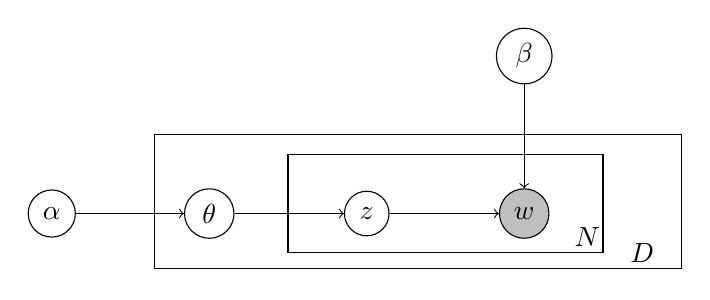
\begin{tikzpicture}

\node (theta) at (0,0) [circle, draw] {$\theta$};
\node (z) at (2,0) [circle, draw] {$z$};
\node[fill=lightgray] (w) at (4,0) [circle, draw] {$w$};
\node (alpha) at (-2,0) [circle, draw] {$\alpha$};
\node (b) at (4,2) [circle, draw] {$\beta$};
 
\draw[->] (alpha) -- (theta);
 
\draw[->] (theta.east) -- (z.west);
\draw[->] (z.east) -- (w.west);
\draw[->] (b.south) -- (w.north);
 
\draw (-.7,-.7) rectangle (6.,1);
\draw (1,-.5) rectangle (5,.75);
 
\node at (5.5,-.5) {$D$};
\node at (4.8,-.3) {$N$};
\end{tikzpicture} 
\caption{Bayesian plate notation for LDA}
\label{fig:plate-lda}
\end{figure}

\begin{figure}
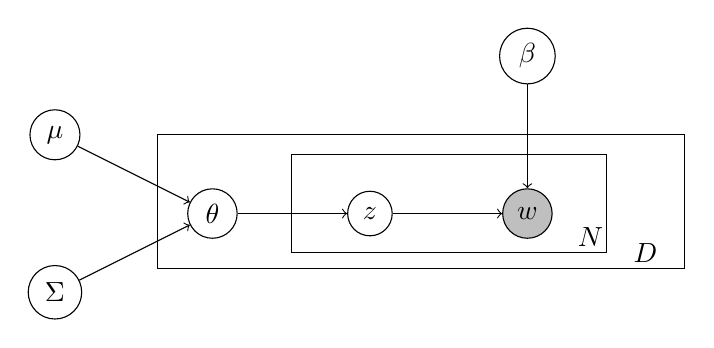
\begin{tikzpicture}
 
\node (theta) at (0,0) [circle, draw] {$\theta$};
\node (z) at (2,0) [circle, draw] {$z$};
\node[fill=lightgray] (w) at (4,0) [circle, draw] {$w$};
\node (b) at (4,2) [circle, draw] {$\beta$};

\node (mu) at (-2,1) [circle, draw] {$\mu$};
\node (sigma) at (-2,-1) [circle, draw] {$\Sigma$};
 
\draw[->] (mu) -- (theta);
\draw[->] (sigma) -- (theta);
 
\draw[->] (theta.east) -- (z.west);
\draw[->] (z.east) -- (w.west);
\draw[->] (b.south) -- (w.north);
 
\draw (-.7,-.7) rectangle (6.,1);
\draw (1,-.5) rectangle (5,.75);
 
\node at (5.5,-.5) {$D$};
\node at (4.8,-.3) {$N$};
\end{tikzpicture} 
\caption{Bayesian plate notation for CTM}
\label{fig:plate-ctm}
\end{figure}

Figure~\ref{fig:plate-lda} shows the so-called Bayesian plate notation for LDA that shows how the model assumes the text is generated:

\begin{itemize}[noitemsep]
\item For every document in the corpus (for a total of D documents):
\begin{itemize}[noitemsep]
\item From $\mathit{Dirichlet}(\alpha)$, draw $\theta_d$, the topic distribution for the document
\item For every word in the document (for a total of N words):
\begin{itemize}[noitemsep]
\item From $\mathit{Categorical}(\theta_d)$, draw $z_{d, n}$, the topic that the word belongs to
\item From $\mathit{Categorical}(\beta_{z_{d, n}})$ (the distribution of words for the topic $z_{d, n}$), draw $w_{d, n}$, the actual word
\end{itemize}
\end{itemize}
\end{itemize}

The Categorical distribution is simply a generalisation of the Bernoulli distribution with multiple outcomes. For example, given $\mathit{Categorical}([0.2, 0.5, 0.3])$, we will draw 0 with probability 0.2, 1 with probability 0.5 and 2 with probability 0.3.

The only variable that we can actually observe there is $w_{d, n}$, the vector of words in every document and hence it's shaded in grey on the diagram. The model parameters in this case are $\alpha$, the document-topic distribution, and $\beta$, the topic-word distribution.

It should be noted that these models show the exact assumed dependencies on the variables. For example, the vector $w_d$ is assumed to be independent of $\alpha$, since they're not directly connected by an arrow on the diagram. This means that expressing the conditional probability distributions is simpler, since unneeded variables can be dropped from the set we are conditioning on: $p(w_n | z_n, \theta, \beta, \alpha) = p(w_n | z_n, \beta)$.

The CTM (Figure~\ref{fig:plate-ctm}) has one difference from LDA: instead of assuming that the topics follow a Dirichlet distribution, it instead assumes that they follow $N(\mu, \Sigma)$, a Normal distribution. The generation process for $\theta_d$, the per-document topic distribution, is instead:

\begin{itemize}[noitemsep]
\item From $N(\mu, \Sigma)$, draw $\eta_d$
\item Normalize $\eta_d$: $\theta_d = f(\eta_d) $
\end{itemize}

and the normalisation function $f$ is defined as 

\begin{equation}
f(\eta_d) = \frac{e^{\eta_d}}{\sum\limits_i e^{\eta_{d, i}}}
\end{equation}

\chapter{Implementation}

\section{Training of the Correlated Topic Model}

\begin{table}
\begin{tabular}{| l | l |}
\hline
Variable & Description \\
\hline
$K$ & Number of topics in the corpus \\
$D$ & Number of documents in the corpus \\
$V$ & Number of words in the corpus (vocabulary size) \\
$N$ & Number of words in the document \\
$w_n$ & Nth word in the document \\
$c_n$ & Number of times the nth word occurs in the document \\
$\mu$ & Mean of the normal distribution of topics in the corpus \\
$\Sigma$ & Covariance matrix of the normal distribution of topics in the corpus \\
$\beta$ & $K \times V$ dimensional matrix of topic-word distributions \\
$\eta$ & Drawn unnormalised topic distribution for a certain document \\
$\theta$ & Normalised topic distribution for a certain document \\
$z$ & Drawn topic assignments for each word in the document \\
\hline
\end{tabular}
\caption{Definitions of the variables used in the Correlated Topic Model}
\label{tab:ctm-variables}
\end{table}

This section sets up the notation used throughout the whole dissertation and derives the training and the inference process for the Correlated Topic Model. The training process was mostly derived from Blei's original paper, however I provide some additions here so that the derivation is easier to understand. The derivation of the inference process is mine, however I used Blei's CTM implementation in C to verify my method.

Some variables in Table~\ref{tab:ctm-variables} are document-specific, for example, $\theta_d$ refers to the distribution of topics document $d$ is about. When this index is omitted, the document is assumed, for example, $w_n$ is the nth word in the document we are currently considering.

\subsection{Deriving the posterior distribution}

We aim to find the model parameters that maximise the likelihood bound on the whole corpus. In other words, what are the model parameters that we need to set so that the corpus we're inspecting is the most likely one?

First of all, given a document and the global model parameters, consider the distribution of the possible distributions of topics and the topic assignments:

\begin{equation}
p(\eta, z | w, \beta, \mu, \Sigma)
\end{equation}

Using Bayes' Theorem (and conditioning on the global model parameters $\beta, \mu, \Sigma$ throughout), this can be rewritten as 

\begin{equation}
\frac{p(\eta, z | \beta, \mu, \Sigma) p(w | \eta, z, \beta, \mu, \Sigma)}{p(w | \beta, \mu, \Sigma)}
\end{equation}

First, consider, $p(w | \eta, z, \beta, \mu, \Sigma)$, the probability of the document given all the model parameters and the topic assignments. Since all words in the document are independent of each other, this can be rewritten as a product:

\begin{align}
p(w | \eta, z, \beta, \mu, \Sigma) &= \prod\limits_{n=1}^N p(w_n | z_n, \eta, \beta, \mu, \Sigma) p(z_n | \eta, \beta, \mu, \Sigma)\\
& = \prod\limits_{n=1}^N p(w_n | z_n, \beta) p(z_n | \eta)
\end{align}

By inspecting the Bayesian plate notation of the model (Figure~\ref{fig:plate-ctm}), it can be seen that $w_n$ is only dependent on the topic assigment $z_n$ and the per-topic word distribution $\beta$, hence all of the other variables we are conditioning on can be removed from consideration. Similarly with $z_n$: it's only dependent on $\eta$.

The denominator is the probability of the document given the global model parameters and it has to be calculated by marginalising over all possible distributions of topics and topic assignments:

\begin{align}
p(w | \beta, \mu, \Sigma) & = \int p(w | \eta, \beta) p(\eta | \mu, \Sigma) d\eta \\
& =\int p(\eta | \mu, \Sigma)  \prod\limits_{n=1}^N p(w_n | \eta, \beta) d\eta \\
& =\int p(\eta | \mu, \Sigma)  \prod\limits_{n=1}^N \sum\limits_{z_n=1}^K p(z_n | \eta) p(w_n | z_n, \beta) d\eta
\end{align}

In this expansion, we first integrate over all possible distributions of topics $\eta$, then the integrand is expanded to be a product over all words in the document and then, finally, we integrate over all possible topic assignments (since the integral is discrete, it turns into a sum). As in the previous derivation, due to the independence assumptions, we liberally add and remove the variables we are conditioning on to simplify the expression.

The final expression, as it appears in Blei's paper, is

\begin{equation}
\frac{p(\eta | \mu, \Sigma) \prod\limits_{n=1}^N p(w_n | z_n, \beta) p(z_n | \eta)}{\int p(\eta | \mu, \Sigma)  \prod\limits_{n=1}^N \sum\limits_{z_n=1}^K p(z_n | \eta) p(w_n | z_n, \beta) d\eta}
\end{equation}

There are two problems with this expression's denominator (the marginal probability of the document). First, it contains a summation over $K$ possible values of the topic of the nth word in the document, $z_n$, which is inside a product over the $N$ words in the document, thus the integrand will contain $K^N$ terms: intractable with the sizes of the data used in this project. Worse even, the distributions $p(z_n | \eta)$ and $p(\eta | \mu, \Sigma)$ are not conjugate to each other, hence the integral over $\eta$ cannot be computed analytically.

\subsection{Using variational methods to approximate the likelihood bound}

To solve this problem, Blei uses variational methods, which involve approximating the posterior distribution with a simpler one, called the variational distribution. The parameters of the distribution are fit to the true posterior (by minimizing the Kullback-Leibner divergence) and the variational distribution is used as a substitute for the posterior.

The definition of the distribution is

\begin{equation}
q(\eta, z | \lambda, \nu, \phi) = \prod\limits_{i=1}^K q(\eta_i|\lambda_i, \nu_i^2) \prod\limits_{n=1}^N q(z_n | \phi_n)
\end{equation}

Here, the variational distribution of the per-document topic distribution $\eta$ is $K$ independent normal variables with means $\lambda$ and standard deviations $\nu$.

Minimizing the Kullback-Leibner divergence between the variational distribution and the true posterior is the same as optimizing the parameters of the variational distribution so that it maximizes the probability of the document. This is equivalent to maximizing the log probability of the document, which can be bounded as

\begin{align}\label{eq:likelihood-bound}
\log p(w | \beta, \mu, \Sigma) & \geq \mathbb{E}_q[\log p(\eta|\mu, \Sigma)] \\
& + \sum\limits_{n=1}^N \mathbb{E}_q[\log p(z_n | \eta)] \\
& + \sum\limits_{n=1}^N \mathbb{E}_q[\log p(w_n | z_n, \beta)] \\
& + \mathbb{H}(q)
\end{align}

Here, the expectation is taken with respect to the relevant variational distributions $q$ and $\mathbb{H}(q)$ is the entropy of the variational distribution.

The components of the likelihood bound are then rewritten in terms of the variational parameters $\lambda, \nu, \phi$:

\begin{align}
\mathbb{E}_q[\log p(\eta|\mu, \Sigma)] & = \frac{1}{2} \log |\Sigma^{-1}| - \frac{K}{2} \log 2 \pi - \frac{1}{2}\mathbb{E}_q[(\eta - \mu)^T\Sigma^{-1}(\eta - \mu)] \\ \label{eq:eta_mu_sigma}
& = \frac{1}{2} \log |\Sigma^{-1}| - \frac{K}{2} \log 2 \pi - \frac{1}{2}(\mathit{Tr}(\mathit{diag}(\nu^2)\Sigma^{-1}) + (\lambda - \mu)^T\Sigma^{-1}(\lambda - \mu))
\end{align}

\begin{align}
\mathbb{E}_q[\log p(z_n | \eta)] & = \mathbb{E}_q[\eta^Tz_n] - \mathbb{E}_q[\log \sum\limits_{i=1}^K e^{\eta_i}] \\
& \geq \mathbb{E}_q[\eta^Tz_n] - \zeta^{-1}(\sum\limits_{i=1}^K\mathbb{E}_q[e^{\eta_i}] + 1 - \log\zeta \\
& = \sum\limits_{i=1}^K\lambda_i\phi_{n, i} - \zeta^{-1}(\sum\limits_{i=1}^Ke^{\lambda_i + \nu_i^2 / 2}) + 1 - \log\zeta
\end{align}

Here, the term $\mathbb{E}_q[\log \sum\limits_{i=1}^K e^{\eta_i}]$ was bound by a Taylor expansion, introducing an extra parameter $\zeta$.

\begin{equation}
\mathbb{E}_q[\log p(w_n | z_n, \beta)] = \sum\limits_{i=1}^K\phi_{n,i}\log\beta_{i, w_n}
\end{equation}

\begin{equation}
\mathbb{H}(q) = \sum\limits_{i=1}^K\frac{1}{2}(\log\nu_i^2 + \log 2 \pi + 1) - \sum\limits_{n=1}^N\sum\limits_{i=1}^K\phi_{n,i}\log\phi_{n,i}
\end{equation}

\subsection{Maximising the likelihood bound}

Finally, the optimisation of the likelihood bound happens by iteratively maximising it with respect to each one of the variational parameters.

First, the maximisation of the bound with respect to $\zeta$ can be performed analytically:

\begin{equation}
\hat\zeta = \sum\limits_{i=1}^Ke^{\lambda_i + \nu_i^2 / 2}
\end{equation}

$\phi$ has a maximum at

\begin{equation}
\hat\phi_{n, i} \propto e^{\lambda_i}\beta_{i, w_n} \label{eq:phiopt}
\end{equation}

($\phi$ then has to be normalised).

For maximisation with respect to $\lambda$ and $\nu^2$, numerical methods are used with derivatives

\begin{align}
dL/d\lambda & = -\Sigma^{-1}(\lambda - \mu) + \sum\limits_{n=1}^N\phi_{n, 1:K} - (N/\zeta)e^{\lambda + \nu^2/2} \\
dL/d\nu^2 & = -\mathit{diag}(\Sigma^{-1})/2 - \frac{N}{2\zeta}e^{\lambda + \nu^2/2} + \frac{1}{2\nu^2}
\end{align}

Blei's paper suggests using the conjugate gradient algorithm to optimise $\lambda$ and Newton's method for each coordinate of $\nu^2$, however, I found that I got better performance (both in convergence rates and the speed of the model) when using the limited-memory Broyden-Fletcher-Goldfarb-Shanno algorithm with box constraints (L-BFGS-B) to optimise for the whole vector $\nu^2$. I didn't write my own implementations of the conjugate gradient or the L-BFGS-B algorithm: they were available as a part of SciPy.

Once these variational parameters have been found, they are used to estimate the global model parameters:

\begin{align}
\hat\beta_i & \propto \sum\limits_d\phi_{d, i}N_d \\ \label{eq:betaopt}
\hat\mu & = \frac{1}{D} \sum\limits_d\lambda_d \\ 
\hat\Sigma & = \frac{1}{D} \sum\limits_d I\nu^2_d + (\lambda_d - \hat\mu)(\lambda_d - \hat\mu)^T
\end{align}

\subsection{Final algorithm of the training process}

To convert these equations to an algorithm, we need to address some performance considerations. The likelihood bound (\ref{eq:likelihood-bound}) has several sums over all words n in the document, which is wasteful, since each term in the sum will be the same for the same word. Hence, we split the document into $w_n$, a vector of distinct words, and $c_n$, a vector of counts of these words. $n$ now will refer to the nth distinct word in the document. The matrix $\phi_{n, i}$ now refers to the nth distinct word in the document and ith topic. Finally, the terms inside the sums only have to be calculated once (for each distinct word) and weighted by the number of times that word appears in the document.

The overall training process is as follows: set some initial model parameters and use those to perform variational inference on every document. Use the variational parameters to update the model parameters and repeat until the likelihood bound converges (fractional change is less than a certain threshold).

These steps are described in algorithms~\ref{alg:variational_inference} and~\ref{alg:expectation_maximisation}. 

In the original paper, this algorithm is called Variational EM (Expectation-Maximisation). The classic EM algorithm consists of two steps: the E step, where some sort of a function of the model parameters is calculated or expressed, and the M step, where that function is maximised. Here, the E step is the variational inference process (where we express the likelihood bound on the document as a function of the parameters of the variational distribution (fit to each document) and the global model parameters) and the M step is where the variational parameters for every document are combined to update the global model parameters.

\documentclass{article}
\usepackage[noend]{algpseudocode}
\usepackage[]{algorithm}
\usepackage{amsmath}
\usepackage[cm]{fullpage}
\newcommand{\var}[1]{{\operatorname{\mathit{#1}}}}

\begin{document}
\begin{algorithm}
   \caption{Variational Inference for a document}
   \label{alg:variational_inference}
   \Comment{$\var{mod-params}$ is a tuple $(\mu, \Sigma, \beta), \var{var-params}$ is a tuple $(\zeta, \phi, \lambda, \nu^2)$.}
   \begin{algorithmic}[1]
      \Function{optimize-zeta}{$\lambda, \nu^2$}
      \State \Return $\sum{}{e^{\lambda + \frac{1}{2}\nu^2}}$
      \EndFunction 
      \Function{optimize-lambda}{$\var{var-params}, \var{mod-params}, w, n$}
      \State The objective functions use the $\lambda$ given in the function parameters instead of the one in $\var{var-params}$.
    	  \Function{objective-lambda}{$\lambda, \var{var-params}, \var{mod-params}, w, n$}
		      \State\Return $\frac{1}{2}(\lambda - \mu)^T\Sigma^{-1}(\lambda-\mu) - \sum{}{\phi} + \frac{N}{\zeta}\sum{}{e^{\lambda + \frac{1}{2}\nu^2}}$
	      \EndFunction
     	  \Function{objective-lambda-gradient}{$\lambda, \var{var-params}, \var{mod-params}, w, n$}
		      \State\Return $\Sigma^{-1}(\lambda - \mu) - \sum{}{\phi} + \frac{N}{\zeta}\sum{}{e^{\lambda + \frac{1}{2}\nu^2}}$
	      \EndFunction
	  \State $\lambda\gets $ result from a SciPy minimizer using functions \Call{objective-lambda}{} and \Call{objective-lambda-gradient}{}
      \State \Return $\lambda$
      \EndFunction
      \Function{optimize-nu-sq}{$\lambda, \nu^2$}
      
	\State The objective functions use the $\nu^2$ given in the function parameters instead of the one in $\var{var-params}$
    	  \Function{objective-nu-sq}{$\nu^2, \var{var-params}, \var{mod-params}$}
		      \State\Return $trace(\frac{1}{2}diag(\nu^2)\Sigma^{-1}) + \frac{N}{\zeta}\sum{}{e^{\lambda + \frac{1}{2}\nu^2}} - \frac{1}{2}\sum{}{(1 + ln(2\pi \nu^2))}$
	      \EndFunction
     	  \Function{objective-nu-sq-gradient}{$\nu^2, \var{var-params}, \var{mod-params}$}
		      \State\Return $\frac{1}{2}diag(\Sigma^{-1}) + \frac{N}{2\zeta}e^{\lambda + \frac{1}{2}\nu^2} - \frac{1}{2\nu^2}$
	      \EndFunction
	  \State $\nu^2\gets $ result from a SciPy minimizer using functions \Call{objective-nu-sq}{} and \Call{objective-nu-sq-gradient}{}
      \State \Return $\nu^2$
      \EndFunction
      \Function{optimize-phi}{$\var{var-params}, \var{mod-params}, w, n$}
		\State $\phi_{n,i}\gets e^{\lambda_i}\beta_{i, w_n}n_n$
	  \State Normalize $\phi$ so that every row sums up to 1
      \State \Return $\phi$
      \EndFunction
   
      \Function{variational-inference}{$\var{mod-params}, w, n$}
      \State Initialize the variational parameters: $\var{var-params}=(\zeta=10, \phi=1, \lambda=0, \nu^2=1$)
      \While{change in likelihood bound $>$ threshold}
      \State $\zeta\gets \Call{optimize-zeta}{\lambda, \nu^2}$
      \State $\lambda\gets \Call{optimize-lambda}{\var{var-params}, \var{mod-params}, w, n}$
      \State $\zeta\gets \Call{optimize-zeta}{\lambda, \nu^2}$
      \State $\nu^2\gets \Call{optimize-nu-sq}{\var{var-params}, \var{mod-params}}$
      \State $\zeta\gets \Call{optimize-zeta}{\lambda, \nu^2}$      
      \State $\phi\gets \Call{optimize-phi}{\var{var-params}, \var{mod-params}, w, n}$
      \EndWhile
    \State \Return $\var{var-params}$
    \EndFunction
\end{algorithmic}
\end{algorithm}

\begin{algorithm}
	\caption{Model parameter inference for the whole corpus}
	\label{alg:expectation_maximisation}
	\begin{algorithmic}[1]
		\Function{inference}{$\var{corpus}, K$}
			\State Initialize the model parameters: $\var{mod-params}=(\mu = 0, \Sigma=I, \beta=\var{priors})$
			\While{change in likelihood bound $>$ threshold}
				\State $\var{var-params}\gets \Call{variational-inference}{\var{mod-params}, w, n}$ for all $(w, n)$ in $\var{corpus}$
				
				\State $\mu \gets \frac{1}{D}\sum\limits_{v \in \var{var-params}}{v.\lambda}$
				\State $\Sigma \gets \frac{1}{D}\sum\limits_{v \in \var{var-params}}{(diag(v.\nu^2) + (v.\lambda - \mu)(v.\lambda - \mu)^T)}$
				\State $\beta \gets 0$
				\For{$d$ in $1..D$}
					\For{$w$ in $1..len(corpus_d.w)$}
						\For {$i$ in $1..K$}
							$\beta_{i, w} \gets \beta_{i, w} + corpus_d.n_w \times \var{mod-params}_d.\phi_{w, i}$
						\EndFor
					\EndFor
				\EndFor
				\State Normalize $\beta$ so that every row sums up to 1
			\EndWhile
			\State\Return $\var{mod-params}$
		\EndFunction
	\end{algorithmic}
\end{algorithm}

\end{document}

\section{Incorporating priors into the Model}

In the training process, from \eqref{eq:phiopt} and \eqref{eq:betaopt} it follows that a zero entry in the $\beta$ matrix that the training process is initialized with will carry through to the $\phi$ matrices for every document and will be fed back into the updated $\beta$. Since the parameters are optimised using gradient ascent, this essentially enforces a constraint on $\beta$ so that it has zeros in set places.

This has the effect of setting pathway-gene membership priors and ensures that the inferred topic structure is referring to the actual pathways, so the results of the inference process will allow us to make judgements about real-world phenomena.

\section{Classification process}

Using the variational parameters inferred for every document and the global model parameters, it is possible to find the expected value of $\theta$, the document-topic distribution. Since $\theta = f(\eta)$, a normalised vector, finding the expected value of $\eta$ is sufficient. However, this involves performing an integration over the space of all possible $\eta$, which is intractable. Hence, this integral has to be approximated using Monte Carlo and importance sampling (TODO: reference an importance sampling paper):

\begin{align}
\hat\theta \propto \frac{1}{N}\sum\limits_{s=1}^N f(\eta_s) \frac{p(\eta_s | w, \mu, \Sigma, \beta)}{q(\eta_s | \lambda, \nu)}
\end{align}

$\eta$ is sampled $N$ times from the distribution described by a probability density function $q$. The easiest way to sample $\eta$ is from the variational distribution that was fitted to the document: recall that $\eta \sim N(\lambda, \mathit{diag}(\nu))$ and so $q(\eta_s | \lambda, \nu) = \mathit{NormalPDF}(\eta_s, \lambda, \nu)$.

$p$ is the density function of the actual distribution whose expected value we are looking for: in essence, we're trying to estimate $\mathbb{E}(\theta | w, \mu, \Sigma, \beta)$. According to the Bayes' theorem, we can invert the conditioning:

\begin{align}
p(\eta_s | w, \mu, \Sigma, \beta) &= \frac{p(w | \eta_s, \mu, \Sigma, \beta)p(\eta_s | \mu, \Sigma, \beta)}{p(w | \mu, \Sigma, \beta)}\\
&= p(w | \eta_s, \beta) p(\eta_s | \mu, \Sigma)
\end{align}

Unnecessary conditioning can also be dropped ($w$ only depends on $\eta_s$ and $\beta$ and $\eta_s$ only depends on $\mu$ and $\Sigma$). In addition, the marginal probability $p(w | \mu, \Sigma, \beta)$ is dropped: it doesn't depend on the sampled value of $\eta_s$ and so will just be a scalar multiplier on the final estimated value of $\hat\eta$, which will be have to be normalised to get $\hat\theta$ anyway, thus the multiplier will be discarded.

It will be easier to express and calculate the logarithm of this value: in that case, the weight assigned to every sample $f(\eta_s)$ will be

\begin{align}
&\log \frac{p(w | \eta_s, \mu, \Sigma, \beta)p(\eta_s | \mu, \Sigma, \beta)}{p(w | \mu, \Sigma, \beta)} = \\
&\log p(w | \eta_s, \beta) + \log p(\eta_s | \mu, \Sigma) - \log q(\eta_s | \lambda, \nu)
\end{align}

The remaining terms of this weight are derived as follows:

\begin{align}
\log p(w | \eta_s, \beta) = \log p(w | \theta_s, \beta) &= \log \prod\limits_{n=1}^N p(w_n | \theta, \beta)^{c_n}\\
&= \log \prod\limits_{n=1}^N \left(\sum\limits_{i=1}^K \theta_i \beta_{i, w_n}\right)^{c_n}\\
&= \sum\limits_{n=1}^N c_n \log \sum\limits_{i=1}^K \theta_i \beta_{i, w_n}
\end{align}

The probability of a specific document given its topic distribution $\theta_s$ and the topic-word distribution $\beta$ is easy to express, since all words in the document are independent and we know exactly what is the probability of drawing a specific topic and drawing a specific word from a specific topic. Furthermore, taking the logarithm only leaves sums in the final expression: this will later allow to convert it to a series of vector and matrix products, which helps the speed of the actual implementation.

The remaining term can be simply copied over from Equation~\ref{eq:eta_mu_sigma}:

\begin{align}
\log p(\eta_s | \mu, \Sigma) = \frac{1}{2} \log |\Sigma^{-1}| - \frac{K}{2} \log 2 \pi - \frac{1}{2}(\eta - \mu)^T\Sigma^{-1}(\eta - \mu)
\end{align}

TODO python code or pseudocode

\section{Implementation in code and code optimisation}

To implement the training process for the model, I used Python, perhaps an unusual choice given the large amount of numerical computation that needs to be done and the poor performance of Python on these kinds of tasks. However, Python allows for extremely dense and expressive code, as well as has a REPL (Read-Eval-Print Loop), which allows for quick prototyping, implementation and debugging. The unsuitability of Python for numerical calculations is fixed by \texttt{NumPy}\cite{DBLP:journals/corr/abs-1102-1523}, a linear algebra library, that allows fast matrix operations in native code (using either routines provided by \texttt{NumPy} or more advanced numerical libraries that support the Basic Linear Algebra Subsystem (BLAS) API, such as ATLAS or OpenBLAS). In addition, \texttt{NumPy} integrates well with \texttt{SciPy}, a scientific computing library that provides useful routines, for example, for working with probability distributions or numerical optimisation.

Despite using \texttt{NumPy}, I still had performance issues which would have made working with the real-world datasets very inconvenient. I used \texttt{cProfile}, a Python profiler, to investigate those.

\begin{figure}
\begin{Verbatim}[fontsize=\scriptsize]
   ncalls  tottime  percall  cumtime  percall filename:lineno(function)
     5596   56.686    0.010   60.062    0.011 variational_inference.py:34(f_lambda)
      616   22.737    0.037   57.636    0.094 variational_inference.py:70(likelihood_bound)
  5599536    9.381    0.000   33.919    0.000 math_utils.py:10(safe_log)
  5587240    7.286    0.000    7.286    0.000 {method 'clip' of 'numpy.generic' objects}
  5639219    6.708    0.000    6.708    0.000 {method 'reduce' of 'numpy.ufunc' objects}
       48    5.111    0.106  118.752    2.474 variational_inference.py:96(variational_inference)
    40346    4.260    0.000    4.260    0.000 {sum}
  5587240    4.154    0.000   11.132    0.000 {method 'max' of 'numpy.generic' objects}
  5602512    3.854    0.000   15.054    0.000 [...]\numpy\core\fromnumeric.py:2050(amax)
  5599536    2.196    0.000    9.512    0.000 [...]\numpy\core\fromnumeric.py:1566(clip)
     5243    2.006    0.000    2.970    0.001 variational_inference.py:25(f_dlambda)
  5602512    1.329    0.000    7.045    0.000 [...]\numpy\core\_methods.py:25(_amax)
        2    1.127    0.564    1.620    0.810 [...]\numpy\lib\npyio.py:631(loadtxt)
        1    0.542    0.542  128.322  128.322 expectation_maximization.py:31(expectation_maximization)
    15759    0.362    0.000    0.362    0.000 {zip}
    11016    0.221    0.000    0.849    0.000 variational_inference.py:49(f_nu_sq)
    29299    0.188    0.000    0.188    0.000 {method 'dot' of 'numpy.ndarray' objects}
    26757    0.176    0.000    0.176    0.000 {numpy.core.multiarray.array}
      472    0.140    0.000   63.618    0.135 [...]\scipy\optimize\optimize.py:792(_minimize_bfgs)
     6129    0.135    0.000    0.135    0.000 {method 'split' of 'str' objects}
    36235    0.132    0.000    1.185    0.000 [...]\numpy\core\fromnumeric.py:1623(sum)
    11016    0.123    0.000    0.365    0.000 variational_inference.py:64(f_dnu_sq)
     2531    0.122    0.000   53.814    0.021 [...]\scipy\optimize\linesearch.py:101(scalar_search_wolfe1)
  1692604    0.118    0.000    0.118    0.000 {len}
    16354    0.089    0.000    0.089    0.000 {numpy.core._dotblas.dot}
      472    0.085    0.000    1.356    0.003 [...]\scipy\optimize\lbfgsb.py:198(_minimize_lbfgsb)
    11632    0.061    0.000    0.061    0.000 {method 'trace' of 'numpy.ndarray' objects}
    11680    0.060    0.000    0.099    0.000 [...]\numpy\lib\twodim_base.py:242(diag)
      616    0.048    0.000    0.066    0.000 [...]\numpy\linalg\linalg.py:1679(det)
    21855    0.047    0.000   63.928    0.003 [...]\scipy\optimize\optimize.py:279(function_wrapper)
        1    0.046    0.046  130.036  130.036 D:/Projects/part2-dissertation/ctm-test.py:6(<module>)
    39010    0.042    0.000    0.042    0.000 {isinstance}
     4744    0.040    0.000    2.754    0.001 [...]\scipy\optimize\linesearch.py:84(derphi)
        1    0.039    0.039    0.039    0.039 {method 'round' of 'numpy.ndarray' objects}
6120/3060    0.038    0.000    0.039    0.000 [...]\numpy\lib\npyio.py:775(pack_items)
    22465    0.038    0.000    0.038    0.000 {numpy.core.multiarray.zeros}
     4744    0.027    0.000   50.928    0.011 [...]\scipy\optimize\linesearch.py:80(phi)
    12296    0.025    0.000    0.025    0.000 {method 'clip' of 'numpy.ndarray' objects}
    36235    0.024    0.000    1.014    0.000 [...]\numpy\core\_methods.py:31(_sum)
        1    0.023    0.023    0.024    0.024 [...]\spyderlib\widgets\externalshell\sitecustomize.py:501(run)
\end{Verbatim}
\caption{\texttt{cProfile} output for the CTM training before the optimisation on 12 drugs, 23 pathways, 284 genes}
\label{fig:ctm-profile-before}
\end{figure}

Figure~\ref{fig:ctm-profile-before} shows the \texttt{cProfile} output for my implementation of CTM training process before optimisation, sorted by \texttt{totttime}. \texttt{tottime} represents total time spent in just the given function and not in any functions that it calls, whereas \texttt{cumtime} represents the total time spent in the function, from entry to exit.

The training was run on 1/100th of all drugs, 1/10th of all pathways and 1/10th of all genes, resulting in a thinned dataset of 12 drugs, 23 pathways and 284 genes. It took about 2 minutes (\texttt{cumtime} for the EM function \texttt{expectation\_maximization} is 128 seconds), which implies that the training time for the whole dataset would have been more than 20000 minutes (since the process involves matrix multiplications, it is supra-linear in most of the input sizes), which is unacceptable.

It is immediately obvious that the program spends most of its time recalculating the likelihood bound (\texttt{likelihood\_bound}) and the objective function for the optimisation of the bound with respect to $\lambda$ (\texttt{f\_lambda}). These two functions in total account for almost all the time (117 seconds) the program runs.

\begin{figure}
\begin{Verbatim}[fontsize=\scriptsize]
def likelihood_bound(v_params, m_params, doc, counts):
    N = sum(counts)
    
    #E_q(logp(eta|mu,sigma))
    result = 0.5 * safe_log(np.linalg.det(m_params.inv_sigma))
    result -= 0.5 * safe_log(2 * np.pi) * len(m_params.beta)
    result -= 0.5 * (np.diag(v_params.nu_sq).dot(m_params.inv_sigma)).trace()
    lambda_mu = v_params.lambd - m_params.mu
    result -= 0.5 * lambda_mu.dot(m_params.inv_sigma.dot(lambda_mu))
    
    #E_q(logp(z|eta))
    result += sum([c * v_params.lambd[i] * v_params.phi[n, i]\
        for (n, c) in zip(xrange(len(doc)), counts) for i in xrange(len(m_params.beta))])
    result -= N * (1.0 / v_params.zeta * np.sum(np.exp(v_params.lambd + 0.5 * v_params.nu_sq))\
        - 1 + safe_log(v_params.zeta))
    
    #E_q(logp(w|mu,z,beta))
    result += sum([c * v_params.phi[n, i] * safe_log(m_params.beta[i, doc[n]])\
        for (n, c) in zip(xrange(len(doc)), counts) for i in xrange(len(m_params.beta))])
    
    #H(q)
    result += np.sum(0.5 * (1 + safe_log(v_params.nu_sq * 2 * np.pi)))
    result -= np.sum([c * v_params.phi[n, i] * safe_log(v_params.phi[n, i])\
        for (n, c) in zip(xrange(len(doc)), counts) for i in xrange(len(m_params.beta))])
    
    return result
\end{Verbatim}
\caption{Code of the likelihood bound calculation before optimisation}
\label{fig:code-before-optimisation}
\end{figure}

Since \texttt{f\_lambda} is just the negated likelihood bound calculation with only the terms that depend on $\lambda$, the bulk of the performance improvements will come from optimising \texttt{likelihood\_bound} (Figure~\ref{fig:code-before-optimisation}).

The biggest issue here is the use of various Pythonisms like list comprehensions and the \texttt{zip} function. While the first term does use the \texttt{dot} function (for \texttt{NumPy} matrix multiplication), the calculation of the last 3 terms of the likelihood bound doesn't. It involves performing very similar operations: iterating over all distinct words in the document and all topics (thus creating a tuple \texttt{(n, c, i)} for the word index, word number and the topic index), multiplying \texttt{c * v\_params.phi[n, i]} by a different term (for every term out of these three terms in the likelihood bound), then creating an ad-hoc list of these subterms and then finally summing all items in this list to get to the actual term.

Even if this redundancy were eliminated, this code is still evaluated by the Python interpreter, which is still extremely wasteful. Hence I tried to convert the code to use matrix operations, as these would be evaluated in native code.

First of all, the \texttt{c * v\_params.phi[n, i]} term is converted to a vector \texttt{weighted\_sum\_phi} that is updated only when \texttt{phi} changes (during the variational inference loop): \texttt{weighted\_sum\_phi = doc\_counts.dot(phi)}. This vector represents the term $\sum\limits_n\ c_n\phi_{n, i}$. Now the first term can be simply rewritten as \texttt{v\_params.weighted\_sum\_phi.dot(v\_params.lambd)}.

In the \texttt{safe\_log(m\_params.beta[i, doc[n]]} term, it seems as if we do need to perform an explicit iteration over the matrix, as we need to find $\beta_{i, w_n}$. Luckily, \texttt{NumPy} supports indexing a matrix not only with a scalar, but also with a vector. In this case, \texttt{m\_params.beta.T[doc]} will transpose the matrix (notice that in the original expression, \texttt{phi} is indexed by \texttt{[n, i]}, whereas \texttt{beta} has the indices swapped) and return another matrix of the same shape as \texttt{phi}. The final expression is \texttt{np.sum(np.dot(counts, np.multiply(v\_params.phi, safe\_log(m\_params.beta.T[doc]))))}, where \texttt{np.multiply} is the Hadamard product of two matrices.

Similarly, the final term is converted to \texttt{np.sum(np.dot(counts, np.multiply(v\_params.phi, safe\_log(v\_params.phi))))}.

Another bottleneck in the above profile is the \texttt{safe\_log} function. I had to write and use it because the training process requires taking a logarithm of $\beta$: recall that certain positions in $\beta$ are enforced to always be zero, which causes the normal logarithm function to return -infinity. My workaround for this was to clamp the output of the logarithm function to always return at least $-10^5$. However, this essentially meant having to traverse every matrix once again, which added up to massive performance losses since \texttt{safe\_log} had to be called so much. I hence decided to instead set the required entries of $\beta$ to $10^{-100}$ every EM cycle (of which there would be less than 100), which meant that the builtin logarithm function wouldn't break anymore.

Even after rewriting the likelihood bound calculation, it still was a major bottleneck: it had to be performed every variational inference cycle for every document, since the termination criterion is based on the magnitude of changes in the bound. One solution to this would be not calculating the likelihood bound every iteration, but this resulted in worse performance: another variational inference cycle (2500ms in the unoptimised program) was more expensive than checking the bound (94ms). To speed this up, I used \texttt{numexpr}, a package that compiles operations on \texttt{NumPy} arrays into its own internal virtual machine bytecode and supports multithreaded computations on arrays. This involved rewriting some code for the likelihood bound calculation (since \texttt{numexpr} only supports some operators and mathematical functions) and passing it as a string to the evaluator. Interestingly enough, I did not get an improvement when making the objective functions for the $\nu^2$ and $\lambda$ optimisation use \texttt{numexpr}.

In addition, the variational inference process requires calling the \texttt{SciPy} function minimizer for $\lambda$ and $\nu^2$ every training iteration, which requires an initial value to start its search from. Recycling the variational parameters to continue the search from the previous iteration gave yet another performance improvement.

I also recompiled my \texttt{NumPy} distribution to use the Intel Math Kernel Library as its backend. Free for academic and personal use, Intel MKL provides a linear algebra library that implements the BLAS (Basic Linear Algebra Subsystem) API, optimized for manycore Intel CPUs. This benefits not only \texttt{NumPy}'s matrix multiplication, but also \texttt{numexpr}'s VM that can use the Intel Vector Math Library (VML) for faster operations on vectors.

Since the variational inference process is independent for every document, it can be parallelized across multiple cores. However, because of the Python Global Interpreter Lock, only one thread can execute Python bytecode at a time. This meant that I had to launch several Python processes if I wanted to take advantage of my CPU's capabilities. While this did provide an increase in CPU usage, it resulted in worse performance than using \texttt{numexpr} and Intel MKL's natural multithreading capabilities.

\begin{figure}
\begin{Verbatim}[fontsize=\scriptsize]
   ncalls  tottime  percall  cumtime  percall filename:lineno(function)
    88460    5.939    0.000    7.237    0.000 [...]\numexpr\necompiler.py:662(evaluate)
   639494    1.683    0.000    1.683    0.000 {method 'dot' of 'numpy.ndarray' objects}
    99000    1.664    0.000    3.280    0.000 [...]\scipy\optimize\linesearch.py:397(_cubicmin)
   151068    1.475    0.000    3.099    0.000 variational_inference.py:42(f_lambda)
   413096    1.426    0.000    1.426    0.000 {method 'reduce' of 'numpy.ufunc' objects}
     2340    1.344    0.001   27.691    0.012 variational_inference.py:105(variational_inference)
    69397    1.287    0.000    3.232    0.000 variational_inference.py:57(f_nu_sq)
        2    1.122    0.561    1.587    0.793 [...]\numpy\lib\npyio.py:631(loadtxt)
    17692    1.121    0.000   10.651    0.001 variational_inference.py:75(likelihood_bound)
    10672    1.062    0.000    5.928    0.001 [...]\scipy\optimize\lbfgsb.py:198(_minimize_lbfgsb)
    69397    0.847    0.000    1.040    0.000 variational_inference.py:70(f_dnu_sq)
   521216    0.771    0.000    0.771    0.000 {numpy.core.multiarray.array}
   412986    0.636    0.000    1.358    0.000 [...]\numpy\core\numeric.py:2428(seterr)
    17692    0.635    0.000    0.952    0.000 [...]\numpy\linalg\linalg.py:1599(slogdet)
   218760    0.632    0.000    0.632    0.000 {numpy.core._dotblas.dot}
   107493    0.621    0.000    1.557    0.000 [...]\scipy\optimize\linesearch.py:431(_quadmin)
    88460    0.570    0.000    0.646    0.000 [...]\numexpr\necompiler.py:462(getContext)
   370334    0.543    0.000    2.203    0.000 [...]\numpy\core\fromnumeric.py:1623(sum)
     9900    0.475    0.000    8.050    0.001 [...]\scipy\optimize\linesearch.py:452(_zoom)
   412986    0.460    0.000    0.496    0.000 [...]\numpy\core\numeric.py:2524(geterr)
    87089    0.455    0.000    0.455    0.000 {method 'trace' of 'numpy.ndarray' objects}
    89429    0.442    0.000    0.748    0.000 [...]\numpy\lib\twodim_base.py:242(diag)
    33113    0.437    0.000    0.522    0.000 variational_inference.py:33(f_dlambda)
   118800    0.409    0.000    2.965    0.000 [...]\scipy\optimize\linesearch.py:237(phi)
   252950    0.388    0.000    0.388    0.000 {numpy.core.multiarray.zeros}
   253578    0.291    0.000    7.143    0.000 [...]\scipy\optimize\optimize.py:279(function_wrapper)
    10672    0.285    0.000   10.910    0.001 [...]\scipy\optimize\optimize.py:1101(_minimize_cg)
   478523    0.282    0.000    0.829    0.000 [...]\numpy\core\numeric.py:394(asarray)
    21344    0.264    0.000   17.353    0.001 [...]\scipy\optimize\_minimize.py:37(minimize)
   490325    0.252    0.000    0.252    0.000 {isinstance}
    20645    0.240    0.000    1.215    0.000 [...]\scipy\optimize\linesearch.py:101(scalar_search_wolfe1)
     4743    0.208    0.000    0.208    0.000 {sum}
    91601    0.206    0.000    0.206    0.000 {zip}
   412986    0.170    0.000    0.170    0.000 {numpy.core.umath.seterrobj}
   206493    0.170    0.000    0.198    0.000 [...]\numpy\core\numeric.py:2809(__init__)
   206493    0.167    0.000    0.892    0.000 [...]\numpy\core\numeric.py:2813(__enter__)
   206493    0.160    0.000    0.793    0.000 [...]\numpy\core\numeric.py:2818(__exit__)
   370334    0.157    0.000    1.442    0.000 [...]\numpy\core\_methods.py:31(_sum)
   176920    0.141    0.000    0.141    0.000 [...]\numexpr\necompiler.py:611(getType)
     6129    0.134    0.000    0.134    0.000 {method 'split' of 'str' objects}
\end{Verbatim}
\caption{\texttt{cProfile} output for the CTM training after the optimisation on 117 drugs, 23 pathways, 284 genes}
\label{fig:ctm-profile-after}
\end{figure}

Finally, Figure~\ref{fig:ctm-profile-after} shows the profiling data of the resultant program, with training run on 1/10th of all drugs, 1/10th of all pathways and 1/10th of all genes (in essence, 10 times as many drugs as the previous thinned dataset). The training time was 30 seconds, which is a massive 40x performance improvement on the unoptimised program (indeed, the training time for the whole real-world dataset was about 8-9 hours). The bulk of the time is now spent in \texttt{numexpr}'s evaluator and a single likelihood bound calculation now takes 1ms on average (as opposed to the previous program's 94ms). More calls are now made to \texttt{numpy.core.\_dotblas.dot}, which is the native \texttt{NumPy} matrix multiplication routine.

Interestingly, these changes made the code shorter and perhaps more readable (Figure~\ref{fig:code-after-optimisation}).

\begin{figure}
\begin{Verbatim}[fontsize=\scriptsize]
def likelihood_bound(v_params, m_params, doc, counts, N):
    #E_q(logp(eta|mu,sigma))
    result = 0.5 * np.linalg.slogdet(m_params.inv_sigma)[1] #slogdet avoids overflow (as opposed to log(det(inv_sigma)))
    result -= 0.5 * log2pi * len(m_params.beta)
    result -= 0.5 * (np.diag(v_params.nu_sq).dot(m_params.inv_sigma)).trace()
    lambd = v_params.lambd
    mu = m_params.mu
    lambda_mu = ne.evaluate("lambd - mu")
    result -= 0.5 * lambda_mu.dot(m_params.inv_sigma.dot(lambda_mu))
    
    #E_q(logp(z|eta))
    result += v_params.weighted_sum_phi.dot(v_params.lambd)
    nu_sq = v_params.nu_sq
    zeta = v_params.zeta
    result -= N * (ne.evaluate("sum(exp(lambd + 0.5 * nu_sq - log(zeta)))") - 1 + np.log(v_params.zeta))
    
    #E_q(logp(w|mu,z,beta))
    phi = v_params.phi
    betaTdoc = m_params.beta.T[doc]
    result += np.sum(np.dot(counts, ne.evaluate("phi * log(betaTdoc)")))
    
    #H(q)
    result += ne.evaluate("sum(0.5 * (1 + log2pi + log(nu_sq)))")
    result -= np.sum(np.dot(counts, ne.evaluate("phi * log(phi)")))
    
    return result
\end{Verbatim}
\caption{Final code of the likelihood bound calculation after optimisation}
\label{fig:code-after-optimisation}
\end{figure}

\section{Designing evaluation and validation methods}

There are two ways the evaluation of the model can be performed: firstly, it can be trained on real-world gene expression and pathway membership data (which will be referred to as the KEGG/CMap dataset) and evaluated against another dataset, called CTD, that lists, for every drug, the pathways that it does affect. However, it is not at all certain that the drug gene expression data actually does follow the generative framework defined by the CTM. Therefore, if model had poor performance on the real-world dataset, it would be impossible to find out whether it's because of an error in the implementation of the model or simply because the CTM is not suited to such tasks.

Hence, most of the evaluation was performed on toy datasets, generated as per the CTM's framework. However, the CTM was designed to be an exploratory model in the first place: given a corpus of text, the result of the training process would be an assignment of topics to every document, which reduces the dimensionality of data and allows to easier find similar documents. This makes the evaluation of CTM a challenge: how do we know that the values recovered as a result of training and inference make sense? Should they be compared to the reference model parameters and the per-document topic distributions that the corpus was generated with? Or perhaps it is enough to show that the outputs from the model are mutually consistent, for example, the inferred topic distribution for a document indeed spawns similar documents if we use it to generate them?

Here, I propose multiple evaluation methods that try to explore the capabilities of the CTM, determine the performance of my implementation on synthetic datasets and establish whether CTM is useful for the prediction of drug-pathway interactions.

One important point about the evaluation of these kinds of models that should be made is that all the values and distributions that will be obtained as a result of all the methods here will have no meaning unless they can be compared to some sort of a baseline. Random guessing of topic proportions and model parameters provides a good baseline and so its results will feature throughout the analysis.

\subsection{Generating toy datasets}

The generative process for a toy dataset proceeds as follows:

\begin{itemize}[noitemsep]
\item Sample $\mu$ from a $K$-dimensional uniform distribution
\item Sample $\beta$ from $K$ $V$-dimensional uniform distributions and normalize it
\item Sample $\Sigma$ from an inverse Wishart distribution
\item Generate $D$ random documents
\end{itemize}

To generate a single document:

\begin{itemize}[noitemsep]
\item Sample $\eta_d$ from $N(\mu, \Sigma)$ and normalize it to get the topic distribution for the document, $\theta_d = \frac{e^{\eta_d}}{\sum{e^{\eta_d}}}$
\item Repeat $W$ times where $W$ is the number of words in each document:
\begin{itemize}[noitemsep]
\item Sample $z_{d, n}$, the topic the word belongs to, from $\theta_d$
\item Sample $w_{d, n}$ from $\beta{z_{d, n}}$, the word distribution for that topic
\end{itemize}
\end{itemize}

$W$ is chosen to be suffciently large as to provide a good approximation to the distribution of words in each document, since this is what essentially is being sampled.

The generation process returns the model parameters, the counts of words in each document, as well as the topic distribution for every document. Only the word counts are fed into the model: the other outputs are used for evaluation.

\subsection{Issues with topic recovery}

One big problem in the evaluation of the model is topic identifiability: the recovered topics are not at all guaranteed to be in the correct order and if they are close together, they are not guaranteed to be recovered. This means that even if the model gave perfect predictions about every document, it could score poorly simply because a topic that has one index in the model is referred to by a different index in the evaluation dataset. This can affect all parameters of the model, since all of them reference topics in some way ($\mu$ is the mean proportion of topics, $\Sigma$ is the covariance matrix of the topic proportions and $\beta$ is the topic-word distribution). This can be solved in two ways.

Firstly, if we're evaluating the model on toy datasets, we have access to the actual matrix of topic-word distributions $\beta$. Hence, a similarity matrix between the inferred and the reference $\beta$ can be constructed:

\begin{equation}\label{eq:beta_similarity matrix}
M_{i,j} = \frac{\beta^{inf}_i \cdot \beta^{ref}_j}{|\beta^{inf}_i||\beta^{ref}_j|}
\end{equation}

By inspecting this matrix, we can find out which topics from the inferred and the reference datasets are the closest and, if they form a permutation (so that the closest reference topic is unique for each of the inferred topics), we can construct a ``map" and permute the inferred parameters back accordingly:

\begin{align*}
&\mu'_{map_i} = \mu_i \\
&\Sigma'_{map_i, map_j} = \Sigma_{i, j} \\
&\beta'_{map_i, w} = \beta_{i, w} \\
&\theta'_{map_i} = \theta_i
\end{align*}

While this method is used when evaluating the recovery of the model parameters, it will not help with evaluation on the real-world dataset (since the actual parameters are, obviously, unavailable).

The second method is dealing with the root cause of this problem: that the topics are too close together. The real-world dataset is very sparse, both in terms of topic-word ($\beta$) and document-topic ($\theta$) relationships, so we can enforce this sparsity during the generation of the toy datasets (sparsity here refers to the fraction of zero elements in a given matrix).

To perform that, when the relevant vector is being generated, first, a sample is drawn from $\mathit{Poisson}((1-\rho) \times L)$ where $\rho$ is the density and $L$ is the length of the vector ($V$, the number of words, in case of $\beta$ or $K$, the number of topics, in case of $\theta$). This value is then clamped between 0 and $L$ and that number of smallest items in the vector is set to 0. Finally, the vector is renormalised.

The model is trained with the resultant pattern of zeros in $\beta$ set as its prior, which improves the chances of a successful topic recovery, hence making permuting the parameters based on the inferred-reference $\beta$ similarity matrix redundant (since the matrix will tend to the identity matrix: $\theta_{i, j}$ will be the greatest for any given $i$ when $i = j$, i.e. the inferred and the reference topic structure has the same order). While this can be considered making the model's task easier, this is a necessary measure, since the real-world gene-pathway membership dataset is very sparse as well.

\subsection{Topic prediction}

Since the final output of the model is a distribution of topics for every document, it makes sense to evaluate the model based on that.

The performance measure that is not affected by the topic identifiability is the document similarity matrix, which is very close in its definition to the beta matrix (\ref{eq:beta_similarity matrix}) used to permute the parameters. Given the inferred and the reference $\theta$, the per-document topic distribution, we can take their cosine similarity to see how similar any two documents are. Thus, for the whole corpus, we can construct a document similarity matrix and the two matrices for the inferred and the reference distributions can be compared:

\begin{equation}\label{eq:document_similarity_matrix}
M_{i,j} = \frac{\theta_i \cdot \theta_j}{|\theta_i||\theta_j|}
\end{equation}

TODO: investigate spearman rank recovery: compare inferred and reference ranks

Similarly, if we've ensured that the topics were recovered correctly (through permuting the parameters or having sufficient sparsity in the dataset), the cosine similarities can be taken between inferred and reference $\theta$ for every document and a histogram of these values plotted to evaluate the topic prediction.

\subsection{Parameter recovery}

Again assuming successful topic recovery, the inferred model parameters can be compared to the reference parameters that the dataset was generated with.

First, we turn the parameters into a ``canonical" form by normalising them:

\begin{equation}
\mu^{norm}_i = \frac{e^{\mu_i}}{\sum\limits_{i=1}^K{e^{\mu_i}}}
\end{equation}

The covariance matrix $\Sigma$ is turned into the correlation matrix so that the correlations inferred by the model and the reference correlations can be compared:

\begin{equation}
C_{i, j} = \frac{|\Sigma^{-1}_{i, j}|}{\sqrt{\Sigma^{-1}_{i, i}\Sigma^{-1}_{j, j}}}
\end{equation}

The parameters are then compared to the reference using the normalized root-mean-square error (RMSE):

\begin{equation}
\mathit{RMSE}(I, R) = \frac{\sqrt{\sum{(I-R)^2}}}{\sqrt{D}(max(R) - min(R))}
\end{equation}

where $I$ is the inferred parameter, $R$ is the reference parameter and $D$ is the size of the matrix/vector.

TODO: add about graph recovery (correlation matrix)

\subsection{Rank recovery}

This method is used to validate the model against the real-world dataset (CTD) that does not contain actual drug-pathway distributions: instead, for every drug, it lists the pathways that it does affect. This is the rationale behind adding support for enforcing the sparsity of the document-topic matrix $\theta$: that way datasets with drugs that only affect a few pathways can be generated and so this method can also be used when working with generated datasets.

The problem of evaluating pathway distributions against a list of relevant pathways strikingly resembles a similar problem from information retrieval: Assume we turn the pathway distribution into a ranking for pathways for every drug (by simply sorting the list of pathways using the activity values inferred by the model as the key). Now, given a ranking for documents (here, pathways) output by a model for various queries (here, drug gene expression profiles) and a judgement as to which documents (pathways) are relevant (actually affected by the drug), how can evaluation be performed?

First of all, this can be visualised by plotting a so-called ``heatmap": a $D \times K$ Boolean matrix where the drugs are plotted on the horizontal axis and the vertical axis refers to the rank of the pathway for this drug. The corresponding square on this grid is black if the pathway at this rank is, indeed, affected by the drug and white if it isn't. Hence, the performance of the model can be approximated visually: we expect the black dots to cluster towards the top (correct pathways being given higher ranks by the model). Figure~\ref{fig:ref-ctd-heatmap} shows an example idealised ``heatmap" for the real-world dataset which the model will be evaluated on as well. On this reference ``heatmap", all pathways have been inferred correctly.

\begin{figure}[!htb]
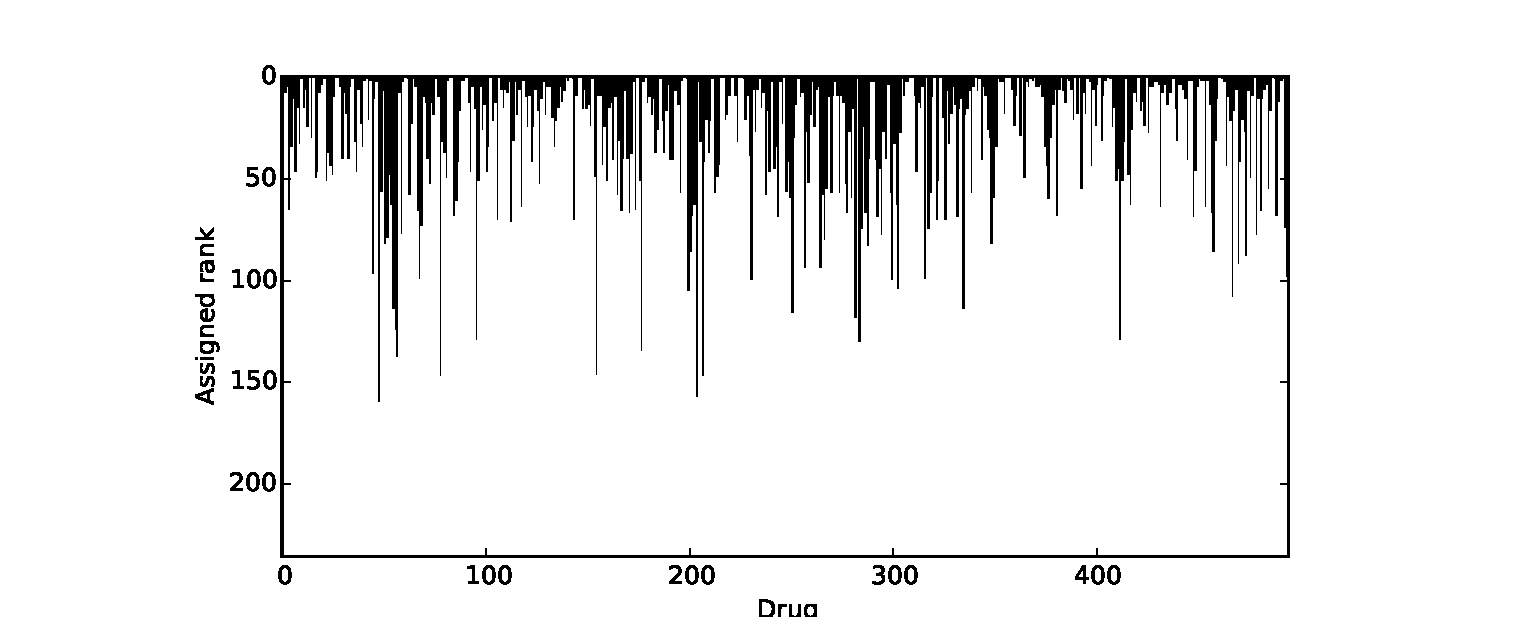
\includegraphics[width=\textwidth]{ref-ctd-heatmap.eps}
\caption{Reference CTD ``heatmap" based on completely correct predictions: black squares are pathways that are actually affected by a given drug. In this case, all such pathways are ranked higher than the unaffected pathways.}
\label{fig:ref-ctd-heatmap}
\end{figure}

To exactly quantify the performance of the model from such an image, metrics like precision and recall are used in information retrieval. 

Imagine covering all but the first line of the aforementioned ``heatmap" and then calculating the fraction of correctly predicted pathways that are visible (black squares) over all ``retrieved" pathways (all visible squares). This is the precision at that rank cutoff. The recall is defined as the fraction of correctly predicted pathways over all correct pathways (including the invisible ones, so the denominator is fixed for this dataset). Naturally, as more and more ranks get uncovered, the recall increases (since we're seeing more and more black squares), whereas the precision can vary (if all the newly uncovered squares are black, it will increase and if they are all white, it will decrease).

In the end of this process, multiple pairs of precision-recall values will be calculated and they can be used to plot a precision-recall curve.

One minor issue with this type of evaluation is that we essentially discard information by ranking pathways, since multiple distributions of pathways can map to the same ranking. In addition, we might prefer a pathway distribution where pathways that are not actually affected by the drug have lower expression values to the one where they are higher. For example, if a drug affects pathways 1 and 2 but not 3, and two models assign to this drug distributions $(0.4, 0.4, 0.2)$ and $(0.5, 0.4, 0.1)$, respectively, then the resultant pathway rankings are the same, but, intuitively, the second model seems to have made a better prediction in this case, since it assigned less probability to the wrong pathway 3.

This intuition can be captured in the following measure:

\begin{equation}
c_d = \sum\limits_{p \in \mathit{ref}_d}{\theta_{d, p}}
\end{equation}

where $\mathit{ref}_d$ is a set of correct pathways for drug $d$ and $\theta_d$ is the predicted pathway distribution for drug $d$. Here, we find the proportion of activity that the model assigned to the pathways that are actually affected by the drug.

One question about this measure is whether we need to take into account the number of pathways the drug actually affects. In the most extreme example, if a drug affects all pathways in the dataset, any model will score a $1.0$ with this measure and so a model that scores 1.0 isn't necessarily ``good". On the other hand, if a drug only affects a single pathway and a model manages to assign $1.0$ to that pathway only, then the model's performance is impressive yet it scores $1.0$, as much as the previous case.

This is the reason comparison with random guessing is important: a random pathway distribution can be generated by drawing $K$ values from a uniform distribution and normalising them. On average, such a distribution will score $\rho_d$ on drug $d$, where $\rho_d$ is the drug's density (the fraction of pathways it actually affects). Hence, we can normalise the measure by dividing it by $\rho_d$ to find out by how much the model did better compared to random guessing. Furthermore, we can take the logarithm of this ratio so that the performance of random guessing ends up at 0, that of anything better than random gets a positive score and the performance of worse than random guessing becomes negative:

\begin{equation}\label{eq:rho-normalised-score}
M_d = \log(\frac{\sum\limits_{p \in \mathit{ref}_d}{\theta_{d, p}}}{\rho_d})
\end{equation}

This value will be referred as the rho-normalised log score further in the analysis.

\chapter{Evaluation}

\section{Toy datasets}

The following subsections describe the datasets which were generated and describes the results of the evaluation as per the aforementioned methods.

\subsection{Description of toy datasets}

The datasets were generated so that they mimic the properties of the real world KEGG/CMap dataset. All datasets have the following in common:

\begin{itemize}[noitemsep]
\item Vocabulary length (number of genes): 3000
\item Number of documents (drugs): 500
\item Number of words in each document: 1000
\item Density of $\beta$: 0.0138
\item Density of $\theta$: 0.1231
\end{itemize}

Densities here refer to the fraction of non-zero elements in each matrix. The KEGG/CMap dataset is very sparse: each pathway only affects, on average 1.38\% of all genes and each drug only affects, on average, 12.3\% of all pathways. The density value for $\beta$ was calculated by taking the matrix of priors (since it explicitly enforces the pattern of zeros in the result), whereas the density value for $\theta$ was calculated by taking the reference (CTD) dataset.

The first four datasets allow to investigate how the performance of the model changes when the number of topics increases:

\begin{itemize}[noitemsep]
\item Dataset 1: 10 topics
\item Dataset 2: 20 topics
\item Dataset 3: 50 topics
\item Dataset 4: 100 topics
\end{itemize}

The parameters of the fifth dataset were designed to mimic the real-world one as closely as possible in order to determine, by comparing the performance of the model on that dataset against the real-world one, whether the drug gene expression data follows the generative framework described by the CTM. In addition to reusing all the parameters the first 4 datasets were generated with, for this dataset I also approximated the $\mu$ and $\Sigma$ of the reference by first calculating the topic distribution $\theta$ implied by the dataset (assuming all pathways in the resultant matrix are equally weighted) and then calculating the mean and the covariance matrix of the distribution of pathways based on it.

In the last 4 datasets, the number of topics was kept at 20 and I varied the density of the covariance matrix: the proportion of pathways in the implied matrix of correlations that are connected:

\begin{itemize}[noitemsep]
\item Dataset 6: No correlations: use the identity matrix as $\Sigma$
\item Dataset 7: Density 10\%
\item Dataset 8: Density 50\%
\item Dataset 9: Density 90\%
\end{itemize}

\subsection{Overall analysis}

\begin{figure}[!htb]
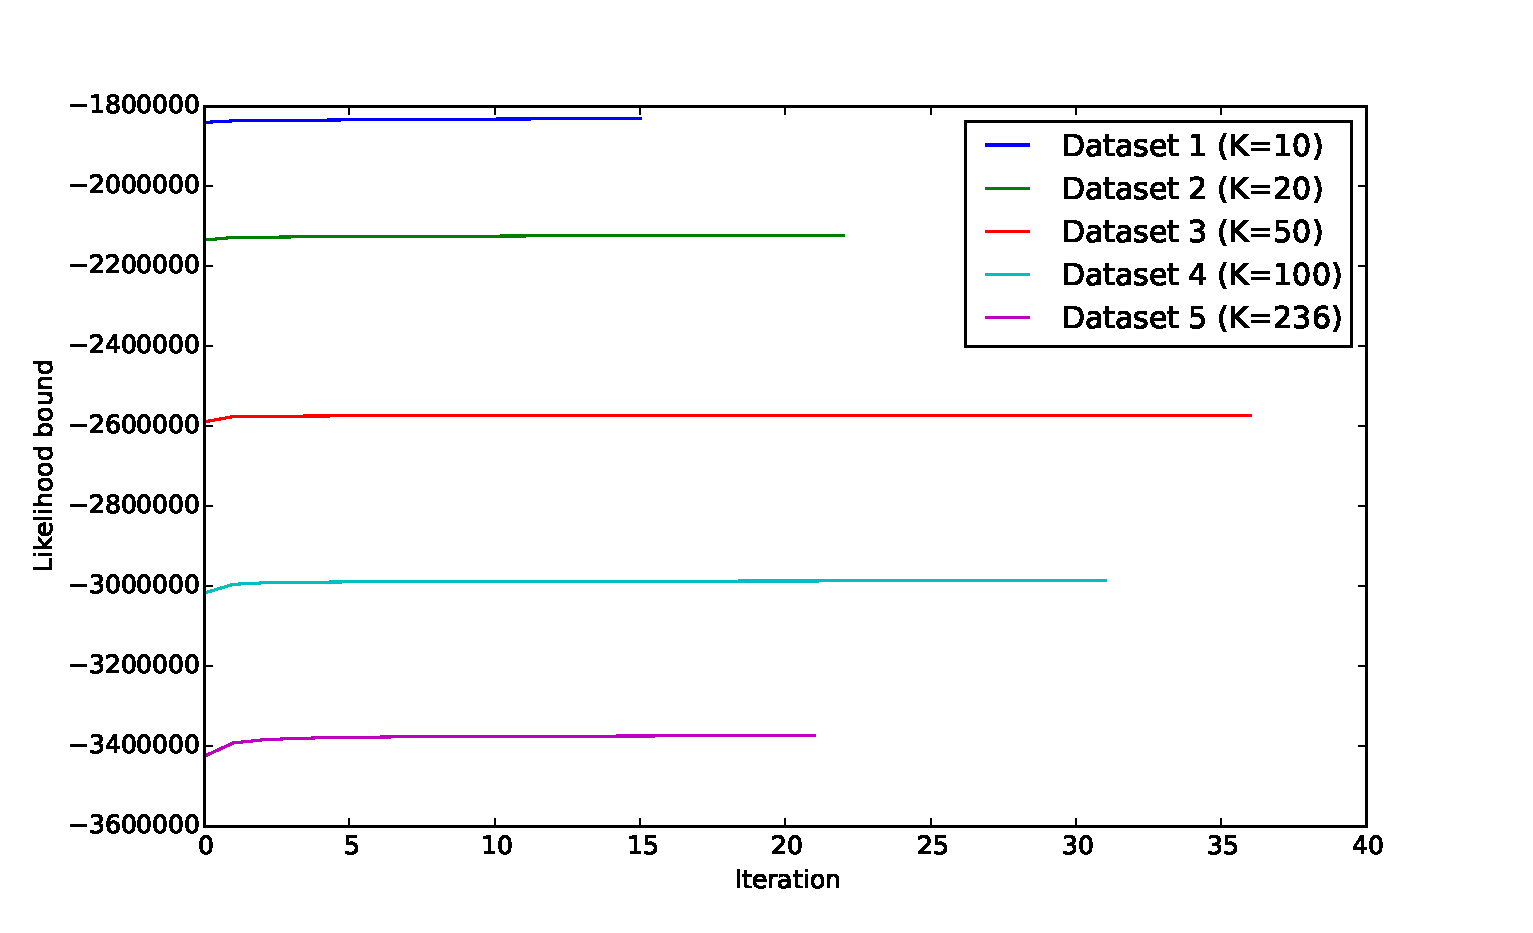
\includegraphics[width=\textwidth]{sim-likelihood-bounds-1-5.eps}
\caption{Likelihood bound on the corpus reported by the CTM on the toy datasets with different numbers of topics}
\label{fig:sim-likelihood-bounds-1-5}
\end{figure}

\begin{figure}[!htb]
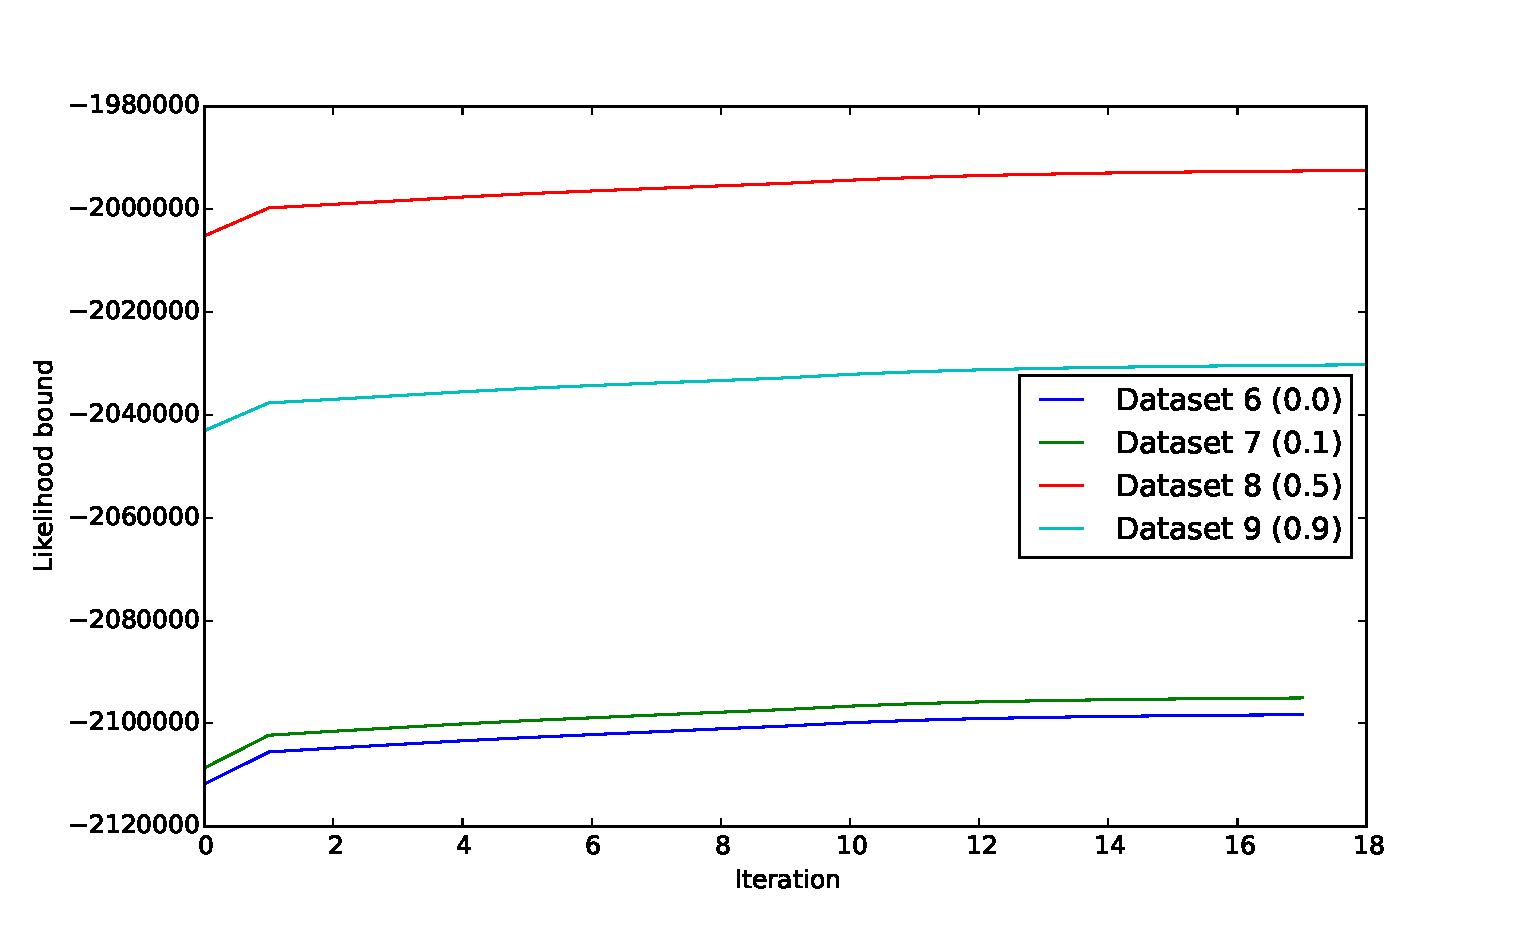
\includegraphics[width=\textwidth]{sim-likelihood-bounds-6-9.eps}
\caption{Likelihood bound on the corpus reported by the CTM on the toy datasets with different densities of the correlation matrix (in brackets in the legend)}
\label{fig:sim-likelihood-bounds-6-9}
\end{figure}

At every iteration, the model outputs a likelihood bound that it assigns to the data and continues updating the model parameters until the likelihood bound converges (the change is less than a certain threshold, $2\times10^{-5}$ in this case). The likelihood bound values over iterations are plotted on figures~\ref{fig:sim-likelihood-bounds-1-5}~and~\ref{fig:sim-likelihood-bounds-6-9}. Increasing the number of topics the corpus was generated with decreases the likelihood bound but doesn't seem to be in a direct relationship with the rate of convergence (the number of iterations).

\begin{figure}[!htb]
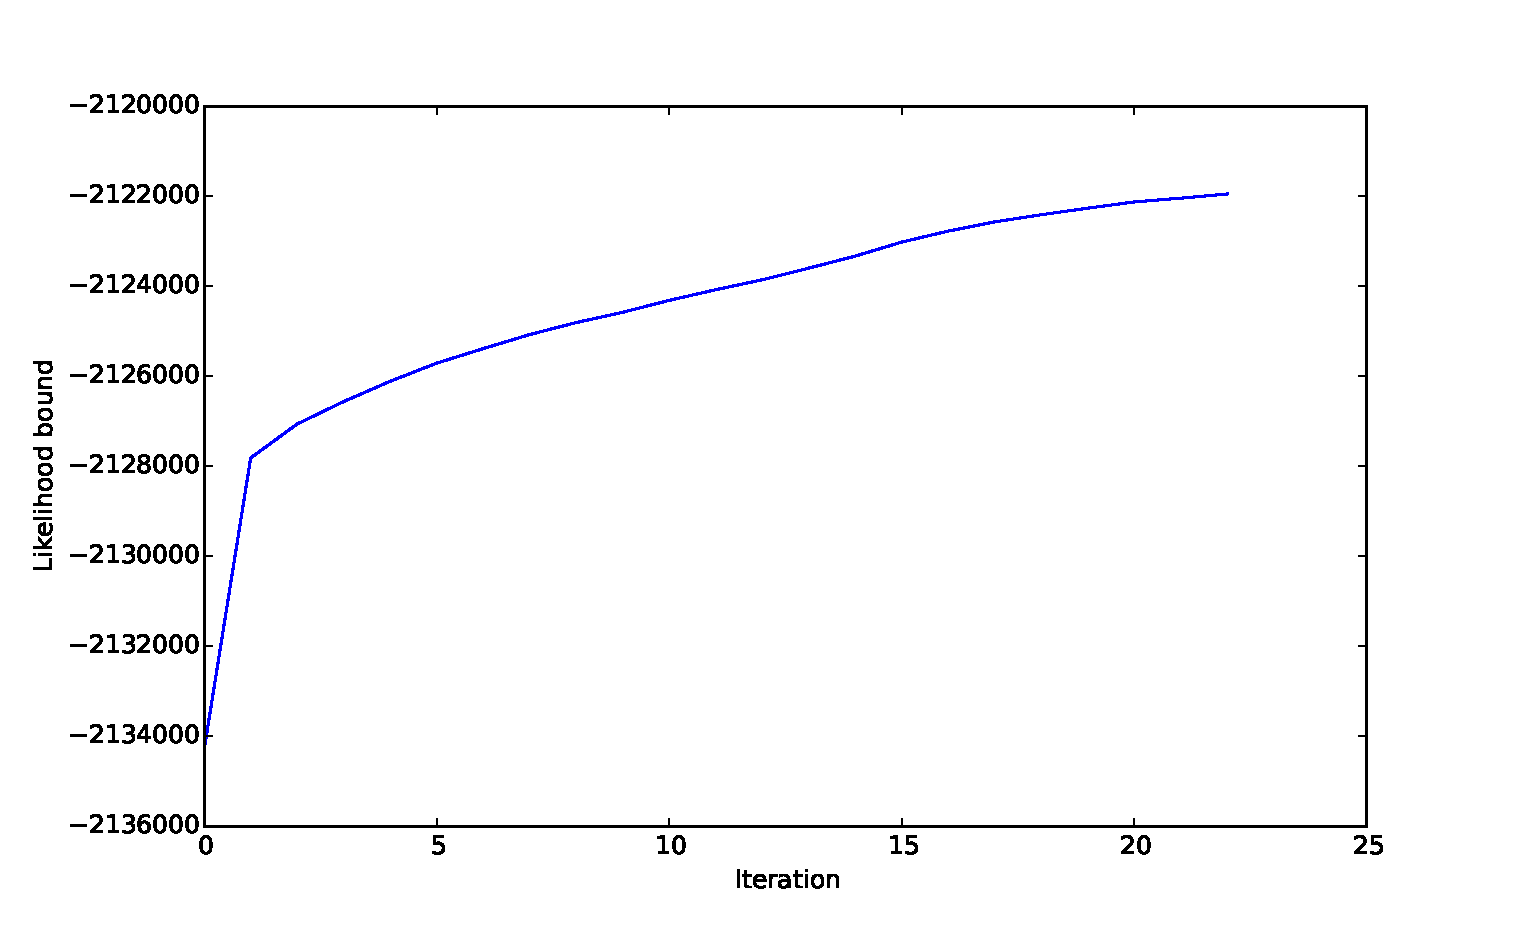
\includegraphics[width=\textwidth]{sim-likelihood-bounds-k-20.eps}
\caption{Likelihood bound on dataset 2 (20 topics) reported by the CTM as the training progresses}
\label{fig:sim-likelihood-bounds-k-20}
\end{figure}

The difference between bounds is large enough for it to be difficult to see the general shape of the likelihood bound curve. Figure~\ref{fig:sim-likelihood-bounds-k-20} plots the sample likelihood bound curve for one of the toy datasets. The training essentially follows a power law: most of the progress happens in the first few iterations.

Overall, the model achieves great performance on the prediction of the distributions of topics the document was generated with. It would hence be reasonable to assume that if the model predicts the topic distribution for a document consistently well, it will also be able to recover the model parameters the corpus was generated with, since this is what the model relies on for its predictions. However, this is not exactly the case: the model's ability to recover the parameters ($\mu, \Sigma, \beta$) degrades quickly beyond that of random guessing as the number of topics increases. The reasons for this will be discussed further.

In addition, since the output of every iteration of training are only the refined model parameters and even after convergence these model parameters are far away from the real parameters, it could be the case that further iterations do not improve the quality of prediction of the topic distributions. Hence, the performance of 1-iteration CTM is also investigated in attempts to see whether the lengthy CTM training process can be shortened.

\subsection{Topic prediction}

\begin{figure}[!htb]
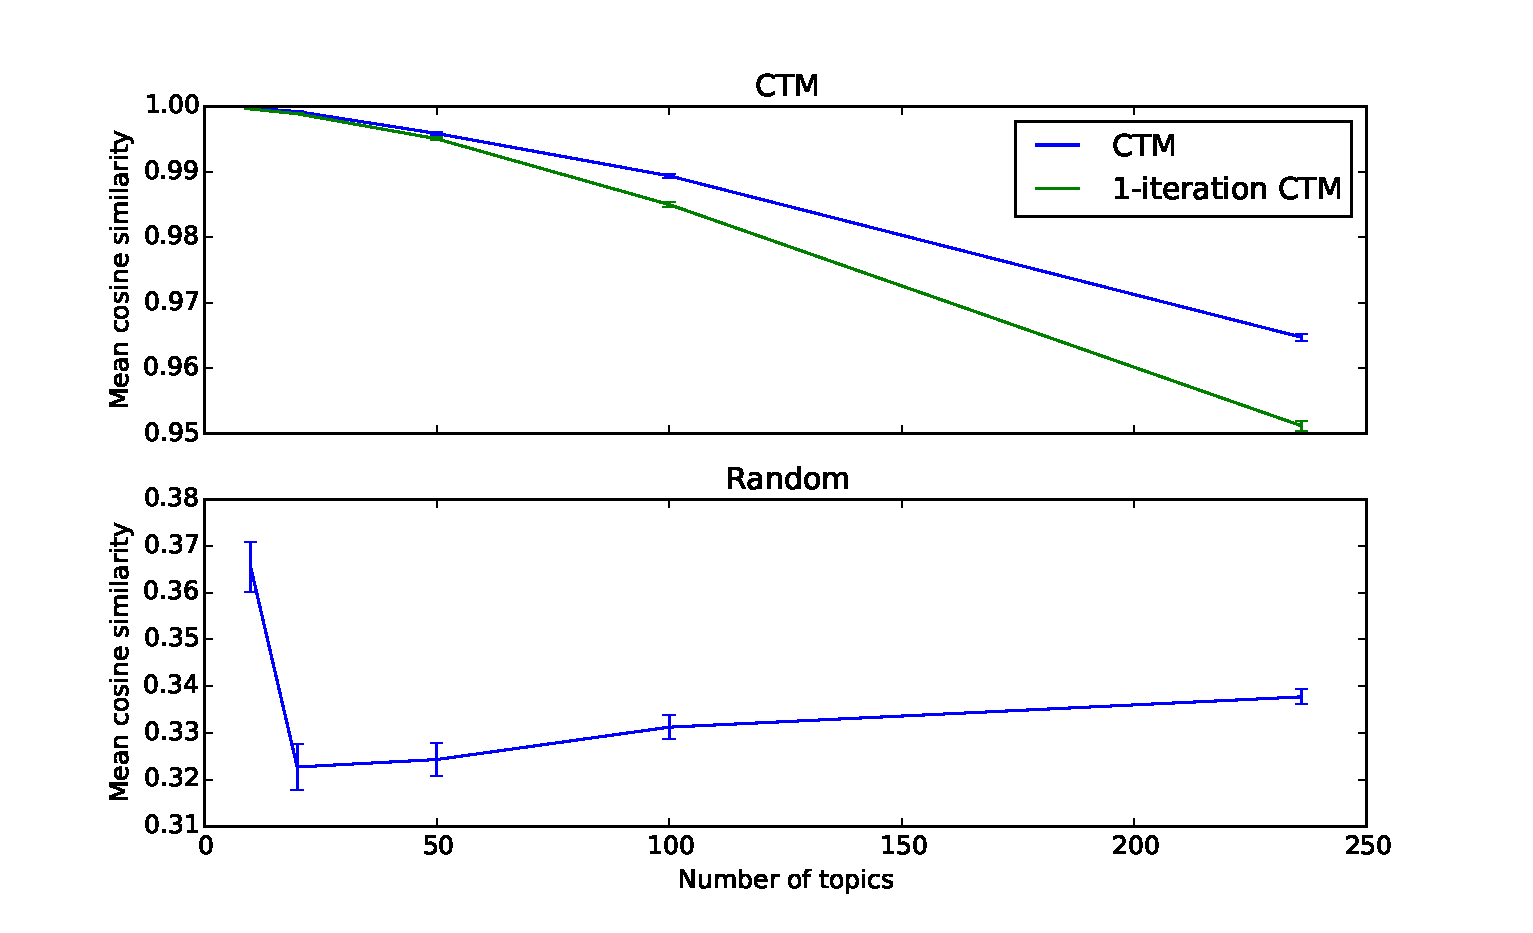
\includegraphics[width=\textwidth]{sim-cosine.eps}
\caption{The mean cosine similarity between inferred and reference document-topic distributions $\theta$ as a function of the number of topics in the toy datasets}
\label{fig:sim-cosine}
\end{figure}

Figure~\ref{fig:sim-cosine} shows the mean cosine similarity between each $\theta_d$ in the inferred and the reference dataset. It can be seen that both CTM and 1-iteration CTM vastly outperform random guessing on all numbers of topics, but their performance degrades as the number of topics increases. Furthermore, the 1-iteration CTM is consistently worse than the full CTM, but not by much: it can still provide a good approximation to the CTM in a fraction of the required training time.

\begin{figure}[!htb]
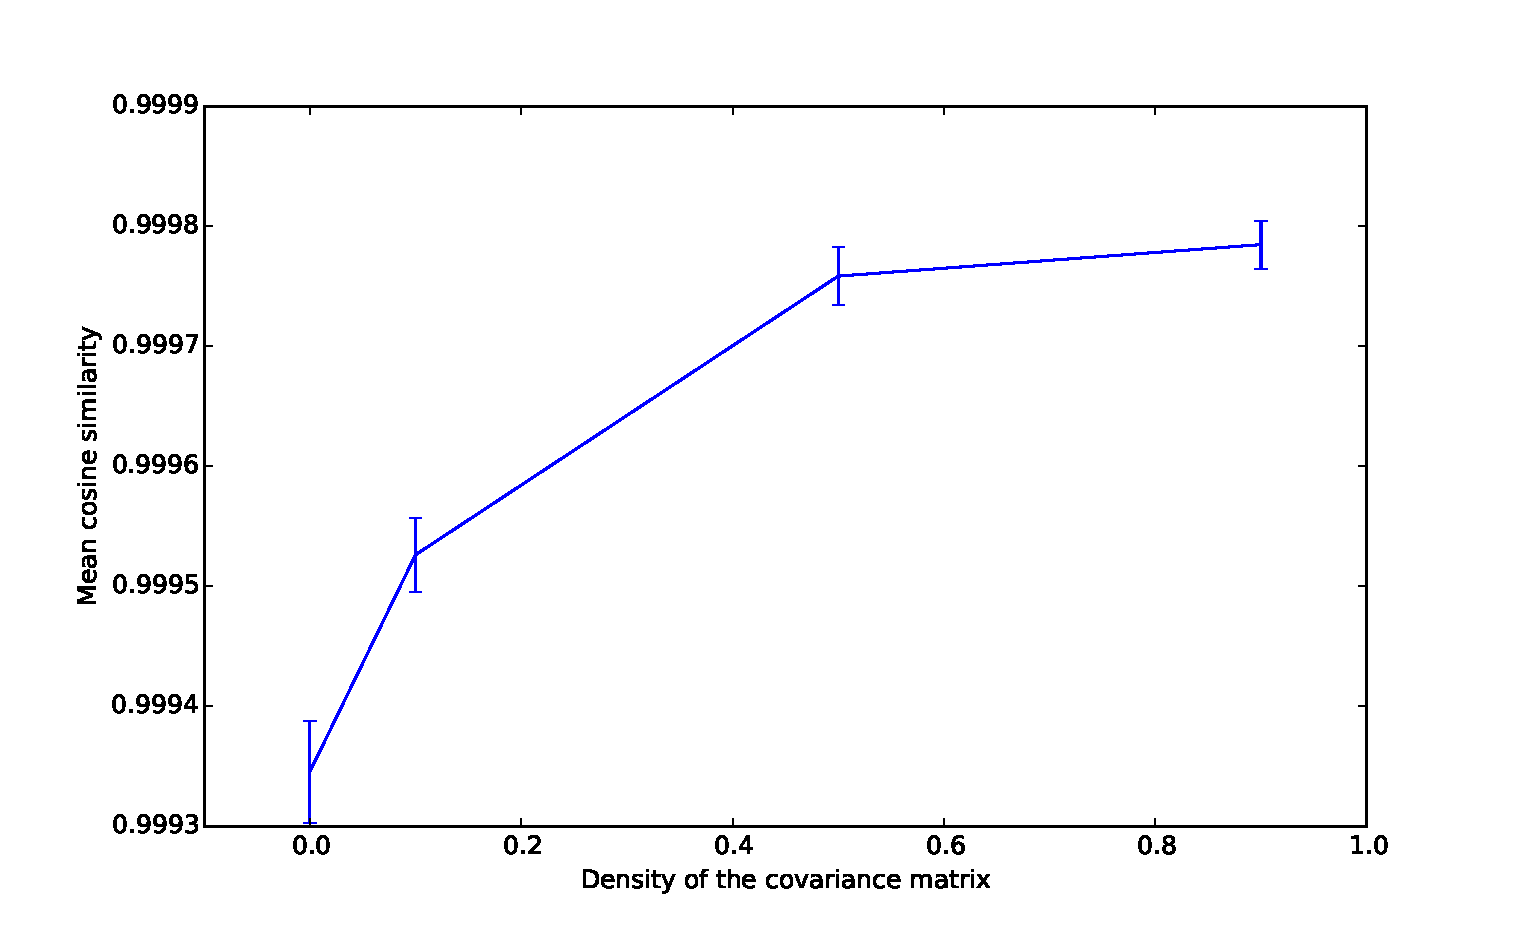
\includegraphics[width=\textwidth]{sim-sigmadensity-cosine.eps}
\caption{The mean cosine similarity between inferred and reference document-topic distributions $\theta$ as a function of the density of the global topic covariance matrix $\Sigma$}
\label{fig:sim-sigmadensity-cosine}
\end{figure}

Figure~\ref{fig:sim-sigmadensity-cosine}, on the other hand, shows how the performance of CTM changes as the 20 topics in the toy dataset become more correlated. True to its name, the Correlated Topic Model benefits from more correlated topics.

\subsection{Parameter recovery}

\begin{figure}[!htb]
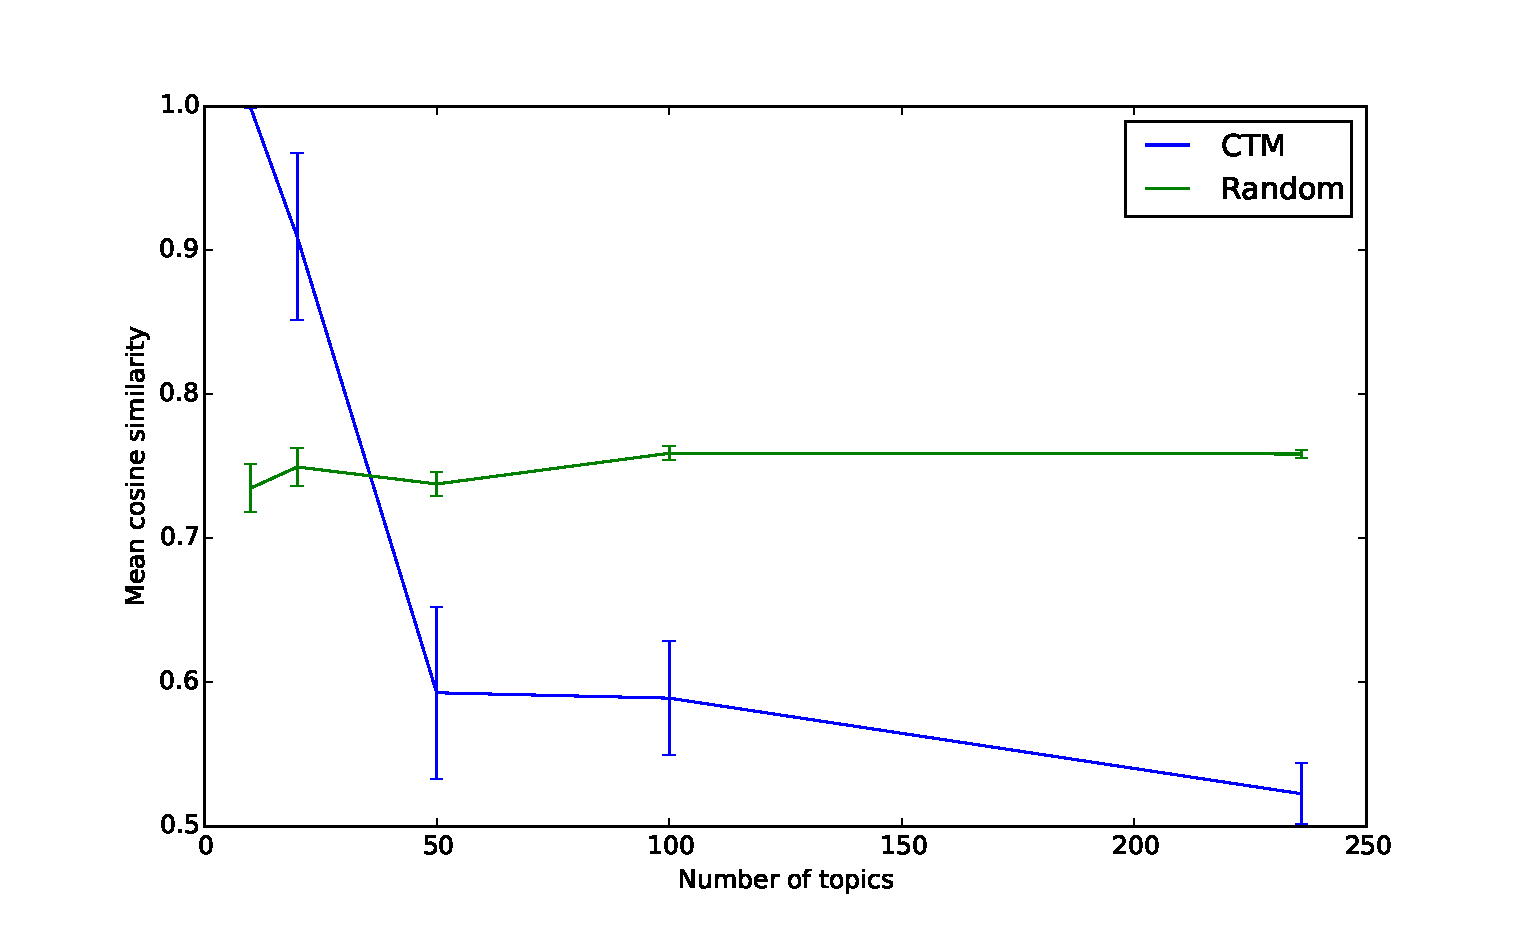
\includegraphics[width=\textwidth]{sim-beta-cosine.eps}
\caption{Cosine similarities between the inferred and reference topic-word distributions as a function of the number of topics in the toy datasets}
\label{fig:sim-beta-cosine}
\end{figure}

\begin{figure}[!htb]
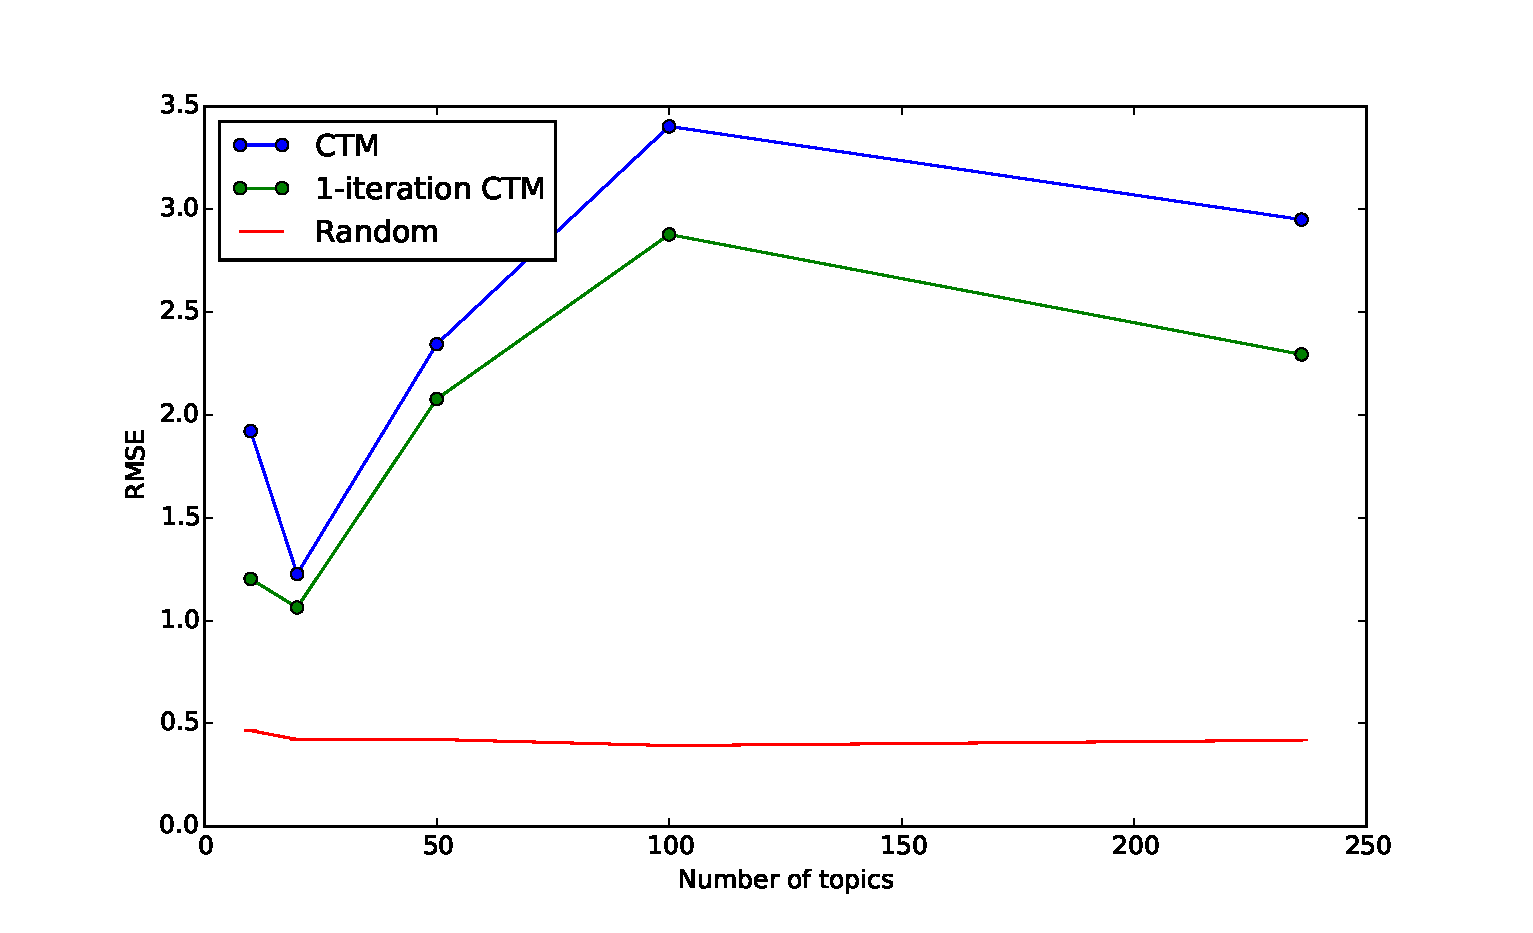
\includegraphics[width=\textwidth]{sim-mu-rmse.eps}
\caption{Normalised RMSE between inferred and reference $\mu$ as a function of the number of topics}
\label{fig:sim-mu-rmse}
\end{figure}

\begin{figure}[!htb]
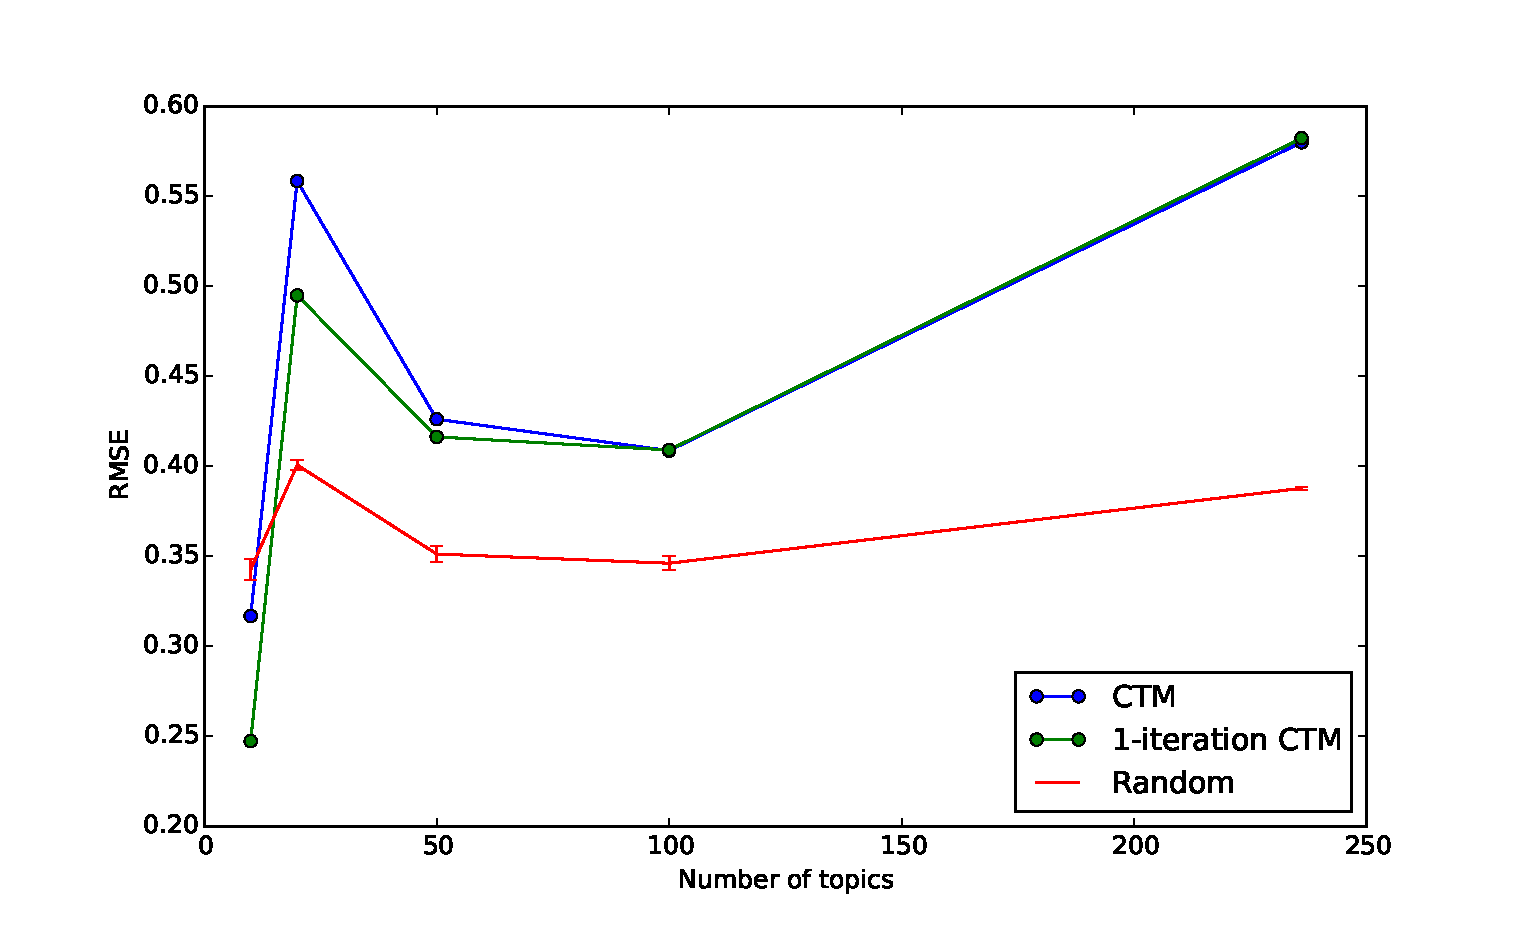
\includegraphics[width=\textwidth]{sim-sigma-rmse.eps}
\caption{Normalised RMSE between inferred and reference $\Sigma$ as a function of the number of topics}
\label{fig:sim-sigma-rmse}
\end{figure}

Figure~\ref{fig:sim-beta-cosine} shows the mean cosine similarity between the inferred and the reference rows of the $\beta$ matrix (the word distributions for every topic). There are $K$ topics in a single dataset and so every data point on this graph has been obtained by averaging the cosine similarities across $K$ samples. The random topic-word matrices here were generated by taking the Boolean matrix of priors and replacing the ``1" values with a draw from a uniform distribution and then renormalising.

As evident from the figure, the recovery of the topic-word matrix gets much worse as the number of topics increases and becomes further away from the reference than a random topic-word matrix after the third dataset. The reason for this is that the pattern of zeros in the resultant matrix differs from the matrix of priors even though the priors have been enforced. If the prior matrix contains a zero in a certain position, the inferred matrix is guaranteed to have a zero in the same position as well, since the zeros propagate through the training process. However, this doesn't mean that a zero in a certain position in the inferred matrix is also in the reference matrix. It appears that the training process can introduce a zero in certain positions and it will stay there throughout the remaining training iterations. This appears to be an issue of the topic recoverability and prior enforcement.

Another problem is the poor recoverability of the parameters of the global topic distribution, $\mu$ and $\Sigma$ (Figures~\ref{fig:sim-mu-rmse}~and~\ref{fig:sim-sigma-rmse}, smaller RMSE is better). The performance of random guessing of was found by taking 1000 samples for $\mu$ and 100 samples for $\Sigma$.

The issue here is that every sample $\theta$ from $N(\mu, \Sigma)$ is altered after sampling by enforcing a certain number of zero elements. Hence, the document-topic distributions after generation are not guaranteed to follow a normal distribution with the original parameters.

For example, consider two drawn $\theta_1 = (\theta_{1,1}, \theta_{1,2}, \theta_{1,3}), \theta_2 = (\theta_{2,1}, \theta_{2,2}, \theta_{2,3})$. After the zero enforcement, these two vectors could become $\theta'_1 = (\theta_{1,1}, 0, 0), \theta'_2 = (\theta_{2,1}, 0, \theta_{2,3})$ (unnormalised). They are now more similar than they were (since the second positions have both been set to zero), which introduces a bias into the correlations.

\begin{figure}[!htb]
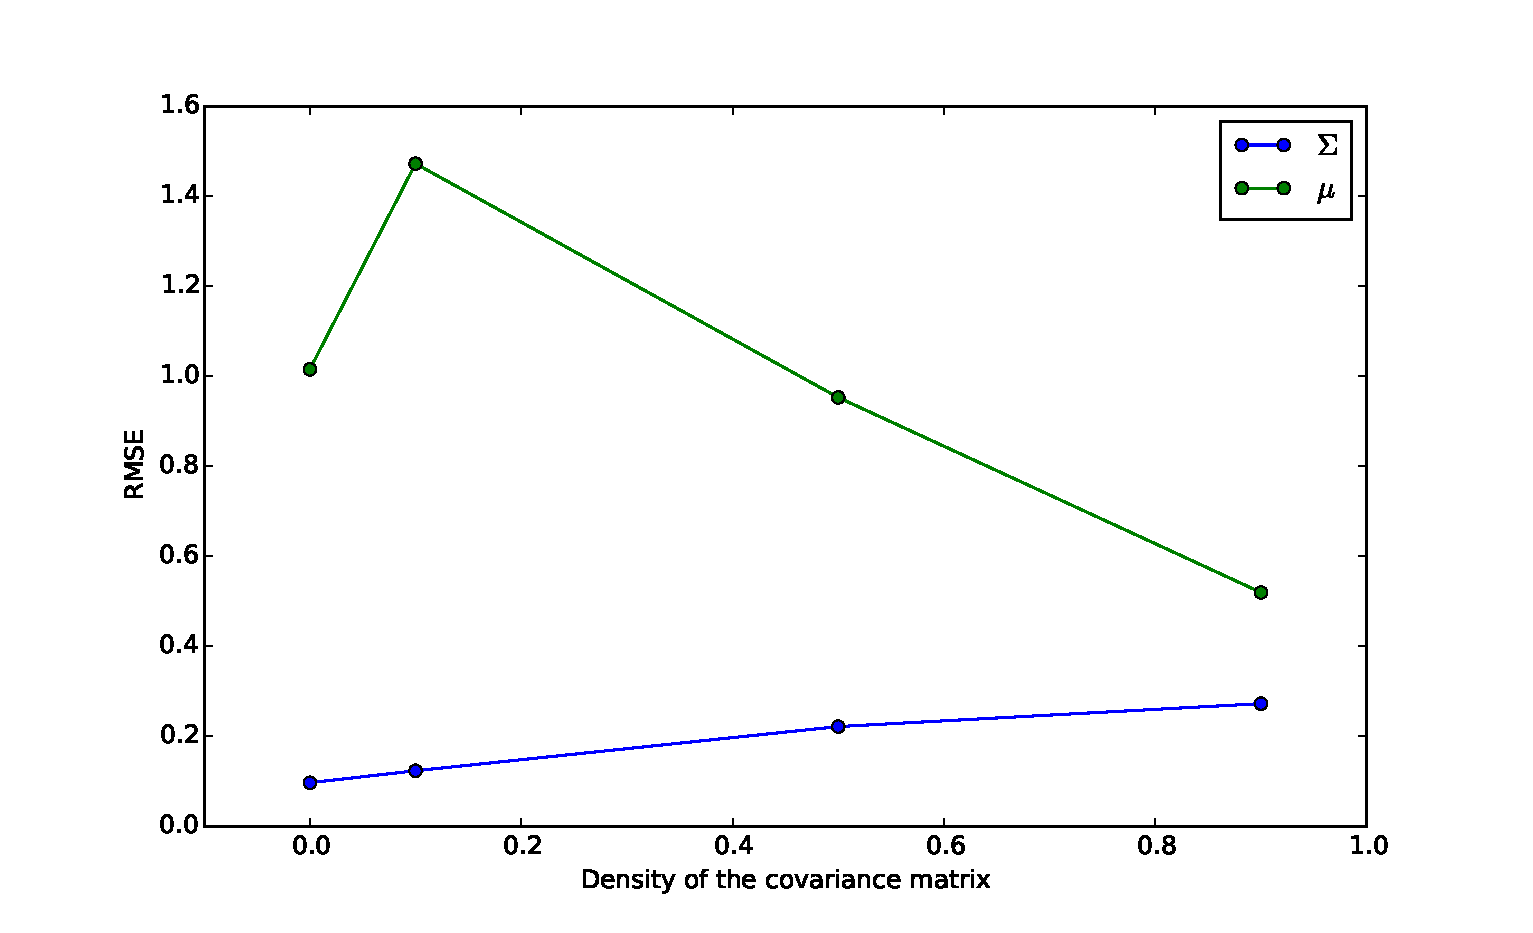
\includegraphics[width=\textwidth]{sim-sigmadensity-musigma.eps}
\caption{Normalised RMSE between inferred and reference $\mu$ and $\Sigma$ as a function of the density of the global topic covariance matrix $\Sigma$}
\label{fig:sim-sigmadensity-musigma}
\end{figure}

\begin{figure}[!htb]
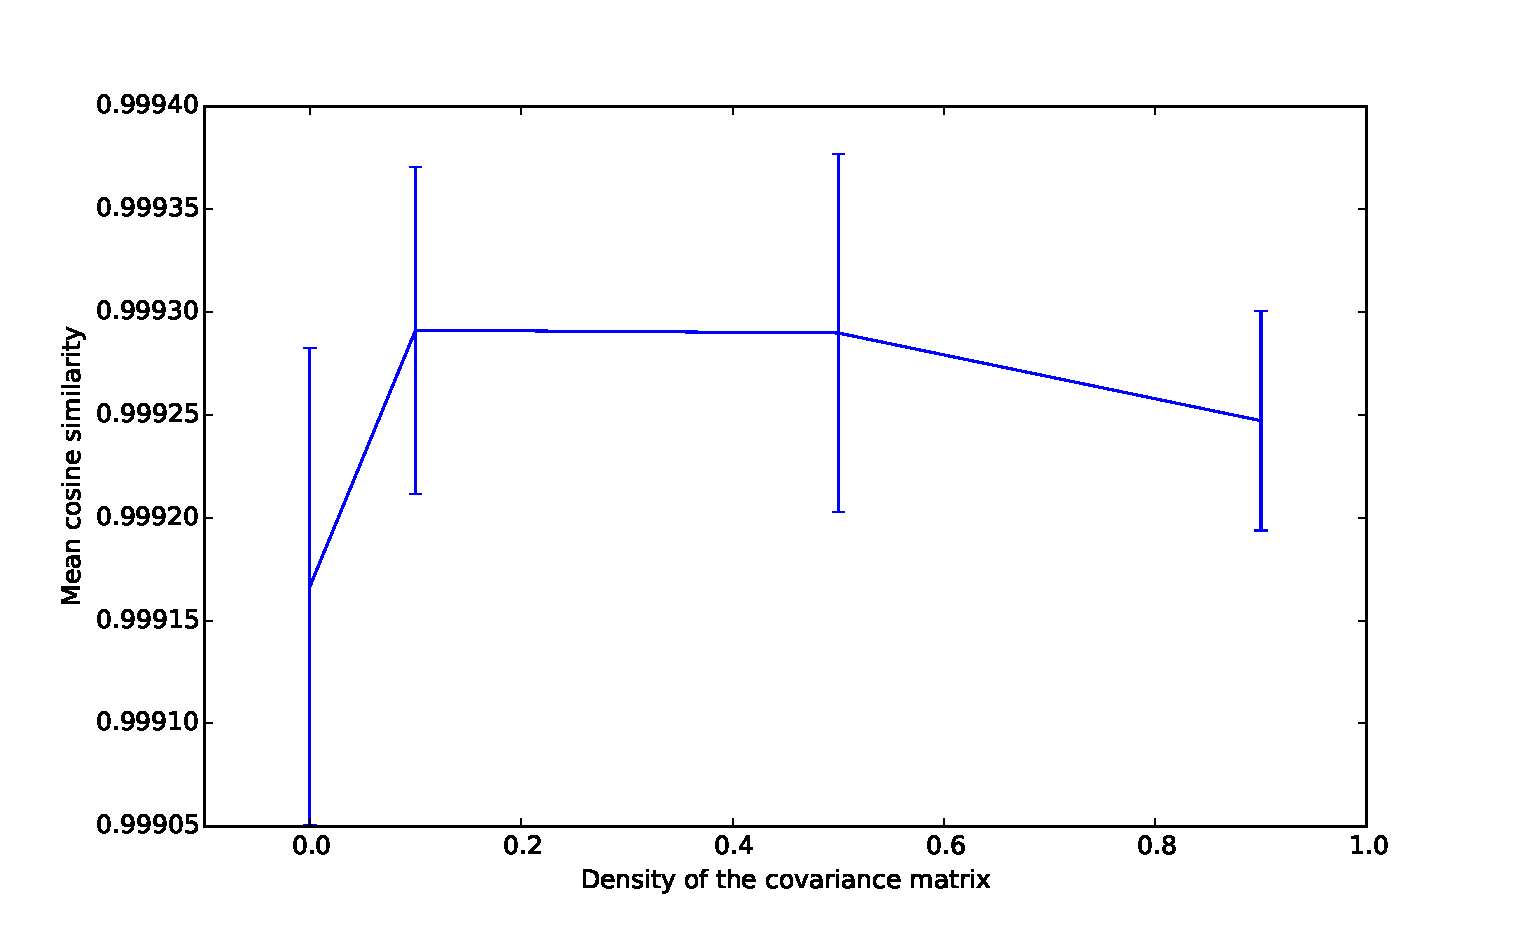
\includegraphics[width=\textwidth]{sim-sigmadensity-beta.eps}
\caption{Cosime similarities between the inferred and reference topic-word distributions $\beta$ as a function of the density of the global topic covariance matrix $\Sigma$}
\label{fig:sim-sigmadensity-beta}
\end{figure}

Figure~\ref{fig:sim-sigmadensity-musigma} shows that as topics become more correlated, the recovery performance for $\mu$ dramatically improves, whereas the recovery of $\Sigma$ itself becomes worse. However, the recovery performance of $\beta$ doesn't significantly change with the correlation density (Figure~\ref{fig:sim-sigmadensity-beta}).

TODO: performance for beta and sigma here seems to be better than for K=20 in the topic number study (mu is fine, around 1.0), the only difference being that the sigma had enforced densities in this case; beta mean cosine similarity has a strong correlation to the standard deviation of the diagonal of the covariance matrix (``deviation of deviations", so the proportions are more varied), but sigma RMSE doesn't, maybe something to do with the values of the matrix? shouldn't affect the correlation matrix

\subsection{Rank recovery}

\begin{figure}[!htb]
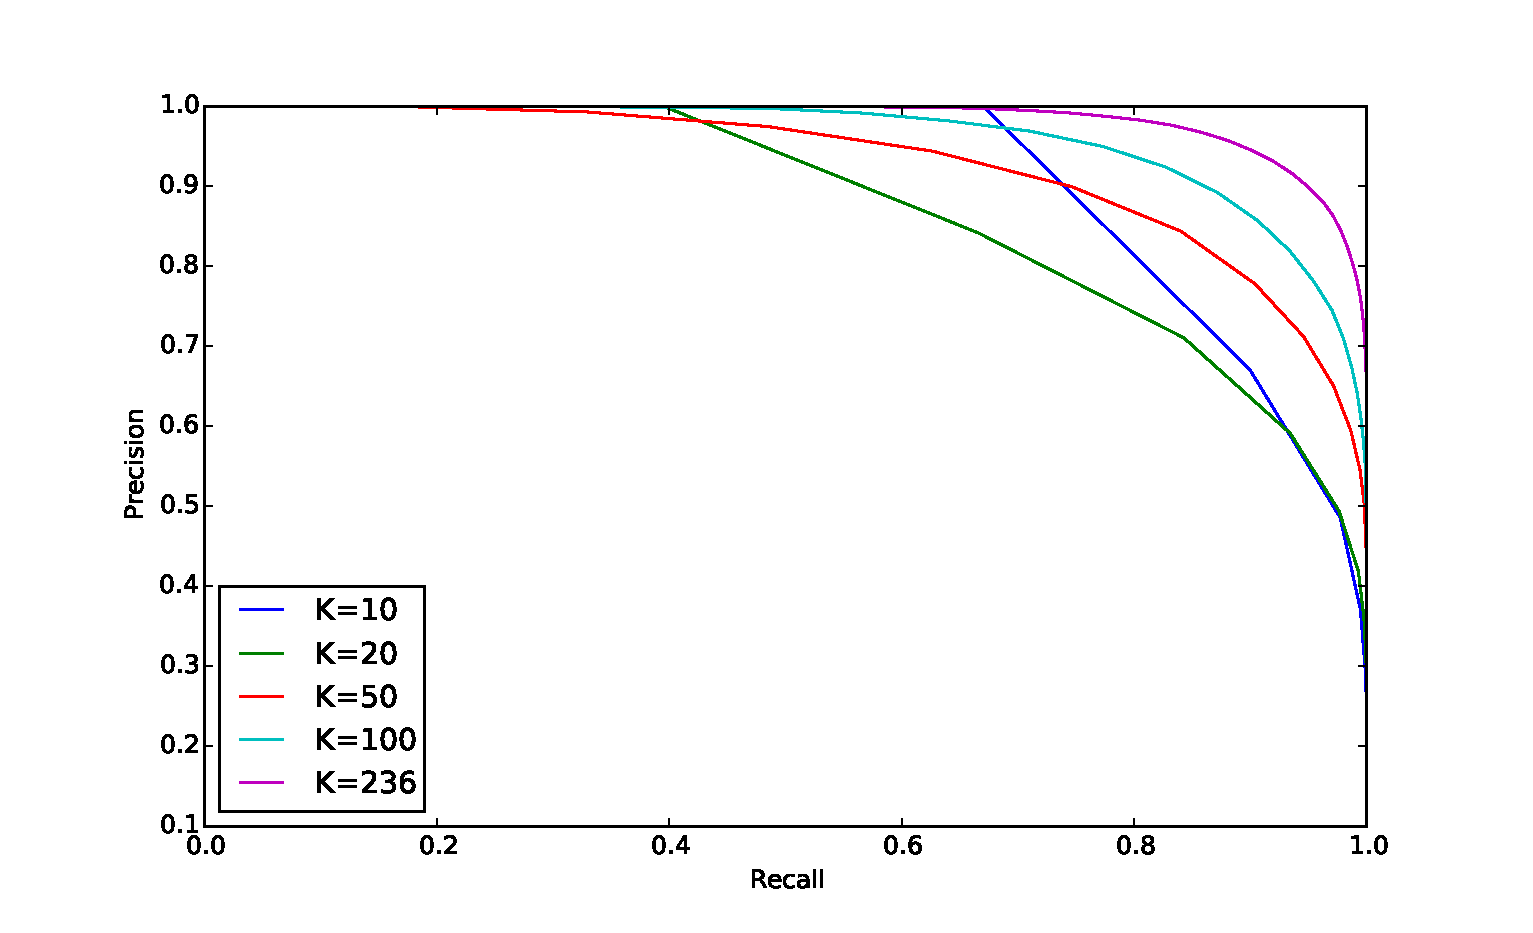
\includegraphics[width=\textwidth]{sim-pr-curves-all.eps}
\caption{Precision-recall curves for CTM on the toy datasets}
\label{fig:sim-pr-curves-all}
\end{figure}

Figure~\ref{fig:sim-pr-curves-all} shows the precision-recall curves for the toy datasets with different number of topics on the same axis. The reference precision-recall curves (where all relevant topics/pathways are in the top ranks) can also be plotted, but in this case the CTM curves are so close to the reference curves they are indistinguishable. The precision-recall curves for the 1-iteration CTM also coincide with these curves.

However, according to the previous tests, the topic recovery of CTM is not perfect and the 1-iteration CTM does give slightly different results from the full CTM, so a different method has to be used to evaluate how CTM fares on ranked retrieval tasks.

\begin{figure}[!htb]
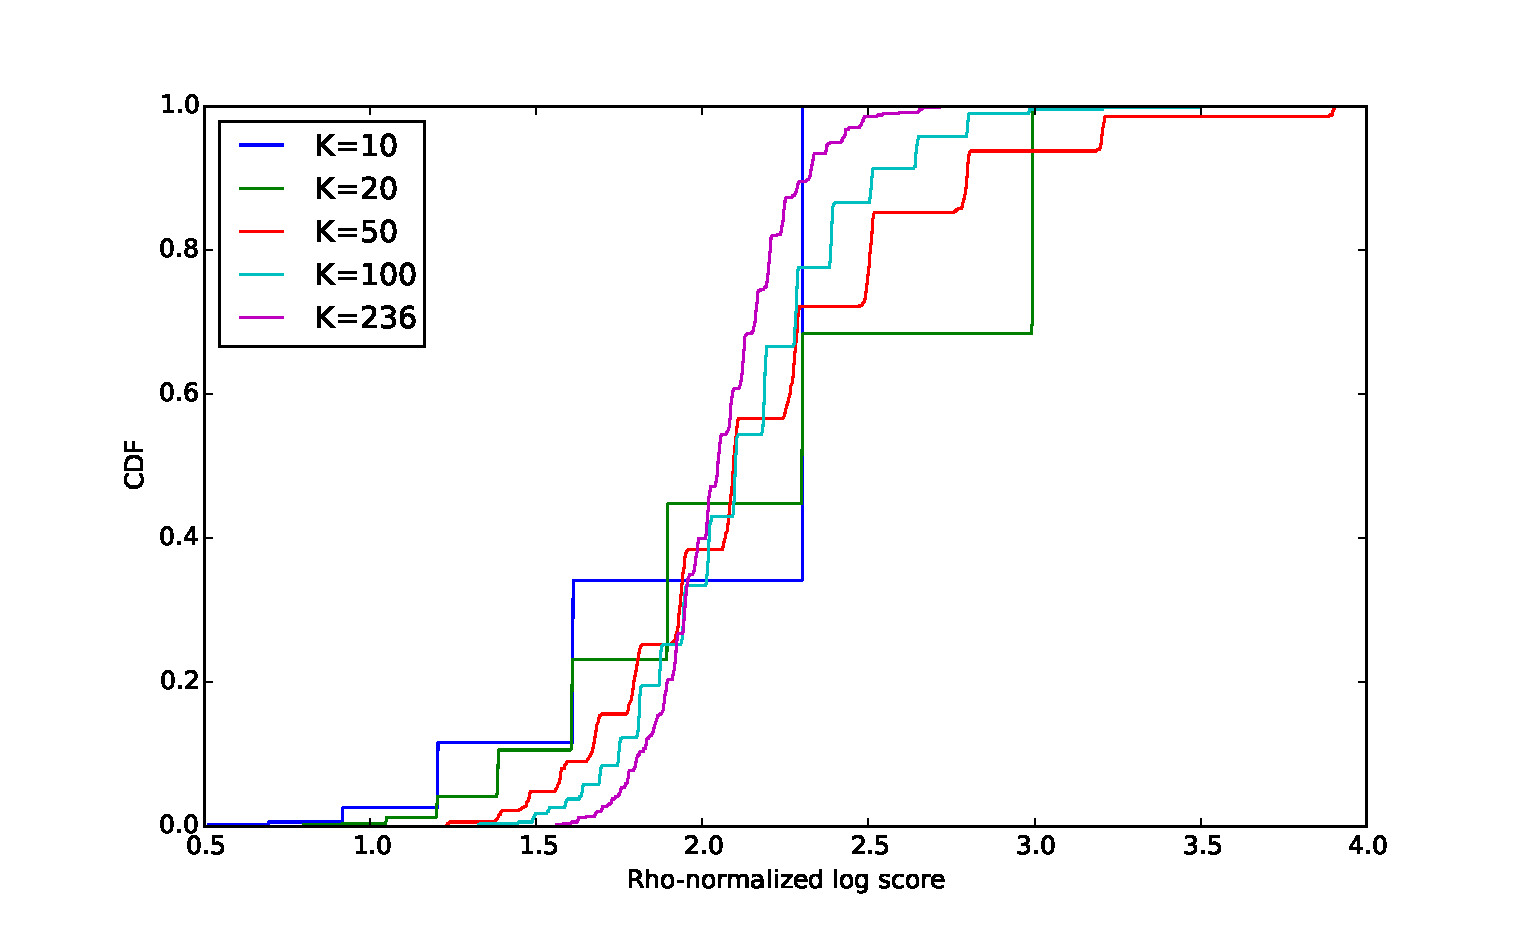
\includegraphics[width=\textwidth]{sim-log.eps}
\caption{Cumulative distribution function (CDF) of the distribution of the rho-normalised log scores of CTM on the toy datasets}
\label{fig:sim-log}
\end{figure}

Figure~\ref{fig:sim-log} shows the cumulative plots (for every value of the score on the horizontal axis, the fraction of the values that are below it) of rho-normalised log scores (Equation~\ref{eq:rho-normalised-score}) as the number of topics changes. While these plots do show that the CTM gives a much better performance than random guessing (since all scores are above 0), the figure is too confusing for any conclusions to be made. It does, however, show an interesting ``staircase" effect where the scores fall into discrete bins whose amount increases with the number of topics. This is because the unnormalised measure (sum of inferred expression levels for correct pathways) is close to 1 and so the final score only depends on the normalisation factor, which only depends on the number of pathways the drug actually has.

\begin{figure}[!htb]
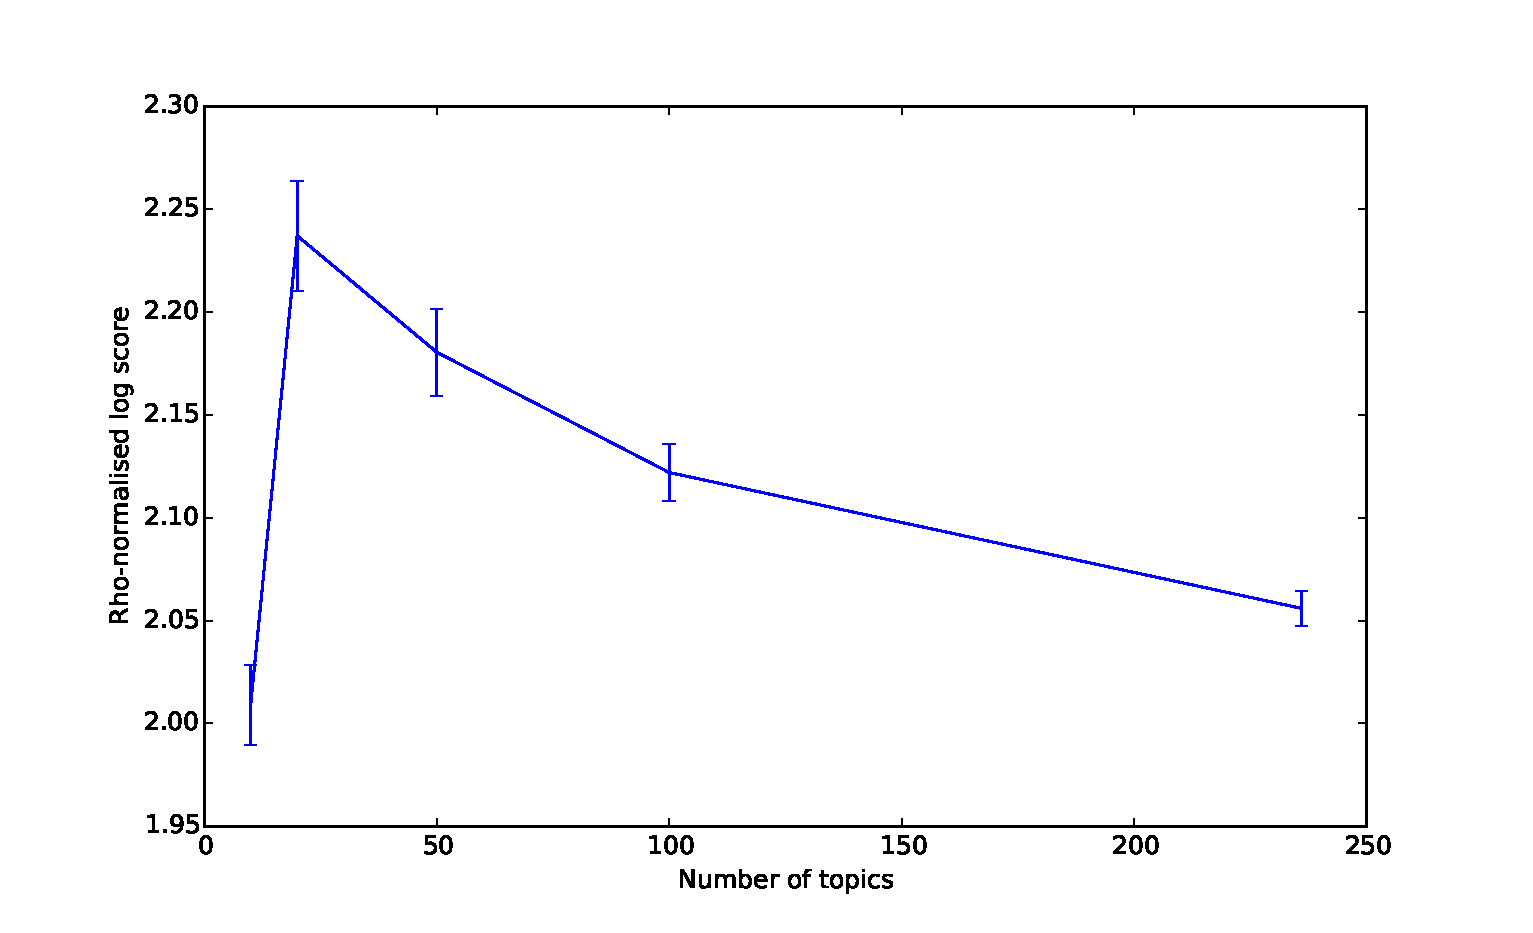
\includegraphics[width=\textwidth]{sim-average-rho.eps}
\caption{Mean rho-normalised log score as a function of the number of topics in the toy datasets}
\label{fig:sim-average-rho}
\end{figure}

Figure~\ref{fig:sim-average-rho} shows the mean score the model achieved on every dataset, plotted against the number of topics. The performance of the model generally degrades with the number of topics, however there is a peak somewhere between $K=10$ and $K=50$ where the model achieves top performance. Doing just one iteration of CTM brings its scores very close to those of CTM, though they diverge as the number of topics increases.

\begin{figure}[!htb]
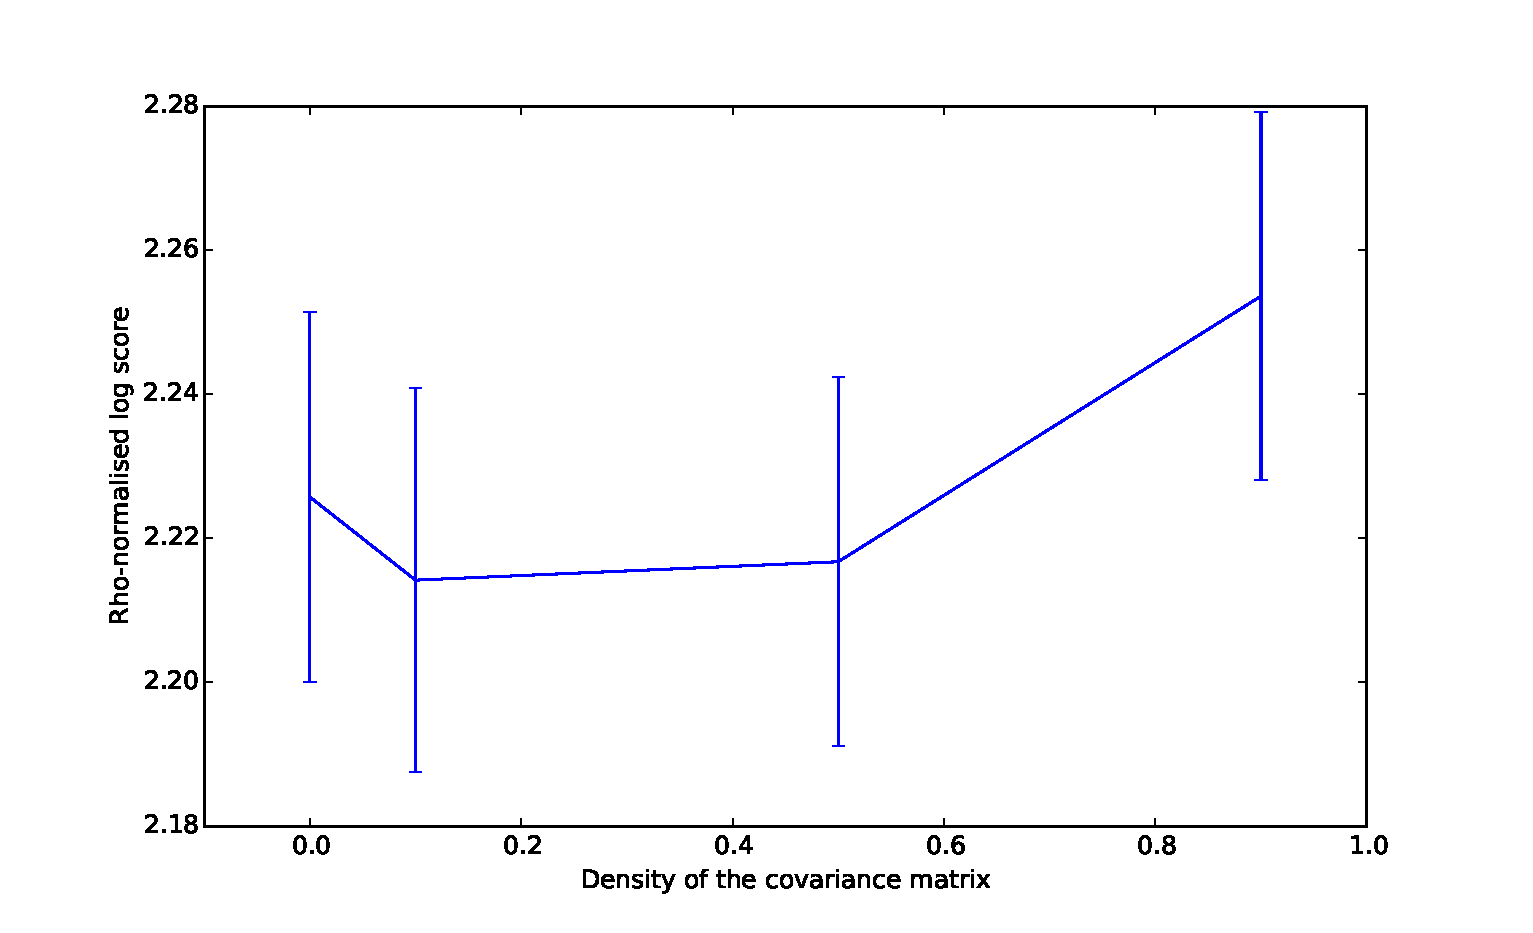
\includegraphics[width=\textwidth]{sim-sigmadensity-rho.eps}
\caption{Mean rho-normalised log score of CTM on the toy datasets as a function of the density of the global topic covariance matrix $\Sigma$}
\label{fig:sim-sigmadensity-rho}
\end{figure}

Figure~\ref{fig:sim-sigmadensity-rho} shows how the mean score changes as the topics become more correlated. It appears the performance of CTM does increase with topic correlations in this case, but the variance in performance between different drugs is too large to draw a meaningful conclusion here.

\subsection{Conclusion}

On the datasets of similar characteristics to the real-world KEGG/CMap dataset (large document-topic and topic-word sparsity levels) the CTM achieves great performance in the prediction of the document-topic distributions $\theta_d$, both when the evaluation method uses the reference distributions and when they have been turned into Boolean matrices. On the other hand, enforcing such large sparsity levels on $\theta$, in essence, breaks the assumptions about the generative process of the CTM which the model's training process relies on and the parameter recovery becomes much worse than random guessing.

Furthermore, only performing one training iteration of the CTM, as opposed to training the CTM until its likelihood bound on the corpus converges, result in better recovery performance of $\mu$ and $\beta$ and similar performance for $\Sigma$. The performance on the document-topic distribution recovery is rather close (and still much better than random guessing) but diverges from the full CTM as the number of topics increases.

Hence, if the real-world drug-gene expression data does follow the generative framework assumed by the CTM, the expected results are good topic recovery (good performance on predicting the drug-pathway relationships) and poor recovery of the correlations between pathways and the pathway-gene memberships. Performing only one EM cycle on CTM should improve that, but at the expense of the prediction of the drug-pathway relationships.

\section{KEGG and CMap datasets}

\subsection{Description of the dataset}

KEGG (Kyoto Encyclopedia of Genes and Genomes), published by Kyoto Universiy Katehisa Laboratories, is an online collection of databases dealing with various aspects of biology. Of interest to this project is the KEGG PATHWAY database, a collection of pathways and genes which they include.

CMap (Connectivity Map), published by the Broad Institute is a catalog of gene-expression data.

These two datasets are used to derive the following matrices:

\begin{itemize}[noitemsep]
\item Drug-gene expression matrix, where each entry is the logarithm of the ratio of the expression of the gene when treated with a certain drug against the baseline, rounded to 2 decimal places.
\item Boolean gene-pathway membership matrix that has a ``1" entry if the pathway contains a given gene and ``0" if it doesn't.
\end{itemize}

I used the same preprocessed data that was used in the LDA paper, so I didn't have to perform the preprocessing of the raw gene expression data myself. This was so that the results from the LDA and the CTM method could be compared.

Before the CTM can be trained on the dataset, the drug-gene expression data has to be turned into a sort of a ``document", since we're now operating in terms of words and word counts. Both LDA and my implementation of CTM do it by taking the absolute value of each element and multiplying it by 100 (since the preprocessed data has been rounded to the nearest 0.01). Observe that this discards the sign of the expression value and since we're operating in log space, this means that the gene expression ratios that are reciprocals of each other will be treated the same.

I was not comfortable with this method since it involved discarding information that the model might have had a use for, but the CTM training process does require nonnegative values. I hence performed another experimental run where the differential gene expression data was exponentiated (since the source matrix actually has logarithms of the gene expression ratio). It will be referred to here as ``CTM with exponentiation".

The parameters of the training dataset are:
\begin{itemize}[noitemsep]
\item 3041 gene
\item 236 pathways
\item 1169 drugs
\item Density of $\beta$: 0.0138
\end{itemize}

It took about 9 hours to train the model on the whole dataset and perform the inference of the pathway structure for every drug.

TODO: CTM inference had 1000 theta samples, enough?

To perform a quick sanity check for the results, I took the cosine similarities for the predicted pathway distributions by CTM, CTM with exponentiation and LDA for every drug and plotted their distribution (Figure~\ref{fig:ctd-ctm-lda-diffs}). The distribution of cosine similarities between random guessing and LDA is also plotted for comparison. It can be seen that CTM and LDA give very similar results. Interestingly, CTM is closer to LDA than CTM with exponentiation, hinting that CTM with exponentiation might have a considerably different performance from the other two models.

\begin{figure}[!htb]
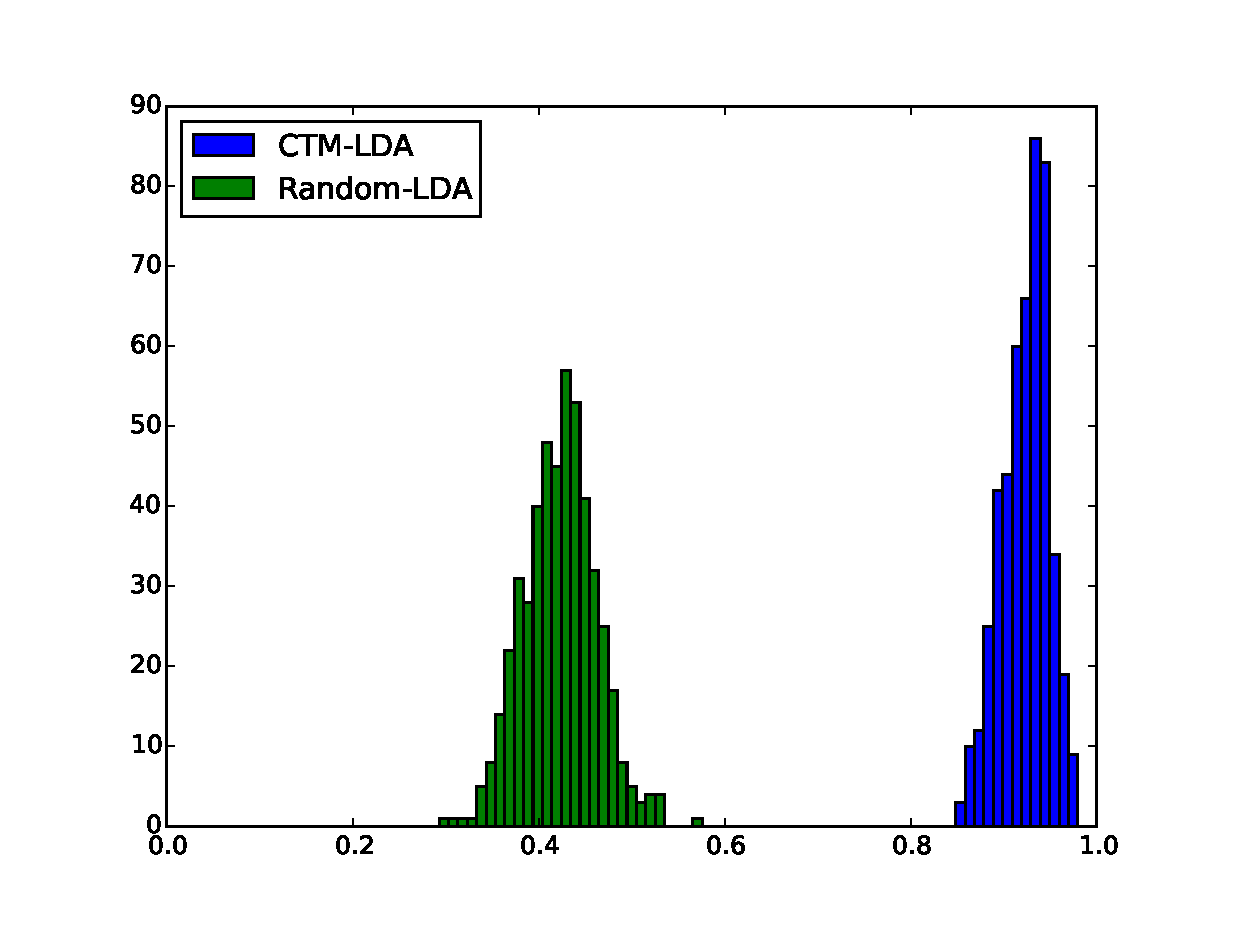
\includegraphics[width=\textwidth]{ctd-ctm-lda-diffs.eps}
\caption{Histograms of cosine similarities between the document-topic distributions $\theta$ inferred by LDA, CTM and CTM with exponentiation, with differences to random guessing plotted as a baseline}
\label{fig:ctd-ctm-lda-diffs}
\end{figure}

\subsection{CTD}

TODO: What is CTD?

The CTD dataset is a catalogue of drugs that lists which pathway each one of those affects. Not all pathways and not all drugs used in the KEGG/CMap dataset are mentioned in the CTD, so the final drug-pathway prediction matrices output by LDA and CTM had to be filtered down to the shape of CTD: 495 drugs (thus simply dropping the relevant rows) and 193 pathways (removing the columns and renormalising). The density of the resultant $\theta$ is 0.1231.

The theta values predicted by the models are then used to rank the pathways for every drug.

\begin{figure}[!htb]
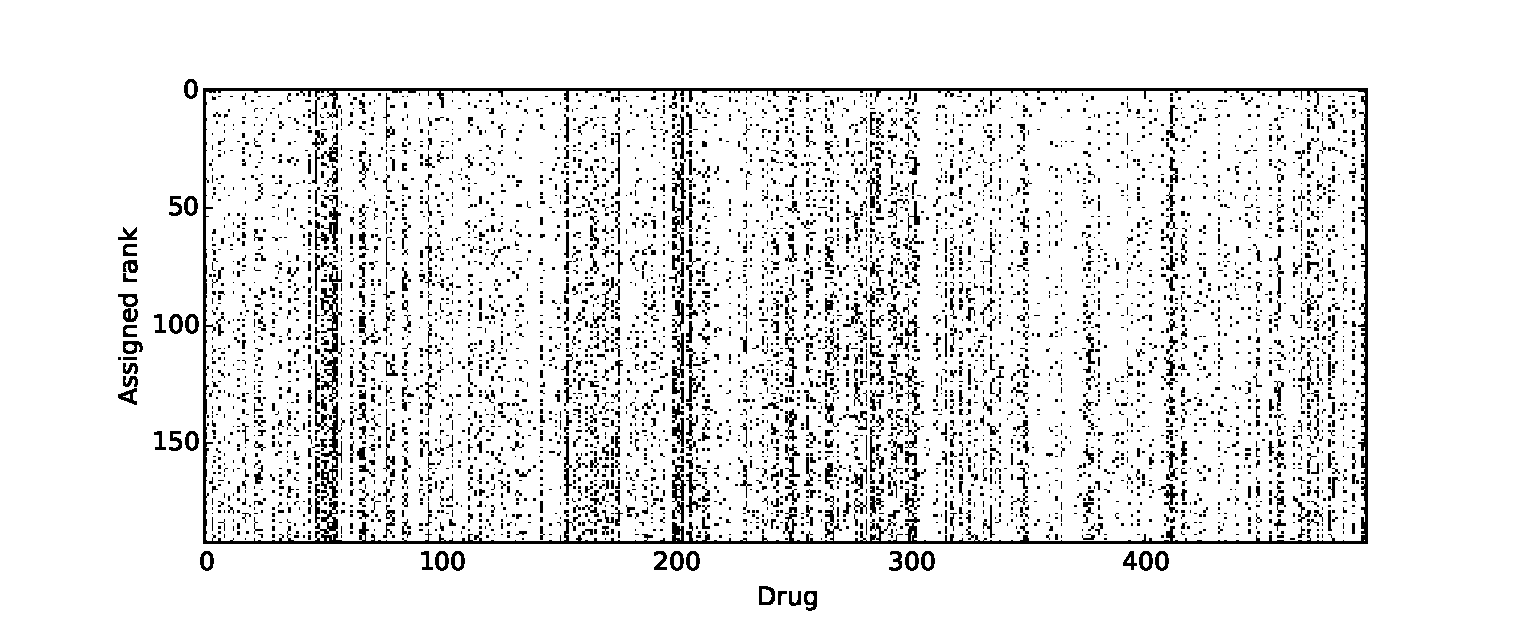
\includegraphics[width=\textwidth]{ctm-ctd-heatmap.eps}
\caption{CTD ``heatmap" for CTM}
\label{fig:ctm-ctd-heatmap}
\end{figure}

\begin{figure}[!htb]
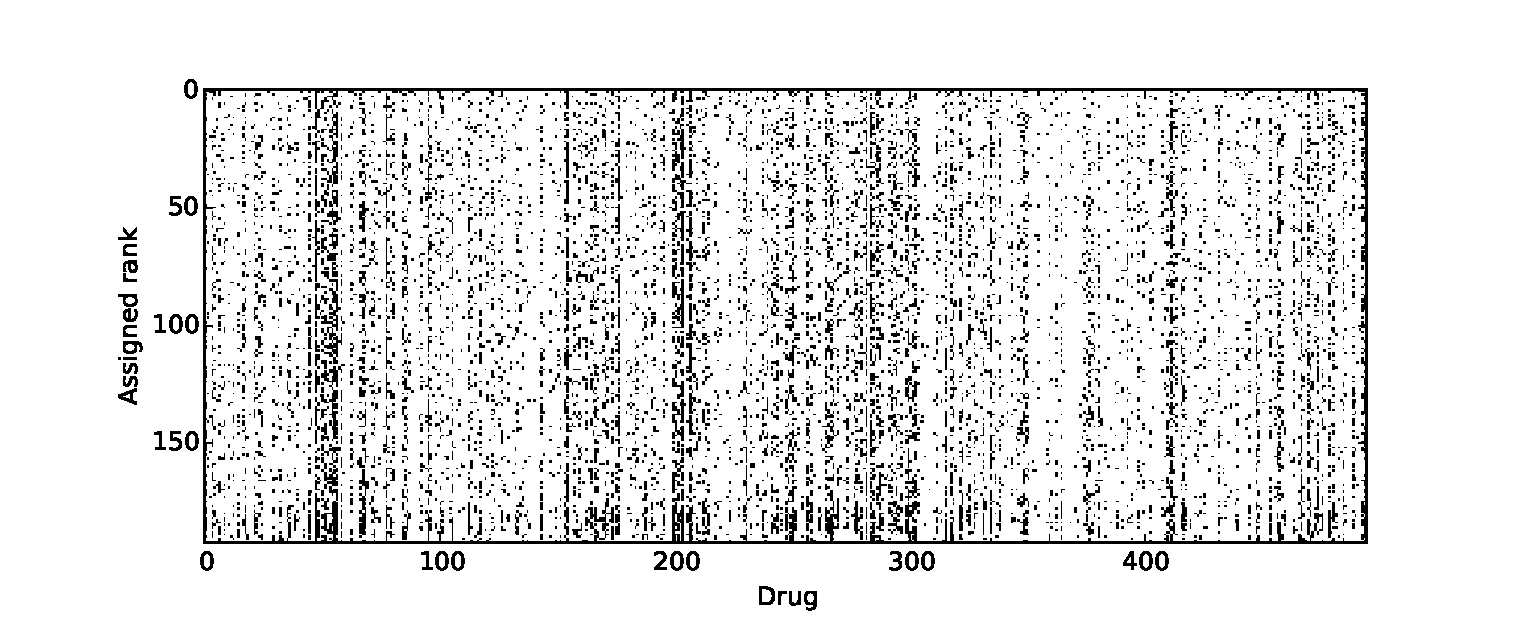
\includegraphics[width=\textwidth]{lda-ctd-heatmap.eps}
\caption{CTD ``heatmap" for LDA}
\label{fig:lda-ctd-heatmap}
\end{figure}

Figure~\ref{fig:ctm-ctd-heatmap} shows a so-called ``heatmap" for CTM, explained in the beginning of this section. The expected behaviour is for the black squares to cluster towards the top of the ``heatmap", since that means the model assigned the top ranks to pathways that are actually correct. However, both LDA (Figure~\ref{fig:lda-ctd-heatmap}) and CTM are very far from that and to see exactly how, a different visualisation is required.


\subsubsection{Precision-recall curves}

The precision-recall curves for the whole dataset are plotted in Figure~\ref{fig:ctd-pr-curves}.

\begin{figure}[!htb]
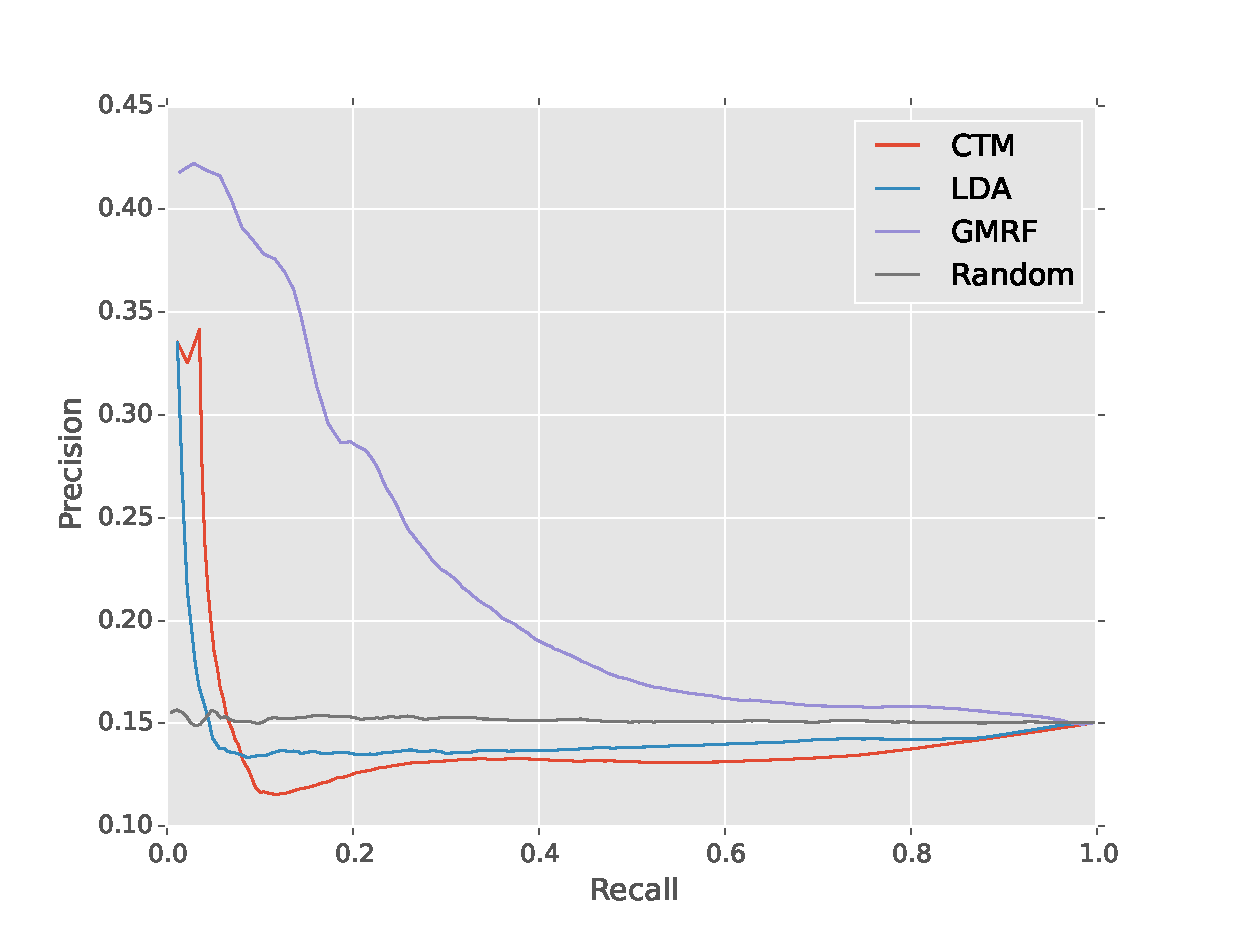
\includegraphics[width=\textwidth]{ctd-pr-curves.eps}
\caption{Precision-recall curves on the validation dataset (CTD) for CTM, LDA, and random topic assignments (baseline)}
\label{fig:ctd-pr-curves}
\end{figure}

TODO: what are MAP values?

TODO: move MAP values to a table

The MAP values for CTM, LDA and CTM with exponentiation are 0.181, 0.189 and 0.204, respectively. The average MAP value for random guessing is 0.172.

The main conclusion to be made from this is that while CTM does have some predictive power, since its performance is significantly different from the baseline, it, in fact, does not outperform LDA on this dataset. Exponentiating the gene expression data prior to training (and thus not discarding the sign), however, improves the performance of CTM beyond that of LDA.

One curious phenomenon on this graph is the large spike in precision at low recall levels, meaning that all models made multiple correct predictions at top ranks. Figure~\ref{fig:ctd-side-plot-10} shows this in more detail: it plots, in essence, the number of black squares in each model's ``heatmap" at every rank up to 10. For almost half of all the drugs, the three models' most expressed pathway is indeed confirmed by CTD to be affected by those drugs.

\begin{figure}[!htb]
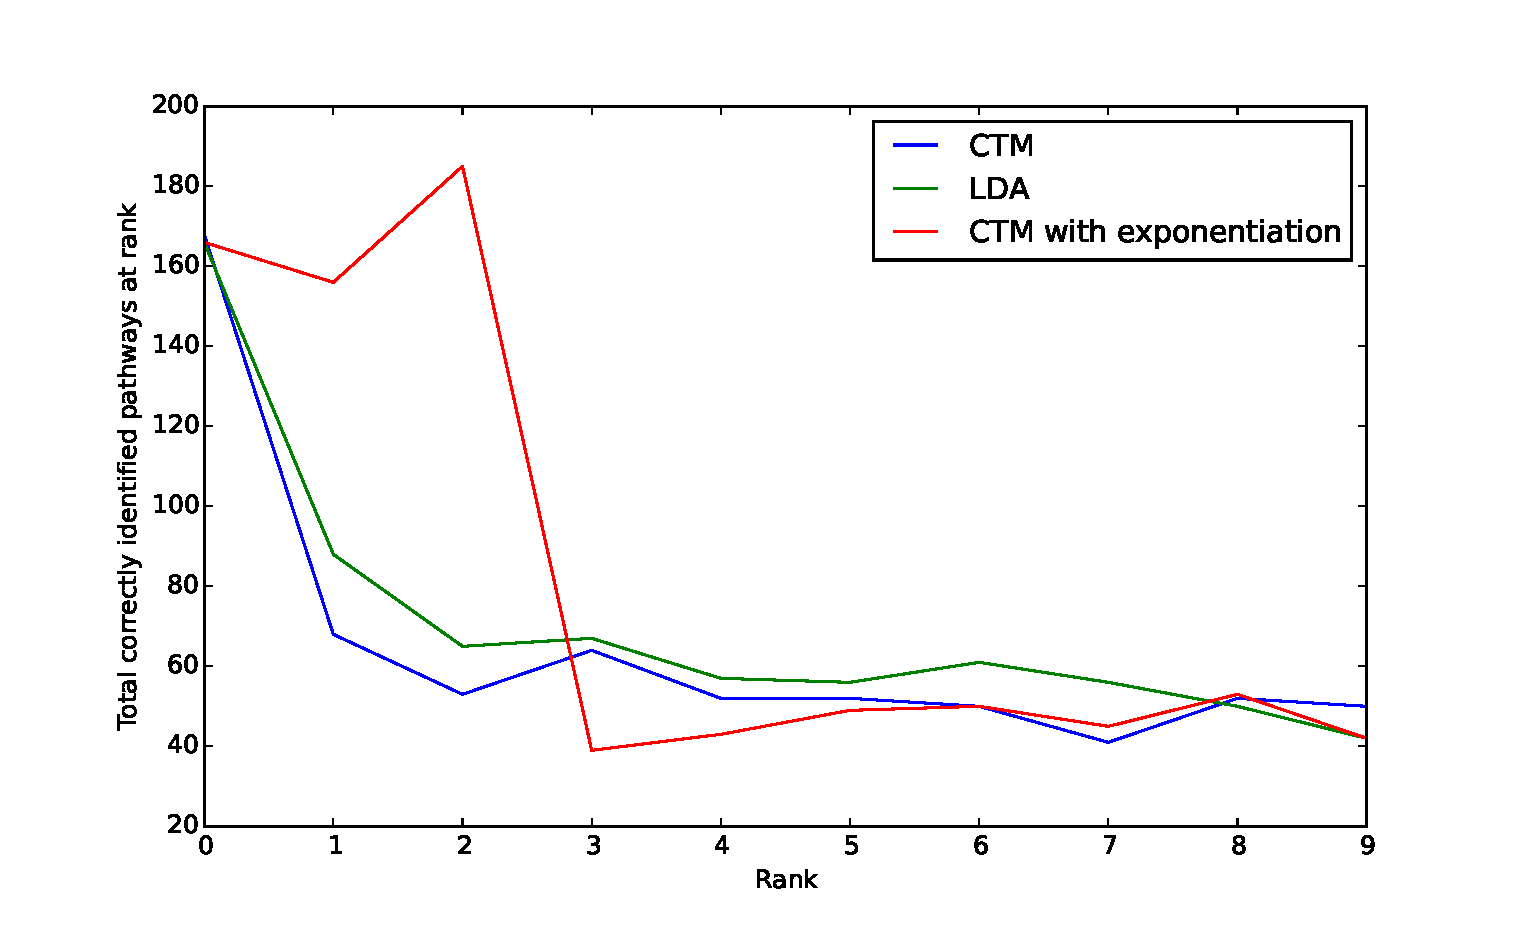
\includegraphics[width=\textwidth]{ctd-side-plot-10.eps}
\caption{Number of drugs with correctly identified pathways at each rank.}
\label{fig:ctd-side-plot-10}
\end{figure}

Closer inspection, however, reveals that the three models rank a pathway named ``Metabolic pathways" as first for most drugs in the evaluation set (495 (all drugs) for LDA, 480 for CTM and 474 for CTM with exponentiation). This pathway is a ``catch-all" for all metabolic pathways, uniting all pathways in the dataset. Ignoring it in the evaluation process changes the results tremendously.

\begin{figure}[!htb]
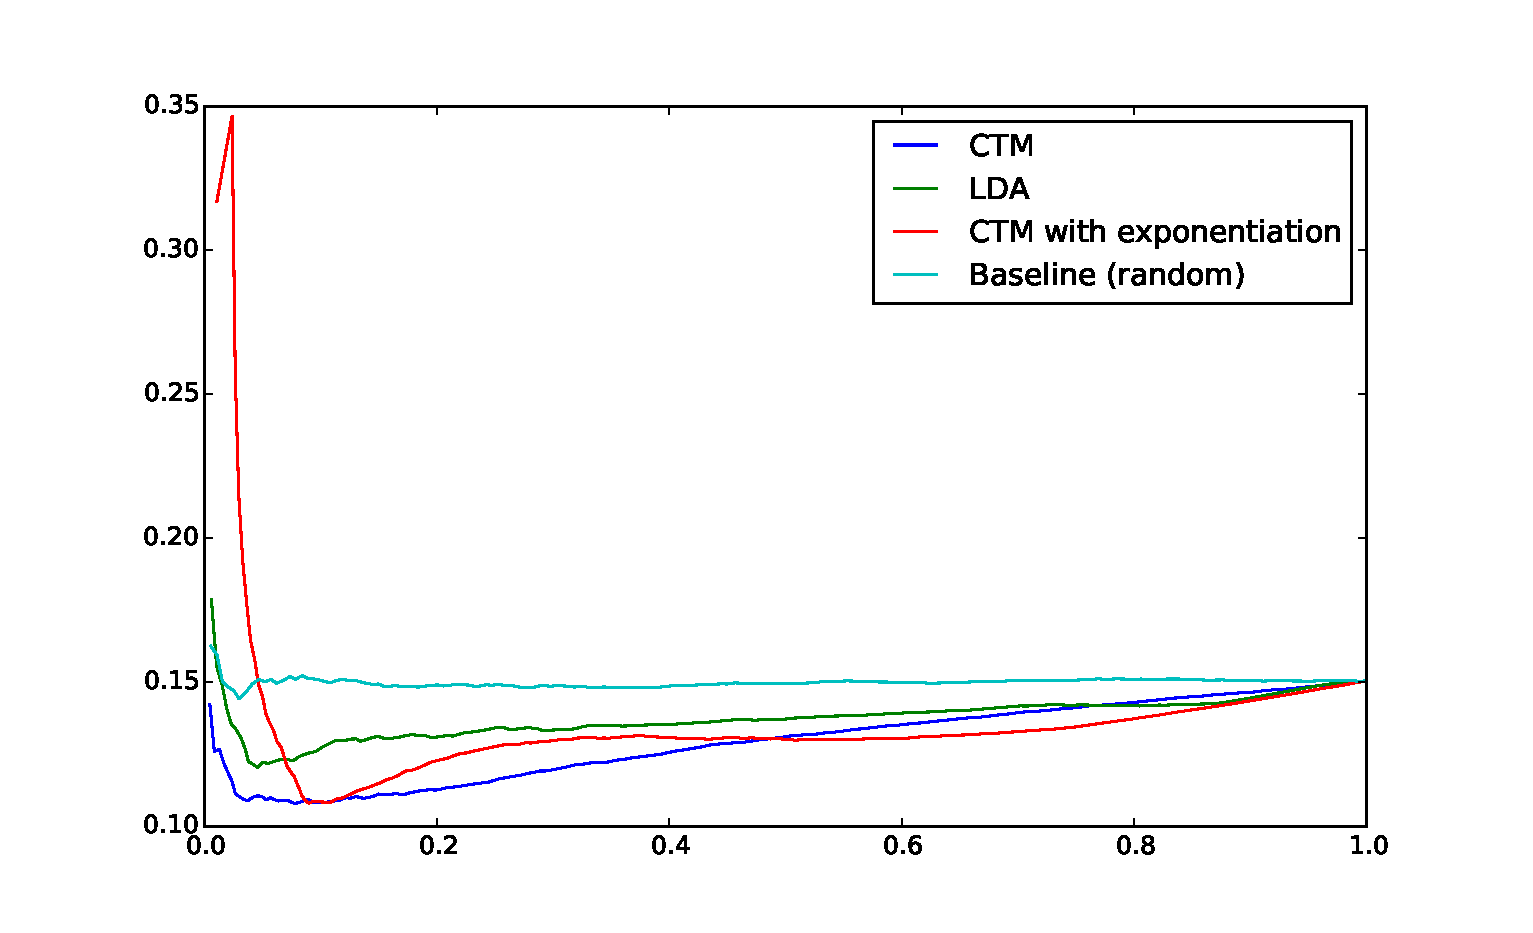
\includegraphics[width=\textwidth]{ctd-pr-curves-no1100.eps}
\caption{Precision-recall curves on the validation dataset with the ``Metabolic pathways" pathway excluded.}
\label{fig:ctd-pr-curves-no1100}
\end{figure}

Figure~\ref{fig:ctd-pr-curves-no1100} shows the resultant precision-recall curve. After exclusion, the MAP values for CTM, LDA and CTM with exponentiation are 0.166, 0.176 and 0.213, respectively, whereas the random method achieves a MAP value of 0.172. LDA still beats CTM and the fact that CTM relied on the presence of the removed pathway for most of its performance now has dropped its MAP value below that of random guessing. However, CTM with exponentiation now vastly outperforms all the other models.

TODO: the CTM ``side plot" seems to tend upwards with rank, so its predictions seem to be inverted. This is also confirmed by the Spearman rho: CTM's mean-median correlation is -0.06 (GMRF gets 0.06, LDA -0.02)

\subsubsection{Rho-normalised log scores}
Figure~\ref{fig:ctd-rho-cdf} shows the CDF plots (fraction of scores below a given value) of the rho-normalised log scores (Equation~\ref{eq:rho-normalised-score}) for CTM, LDA and CTM with exponentiation (with the ``Metabolic pathways" pathway excluded). It can be seen from the plot that the median score of all three models is below that of random guessing. The parameters of this distribution are summarised in table~\ref{tab:ctm-ctf-summary}. The performance of random in this case was obtained by simulating 1000 random drug-pathway distributions and averaging their mean performance.

\begin{figure}[!htb]
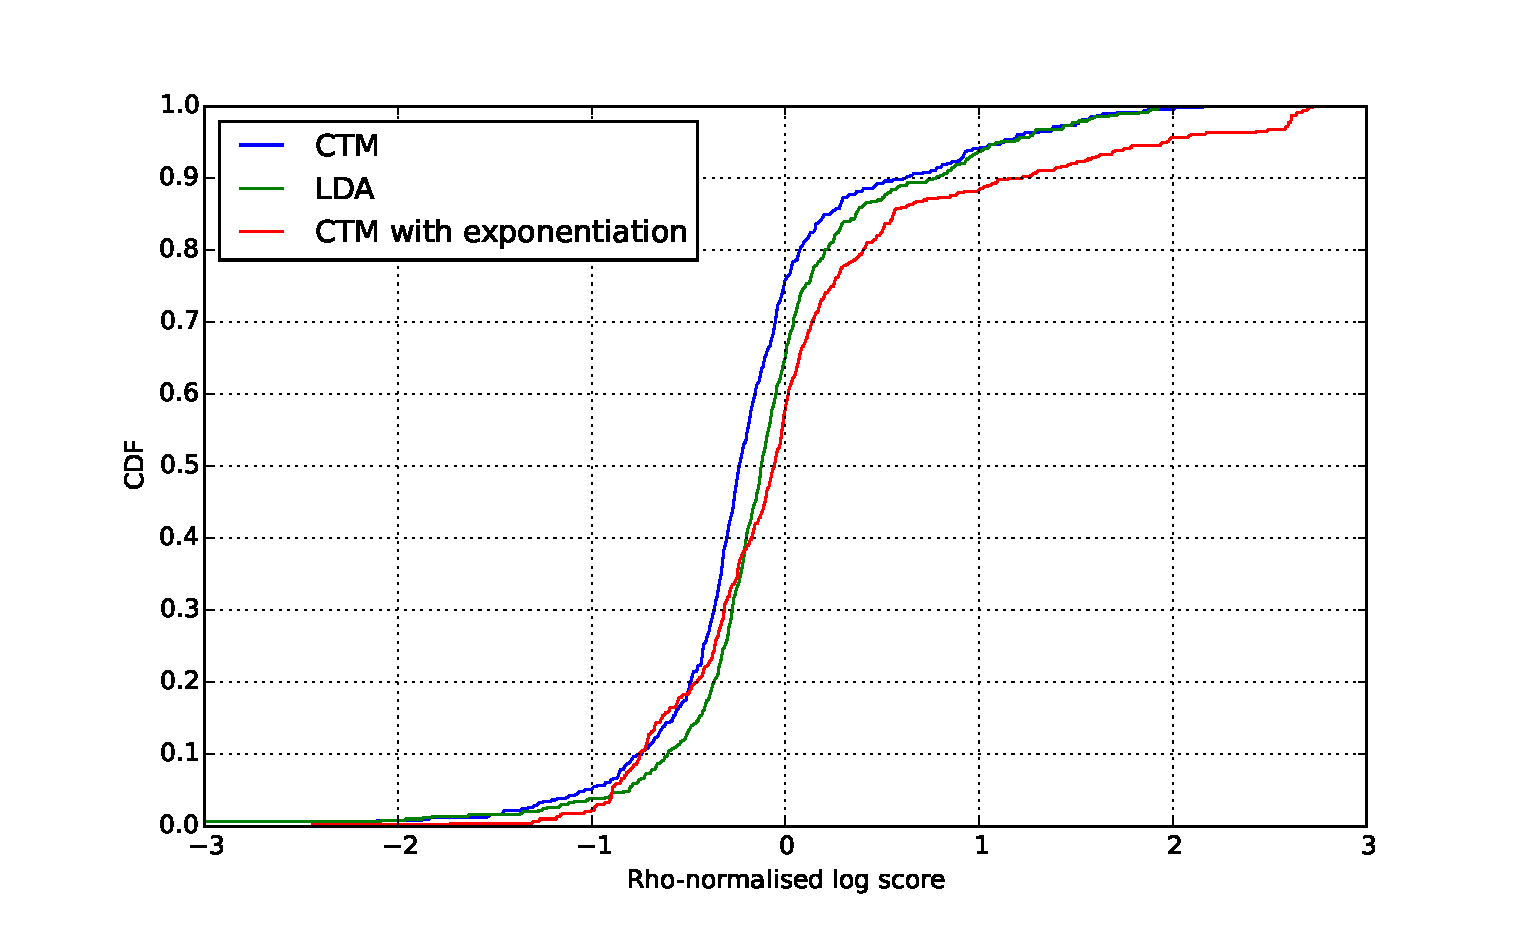
\includegraphics[width=\textwidth]{ctd-rho-cdf.eps}
\caption{Cumulative distribution function (CDF) of the rho-normalised log score of the models on the CTD data}
\label{fig:ctd-rho-cdf}
\end{figure}

\begin{table}
\begin{tabular}{| l | l | l | l |}
\hline
Model & Mean & Median & Standard deviation\\
\hline
CTM & -0.177 & -0.238 & 0.654 \\
LDA & -0.070 & -0.125 & 0.645 \\
CTM with exponentiation & 0.064 & -0.059 & 0.801 \\
Random & -0.008 & 0.000 & 0.124 \\
\hline
\end{tabular}
\caption{Parameters of the distribution of the rho-normalised log scores}
\label{tab:ctm-ctf-summary}
\end{table}

CTM with exponentiation is the only method that achieved a positive mean score, since its performance distribution has a heavy right tail: about 10\% of its predictions achieved a score greater than 1.

\subsubsection{1-iteration CTM}

\begin{figure}[!htb]
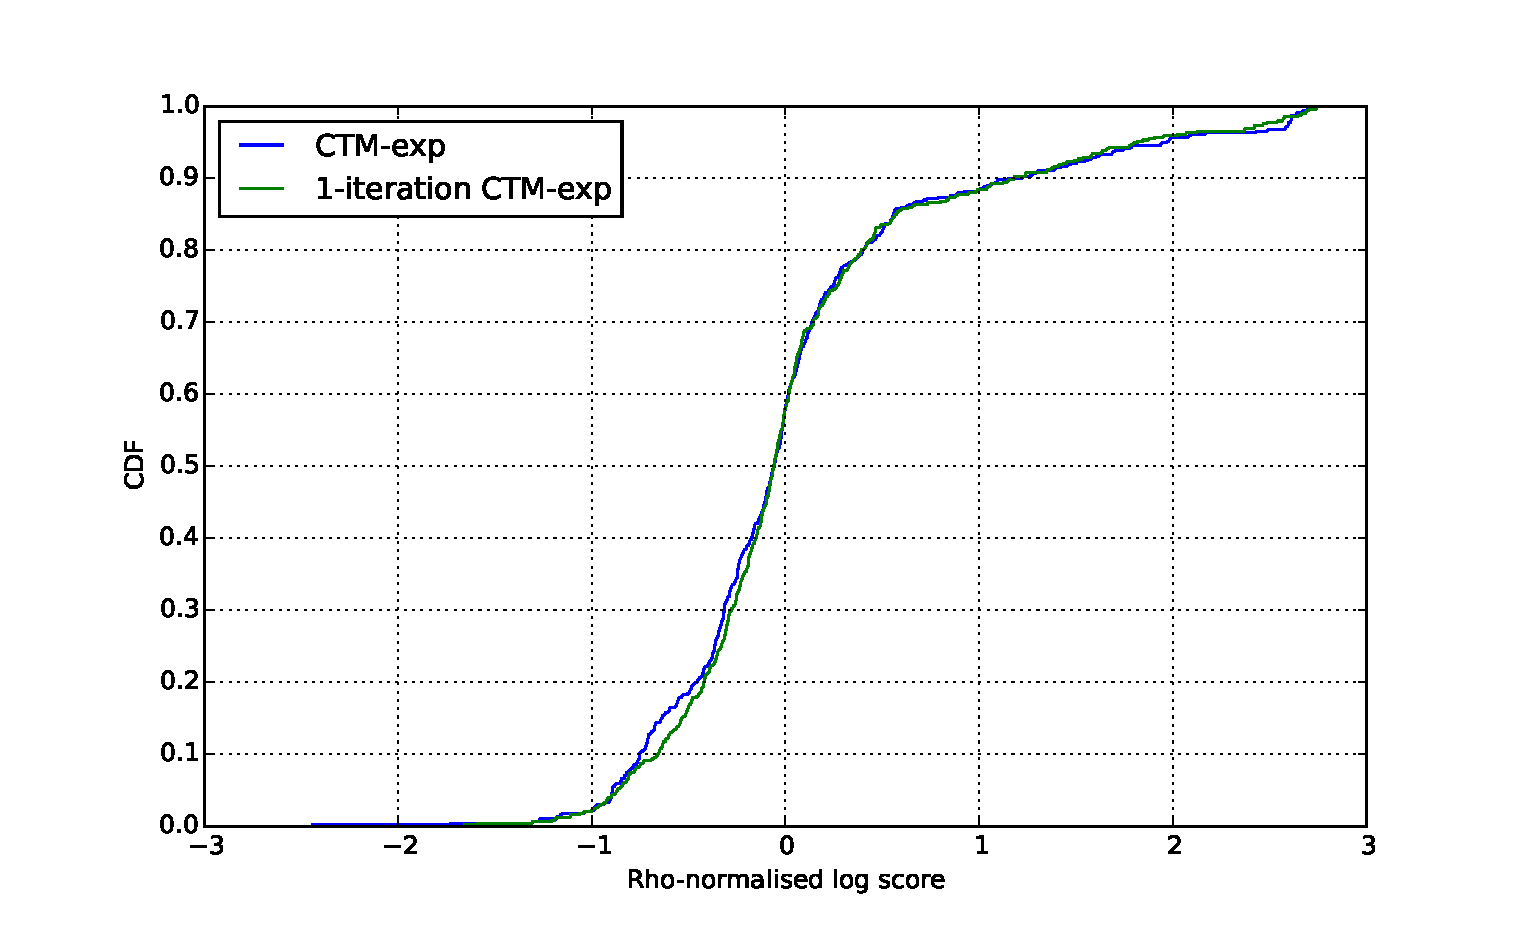
\includegraphics[width=\textwidth]{ctd-ctm-1iter-rho.eps}
\caption{CDF of the rho-normalised log scores for 1-iteration CTM with exponentiation, with full-convergence CTM plotted as reference}
\label{fig:ctd-ctm-1iter-rho}
\end{figure}

\begin{figure}[!htb]
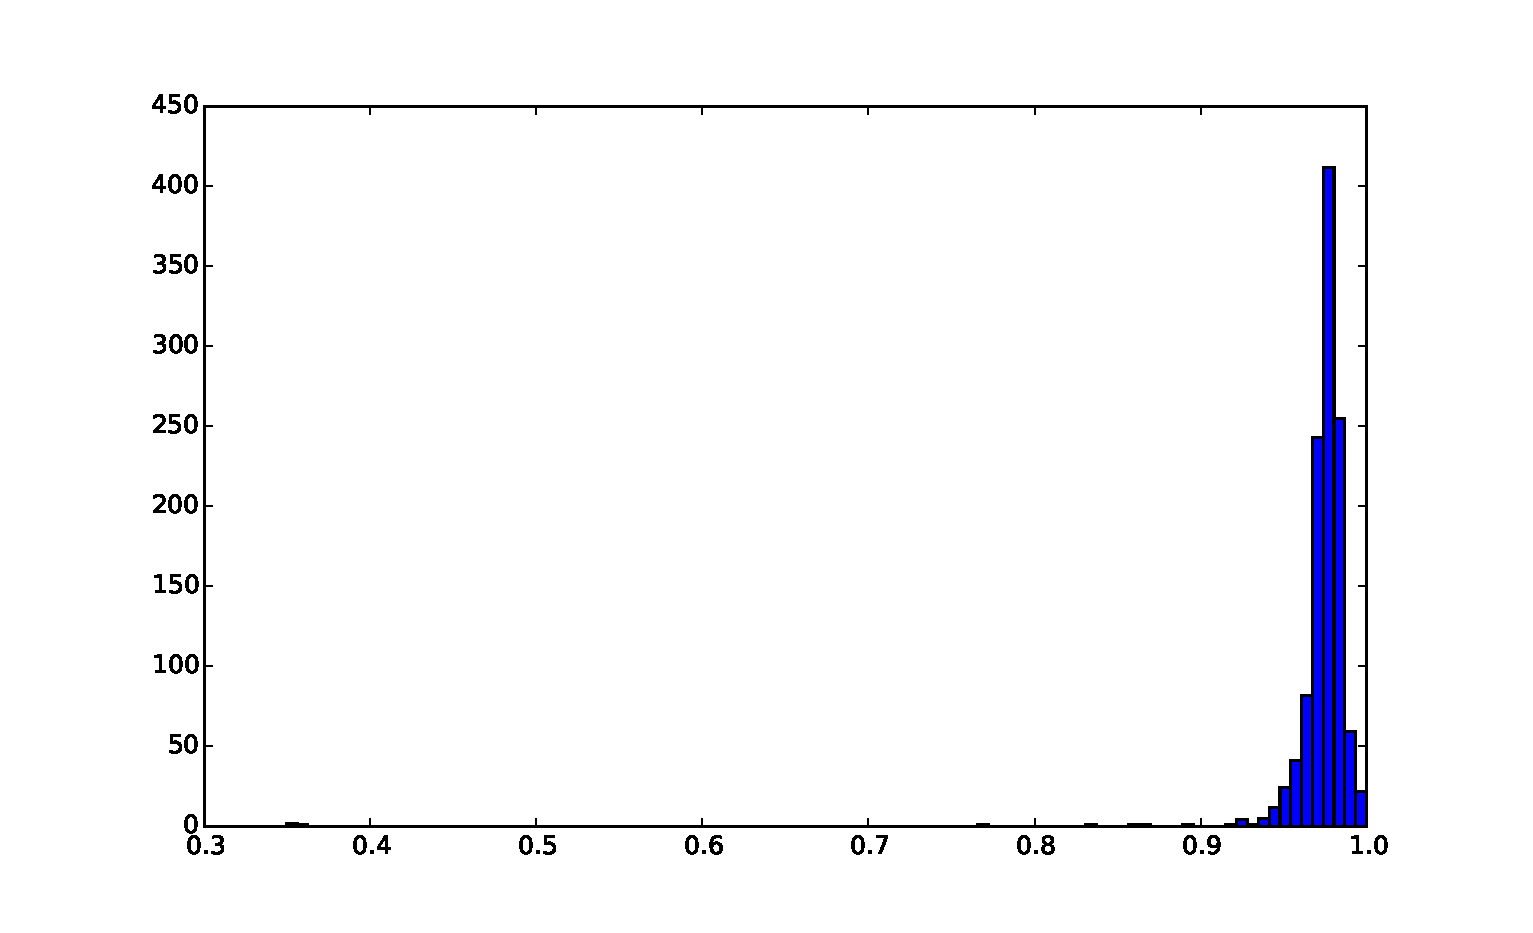
\includegraphics[width=\textwidth]{ctd-ctm-1iter-hist.eps}
\caption{Distribution of cosine similarities between drug-pathway distributions predicted by 1-iteration and full-convergence CTM-exp}
\label{fig:ctd-ctm-1iter-hist}
\end{figure}

Even after only 1 iteration of training, the predictions made by CTM with exponentiation are close to the prediction of CTM-exp after full convergence (Figure~\ref{fig:ctd-ctm-1iter-hist}). Figure~\ref{fig:ctd-ctm-1iter-rho} shows the cumulative plot of the rho-normalised log scores of 1-iteration CTM-exp to illustrate that its performance is also very close to the full-convergence CTM-exp at a fraction of training time. In fact, the mean score of CTM-exp is 0.080 (against full-convergence CTM-exp's 0.064) and it outperforms the previous CTM-exp on 256/492 (52\%) of all drugs in CTD.

\subsubsection{Performance as a function of drug density}

Since CTM takes into account the correlations between pathways, it could be the case that it will perform better with dense drugs (that affect multiple pathways) than LDA and will lose out to LDA on more sparse drugs. Figure~\ref{fig:ctd-ctm-lda-scatter} plots this relationship and there are some interesting observations to be made. The variance of the performance decreases with density, which could be because the final score is normalised by the drug density, so for small densities the variance of the performance is amplified. However, at low densities, the distribution of scores is asymmetric and the normalisation does not explain that. This asymmetry, in fact, causes the correlation between the score and the drug density to be negative.

\begin{figure}[!htb]
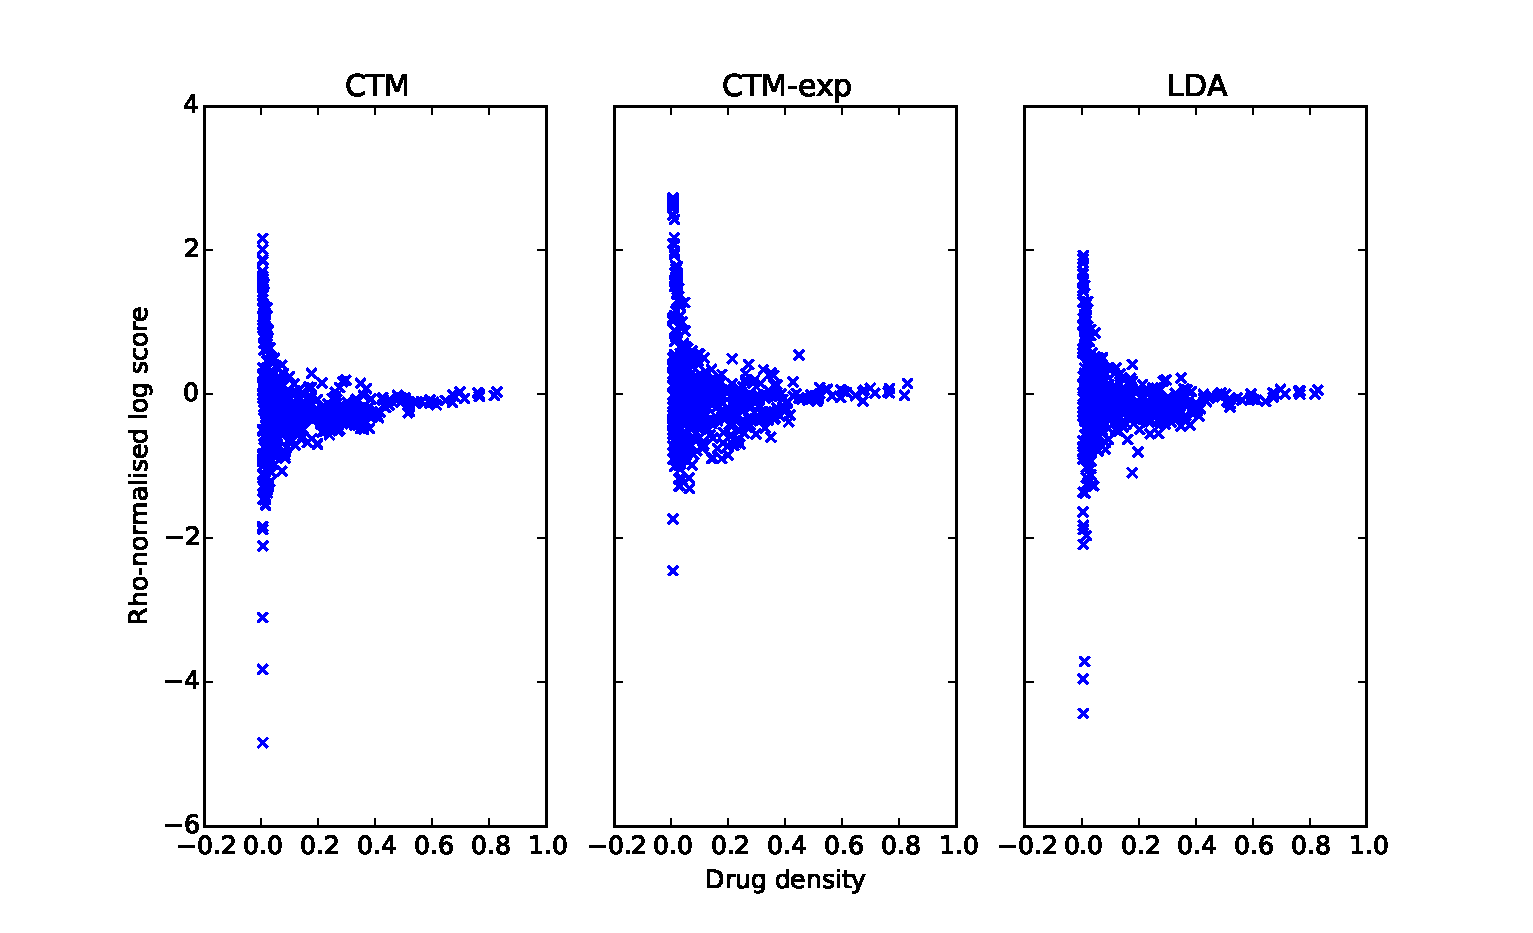
\includegraphics[width=\textwidth]{ctd-ctm-lda-scatter.eps}
\caption{Scatterplot of the rho-normalised log score versus the drug density for the three models}
\label{fig:ctd-ctm-lda-scatter}
\end{figure}

\begin{table}
\begin{tabu}{| l | l | l |}
\hline
Model & Pearson's r & Two-sided p-value \\
\hline
CTM & -0.042 & 0.353 \\
LDA & -0.074 & 0.102 \\
CTM with exponentiation & -0.186 & $3.60 \times 10^{-5}$ \\
\hline
\end{tabu}
\caption{Pearson's correlation coefficients between the drug density and the rho-normalised log scores}
\label{tab:ctm-density-correlation}
\end{table}

Table~\ref{tab:ctm-density-correlation} shows the Pearson's r score and the 2-tailed p-value, calculated by \texttt{SciPy}'s function \texttt{scipy.stats.pearsonr}. The p-value is defined as ``the probability of an uncorrelated system producing datasets that have a Pearson correlation at least as extreme as the one computed from these datasets" and so using this value, we can establish that there is a significant negative correlation between the performance of CTM with exponentiation and the drug density. This is because CTM-exp seems to have improved the worst outliers of CTM at low density levels.

\begin{table}
\begin{tabu}{| l | l | l |}
\hline
Criterion & Number of drugs & Mean density \\
\hline
CTM-exp outperforms LDA & 284 (57.7\%) & 0.148 \\
LDA outperforms CTM-exp & 208 (42.3\%) & 0.154 \\
\hline
\end{tabu}
\caption{Characterisation of drugs on which the models outperform each other}
\label{tab:ctm-lda-outperform}
\end{table}

Table~\ref{tab:ctm-lda-outperform} further shows that CTM does not win on higher-density drugs: the average density of drugs on which CTM with exponentiation achieves a higher score than LDA is slightly smaller than of those where LDA beats CTM.

\subsubsection{Clustering the drug similarity matrix}
Since the document (or drug) similarity matrix (\ref{eq:document_similarity_matrix}) is not affected by the topic identifiability, I decided to perform clustering on the matrix to identify some common groups of drugs and reference them to the actual descriptions of those drugs.
I used the Markov Clustering Algorithm (MCL)  \cite{Dongen:2000:CAG:868986}, a simple method that's based on the insight that a document similarity matrix, when normalised, forms a Markov chain. If one simulates multiple ``random walkers" on this chain and slowly starts weakening the links between the elements of the chain, each of them will eventually end up roaming around the final clusters. This is encoded in the following algorithm:

\documentclass{article}
\usepackage[noend]{algpseudocode}
\usepackage[]{algorithm}
\usepackage{amsmath}
\usepackage[cm]{fullpage}
\newcommand{\var}[1]{{\operatorname{\mathit{#1}}}}

\begin{document}
\begin{algorithm}
	\caption{Markov Clustering Algorithm}
	\label{markov-clustering}
	\begin{algorithmic}[0]
		\Function{markov-clustering}{$M, \var{expansion}, \var{inflation}$}
			\While{change in $M >$ threshold}
				\State Normalize $M$
				\State Expansion step: $M \gets M^{\var{expansion}}$
				\State Inflation step: $M_{i,j} \gets M_{i,j}^{\var{inflation}}$
			\EndWhile
			\State Normalize $M$
			\State\Return $M$
		\EndFunction
	\end{algorithmic}
\end{algorithm}

\end{document}

The algorithm consists of repeatedly performing expansion and inflation on the transition matrix: in the expansion step, we exponentiate every element of the matrix (thus weakening the links between different elements) and in the inflation step, we exponentiate the matrix itself (thus turning it into an $\mathit{inflation}$-step transition matrix and simulating the ``random walkers").

This process is guaranteed to converge on most graphs and the result can be interpreted as follows: if $M_{i,j} > 0$, then $j$ is a member of the cluster whose main ``attractor" is $i$. This value will usually be 1, meaning each element can only be a member of one cluster, but in case of some symmetric graphs it can be a fraction.

TODO: about expansion/inflation parameters

TODO: pictures + clustering for sigma as well

\subsection{ATC classification}

The World Health Organisation maintains a classification system for drugs called the Anatomical Therapeutic Chemical (ATC) Classification System. It's an hierarchical code that depends on the system in the body on which the drug acts. For example, caffeine has the code N06BC01, composed of:

\begin{itemize}[noitemsep]
\item Anatomical main group: \textbf{N} for Nervous system
\item Therapeutic main group: \textbf{06} for Psychoanaleptics
\item Therapeutic/pharmacological subgroup: \textbf{B} for Psychostimulants
\item Chemical/therapeutic/pharmacological subgroup: \textbf{C} for Xanthine derivatives
\item Actual substance: \textbf{01} for caffeine
\end{itemize}

There are a total of 13 anatomical main groups, defining the type of the system the drug is acting on. It is possible to train a powerful generic classifier such as Random Forest\cite{Breiman:2001:RF:570181.570182} that had successes in predicting drug-pathway perturbations\cite{Riddick15012011} on feature vectors $\theta_d$ inferred by LDA and CTM and anatomical main groups (as labels). This is another way to see whether the outputs of the topic models have any predictive power on the real-world data.

A Python package callied \texttt{scikit-learn} \cite{scikit-learn} that's deeply integrated with the \texttt{NumPy}/\texttt{SciPy} stack offers multiple classifiers and evaluation tools. Since implementing a Random Forest classifier was not an aim of this project, I gladly used those (Figure~\ref{fig:atc-python}). I hence performed 10-fold cross-validation on the classifier: split the $\theta_d$--label pairs into 10 sets, train the model on 9 of those and calculate the score reported by the model on the final set (for the Random Forest classifier, it's the fraction of correctly assigned classes). This is repeated another 9 times, each time with a different subset being held out from training. This allows to evaluate the model on more data than a single cross-validation cycle and also enhances the precision of the estimate.

\begin{figure}
\begin{Verbatim}[fontsize=\scriptsize]
def atc(thetas):
    from sklearn.ensemble import RandomForestClassifier
    from sklearn import cross_validation

    atc = pd.read_csv(diss_data_root + "ATC_codes_and_drug_names.csv")

    #Remove drugs not in ATC
    drug_names_in_atc = set(atc['DrugName']).intersection(drug_names)
    filtered_thetas = np.array([t for t, dn in zip(thetas, drug_names) if dn in drug_names_in_atc])
        
    #Turn the letter labels into indices
    labels = list(atc[atc['DrugName'].isin(drug_names_in_atc)]['ATC code'])
    label_map = {l: i for i, l in enumerate(sorted(set(labels)))}
    labels = [label_map[l] for l in labels]
    
    #Create the classifier (100 trees, 8 threads) and cross-validate
    forest = RandomForestClassifier(n_estimators=100, n_jobs=8)
    samples = cross_validation.cross_val_score(forest, filtered_thetas, labels, cv=10)
    return (np.mean(samples), np.std(samples))
\end{Verbatim}
\caption{Python code that performs the evaluation of the drug-pathway distributions using Random Forest}
\label{fig:atc-python}
\end{figure}

\begin{table}
\begin{tabu}{| l | l | l |}
\hline
Features & Mean RF score & SD of the RF scores \\
\hline
$\theta$ of CTM & 0.259 & 0.032 \\
$\theta$ of CTM-exp & 0.141 & 0.035 \\
$\theta$ of LDA &  0.201 & 0.035 \\
Random $\theta$ & 0.148 & 0.034 \\
Raw gene expression data (not exponentiated) &  0.748 & 0.133 \\
Raw gene expression data (exponentiated) &  0.746 & 0.131 \\
\hline
\end{tabu}
\caption{10-fold cross-validated mean accuracies for Random Forest on the ATC dataset for various feature sets}
\label{tab:atc-test-results}
\end{table}

Table~\ref{tab:atc-test-results} shows the mean scores and their standard deviation for different vectors used as features. The results here are almost the reverse of ranked evaluation on the CTD dataset. First of all, CTM with exponentiation did not perform significantly better than training the classifier on randomly drawn vectors. In fact, from an information-theoretic perspective, if there is no information in the feature vectors, the best score classifier can get is $2^{-H}$ where $H$ is the entropy of the distribution of labels: $2.41$ bits in the case of the ATC anatomical main groups, giving the average probability of guessing the right label of about $0.188$.

Secondly, LDA outperforms CTM-exp, and interestingly, CTM outperforms all other topic models in this case. However, all of these models are dwarfed by the performance of using the raw gene expression data (exponentiated or unexponentiated) to predict the anatomical main group of a drug.

\chapter{Conclusion}

%%%%%%%%%%%%%%%%%%%%%%%%%%%%%%%%%%%%%%%%%%%%%%%%%%%%%%%%%%%%%%%%%%%%%
% the bibliography
\addcontentsline{toc}{chapter}{Bibliography}
\bibliography{bibliography}

%%%%%%%%%%%%%%%%%%%%%%%%%%%%%%%%%%%%%%%%%%%%%%%%%%%%%%%%%%%%%%%%%%%%%
% the appendices
\appendix

\chapter{Project Proposal}

\documentclass[12pt,a4]{article}
\usepackage{hyperref}
\usepackage{color}
\usepackage{fullpage}
\begin{document}

\vfil


\begin{flushright}
\large{A. I\v{s}kovs}\\
\texttt{ai280}\\
Trinity College
\end{flushright}

\vspace*{\fill}
\begin{center}{\large Computer Science Tripos, Part II Project Proposal}

\vspace{0.3in}
\textbf{\center{\Large Predicting drug-pathway interactions using the Correlated Topic Model}}

\vspace{0.4in}
\centerline{\large \today}
\end{center}
\vspace*{\fill}

\vfil

%
%\noindent{\bf Project Originator:} N. Pratanwanich
%\vspace{0.4in}
%
%\noindent
%{\bf Project Supervisor:} N. Pratanwanich\\
%
%\noindent
%{\bf Signature:}
%\vspace{0.2in}
%
%\noindent
%{\bf Director of Studies:} Dr A. C. Norman\\
%
%\noindent
%{\bf Signature:}
%\vspace{0.2in}
% 
%\noindent
%{\bf Project Overseers:} Dr~A.~V.~S.~Madhavapeddy  \& Dr~S.~H.~Teuffel\\
%
%\noindent
%{\bf Signatures:}

\pagebreak

% Main document

\section*{Introduction}

Latent Dirichlet Allocation\cite{Blei} is a bag-of-words topic modelling algorithm that treats documents in a corpus as being generated by picking a set of topics and then drawing words from those topics. Using a sampling method, the posterior distributions of unknown variables (probability distributions of topics and words within topics) are inferred. This allows, for an arbitrary document, to infer a probability distribution of topics which it is about.

The 2014 paper\cite{Pratanwanich2014} by Naruemon Pratanwanich and Pietro Lio describes a model based on this algorithm to predict drug-pathway relationships: differential gene expression profiles of drug treatments are treated as documents, pathways where genes are functionally grouped as topics and genes as words. The model had to be augmented with priors: the pathway-gene relationships for some pathways are already known. In the end, this method provided better predictive results of pathways activated by certain drugs than the state-of-the art methods.

A problem with Latent Dirichlet Allocation and hence this approach is that it assumes that the topics (or pathways) are uncorrelated. This assumption is usually not true: a document about Computer Science is more likely to be about Mathematics than, say, Geology. Another 2014 paper\cite{C4MB00014E} by Naruemon Pratanwanich and Pietro Lio presents a model that assumes pathway crosstalk (correlation). It uses matrix factorisation together with this assumption to predict pathway responsiveness for drugs that affect multiple pathways and finds that using the correlation assumption results in a better fit to the gene expression data.

The Correlated Topic Model\cite{2007} was proposed as an improvement on the Latent Dirichlet Allocation: instead of using the Dirichlet distribution to model the relative proportions of topics in a document, it uses the logistic normal distribution. The parameters of the distribution are the mean and the covariance matrix, which allows for modelling correlations between topics. The original paper\cite{2007} uses a deterministic approach called Variational EM (Expectation Maximization) to train this model (due to the non-conjugacy of the logistic normal, the Markov Chain Monte Carlo approach with Gibbs Sampling is intractable). The Correlated Topic Model fit the sample corpus (a set of articles from \textit{Science}) better than LDA\cite{2007}.

Since the matrix factorization model that assumed pathway correlation\cite{C4MB00014E} and the LDA method\cite{Pratanwanich2014} outperform matrix factorization without correlations, it is suspected that adapting the CTM to the problem of prediction of pathway responsiveness to drug treatment would yield another improvement in predictive power.

The aim of this project is to implement and test such a model. In addition to reusing the Bayesian network from the CTM, the model will be augmented with a prior distribution of known gene-pathway relationships. The equations for training the model will be derived, based on the existing CTM equations for Variational EM\cite{2007}. The model will be tested on a synthetic corpus of drug gene expression data for model verification and then on publically available datasets (CMAP\cite{CMap} for gene expression data and KEGG\cite{KEGG} for pathway data). The results will be compared with the latent variables inferred by the LDA approach. While it's not possible to guarantee that the model will perform better in every case, the results will be investigated to see in which cases the LDA approach performs better than CTM and vice versa.

\section*{Starting Point}

I know Python and have some experience in working with the SciPy stack. Python has lots of facilities for data processing and while it is an interpreted language, NumPy uses native LAPACK/BLAS (linear algebra) libraries as a backend. This means that the performance of the linear algebra routines is on par with C.

Since this project uses some concepts from the Artificial Intelligence II course (see Key Concepts), I will have to familiarise myself with the course before it begins.

There exists an R package for the Correlated Topic Model, as well as a C implementation of the Model written by the authors of the original paper (\url{https://www.cs.princeton.edu/~blei/ctm-c/}). I will however only be able to use those as a reference at most: adding priors to the model will change its implementation. On the other hand, the C implementation has a way to perform posterior inference (prediction) on new documents, which can help with one of the extensions to the project.

\section*{Substance and Structure of the Project}

\subsection*{Key Concepts}

The key concepts in this project are drawn from the Artificial Intelligence II course, including topics such as Bayesian Networks and inference, methods for training and evaluating classifiers and probability distribution transformation. This project, however, will go beyond the scope of the course, touching on Variational Inference, conjugate and non-conjugate distributions and Expectation Maximization.

\subsection*{Major Work Items}

\subsubsection*{Required Reading and Research}

\begin{itemize}
\item Artificial Intelligence II Lecture notes: introduction to Bayesian networks and inference
\item Chapters 9 and 10 of Christopher Bishop's book\cite{Bishop:2006:PRM:1162264} on computer vision models: Mixture models (of which LDA and CTM are variations) and the Expectation Maximization algorithm, as well as Variational Inference.
\item ``Build, Compute, Critique, Repeat: Data Analysis with Latent Variable Models"\cite{doi:10.1146/annurev-statistics-022513-115657}, an introduction to latent variable models that describes how to train the models using mean-field Variational Inference, use them to perform predictions and evaluate them.
\item The original LDA\cite{Blei} and CTM\cite{2007} papers to understand the structures of the respective generative probabilistic models and their inference based on Variational EM.
\item Naruemon Pratanwanich and Pietro Lio's paper\cite{Pratanwanich2014}  on adapting LDA in order to familiarize myself with how microarray data is preprocessed into a pseudo-drug ``document", how the gene-pathway membership priors are incorporated into the model, as well as the ranking method used to evaluate its performance.

I will also need to get a better understanding of the biological context around the project, including topics such as genes, pathways, how the drug gene expression data is obtained using microarrays and how it has to be preprocessed.

\end{itemize}

\subsubsection*{Developing a Model}

The classic Expectation Maximization algorithm consists of two steps:

\begin{itemize}
\item \textbf{E}: Calculate the expected value of the log likelihood of seeing the latent variables given the observed variables and the model parameters.
\item \textbf{M}: Maximize this function by updating the model parameters.
\end{itemize}

The CTM paper\cite{2007} applies an algorithm called Variational EM that, using a variational distribution, approximates the posterior distributions of latent variables with respect to the model parameters in the \textbf{E} step and estimates the model parameters with respect to variational parameters in the \textbf{M} step.

I have to understand and alter this algorithm in order add prior information on gene-pathway memberships to the model.

\subsubsection*{Implementation and Testing}

In Python, implement:

\begin{itemize}
\item The software to generate synthetic data for model verification and to preprocess real datasets.
\item The actual Correlated Topic Model that incorporates the priors.
\end{itemize}

During development, the model will be tested using toy datasets of synthetic gene expression and pathway data. Using the real datasets, it will then be compared against the LDA method (see Evaluation and Success Criteria).

\subsubsection*{Fallback Plan}
In case I fail to incorporate priors into the Correlated Topic Model, I will use one of the available libraries for fitting the CTM and instead work on processing the gene data into a drug "document" that can be understood by the library, as well as developing a way to predict pathway distributions for a previously unseen drug. The evaluation procedure in that case will have to be changed, since not having priors in the model will mean that the pathways will be completely arbitrary and will not correspond to real drug data.

Another option is using a less complicated algorithm such as Random Forests that has high predictive power on drug-pathway perturbations\cite{Riddick15012011}. In that case the setting will be that of supervised learning, where the training data are known pairs of drugs and pathways and the features are the differential gene expression data. However, in this case I won't be able to test the hypothesis of pathway correlation and how the data are generated as I would be able to by using the aforementioned generative probabilistic models.

\section*{Evaluation and Success Criteria}

The \textbf{main criterion} for success is a working implementation of the model as per its specification. This will be evaluated as follows:
\begin{itemize} 
\item Generate a toy dataset of random pathways, pathway-gene memberships (a probability distribution over genes) and drug-pathway interactions (a probability distribution over pathways)
\item Use that to generate a corpus of gene expression data as per how the Correlated Topic Model assumes it's generated.
\item Together with a random subset of the pathway-gene membership data to serve as a prior, use the model to infer the latent variables and compare them with the ones that generated the dataset.
\end{itemize}

Note that the successful achievement of this objective does not imply the model has any predictive power for real drug data. It only verifies that the model works as expected and there are no errors in the implementation.

The comparison with the LDA method can be performed in two ways. Firstly, the model can be run on the CMAP/KEGG datasets to infer the latent variables. One of these is the per-drug pathway distribution, which can then be compared with the distribution inferred by the LDA method based on the accuracy on the reference data. It is possible that the developed model will perform better on some drugs than LDA and worse on others. This will be investigated in order to know which types of drugs it's better to use one model over another.

In case \textbf{the extension goal} of having a method for predicting pathways activated by certain drugs has been reached, the model will be tested on reference data (known drug-pathway relationships). This will be done by performing the predictions for known drugs and then using the pathway ranking metric described in\cite{Pratanwanich2014}.


\section*{Extensions}
The original CTM paper does not explicitly mention how the CTM can be used to calculate the topic proportions for a new document. One extension would hence involve performing that, in which case it will be possible to better compare the performance of the model with the LDA approach using the ranking method described in the paper\cite{Pratanwanich2014} (without this extension, we can still compare the results by considering the latent variables that both models inferred from the data).

Yet another extension can be making an interface for the trained model in order to create a stand-alone tool that researchers can use.

There are multiple other priors that can be incorporated into the model to improve predictive power, for example, the correlation between drugs: the molecular structure of a drug can be treated as a set of functional groups and so drugs with similar sets of functional groups are likely to have similar effects.

In addition, the Variational EM approach only gives a maximum likelihood estimate of the model parameters. The model could be given a full Bayesian treatment by using hierarchical Bayesian modelling on the model parameter. This may help solve the known problem of singularity of the covariance matrix when there is a large number of topics\cite{Masada:2013:RIC:2525761.2525819}.

\section*{Resource Declaration}

The data for pathways will be taken from the KEGG\cite{KEGG} database and the drug gene expression data will be taken from CMAP\cite{CMap}, which are publically available.

I will be using my own laptop for main development, a quad-core machine with Windows and ArchLinux on it. The source code will be kept in a Git repository which will be regularly pushed to GitHub, as well as to my MCS filespace. As the KEGG and CMAP data is publically available, and the code used to read and prepare it for processing will be backed up, I do not expect to require to make backups of the actual datasets.

\section*{Timetable: Workplan and Milestones to be achieved.}

Planned starting date is 27/10/2014.

\begin{enumerate}

\item {\bf 27/10/2014 -- 09/11/2014} 

Perform required reading and research (as per the Major Work Items section). Set up the outline for the dissertation.

\item {\bf 10/11/2014 -- 23/11/2014} 

Modify the model and adapt the equations used for inference to incorporate priors. Start writing the Method section of the dissertation.

\item {\bf 24/11/2014 -- 11/01/2015} 

Implement the model in Python. Generate a small toy dataset to verify the implementation. Debug the code.

\item {\bf 12/01/2015 -- 25/01/2015}

Work on optimizing and debugging the code so that it can run in reasonable time on a large toy dataset. Write the progress report. Continue writing the Method and start writing the Evaluation sections of the dissertation.

\textbf{Milestone:} a working implementation of the modified model. 

\item {\bf 26/01/2015 -- 08/02/2015} 

Submit the progress report. Rehearse and deliver a presentation to the overseeing group.

Obtain and explore the KEGG and the CMAP datasets. Preprocess the data into a suitable format for the model.

\item {\bf 09/02/2015 -- 22/02/2015}

Derive the equations required for prediction of pathways that are perturbed given a new drug (extension 1).

\item {\bf 23/02/2015 -- 08/03/2015}

Use the CMAP/KEGG datasets to train the model and evaluate it against the performance of the LDA model.

\item {\bf 09/03/2015 -- 19/04/2015}

Work on the remaining extensions to the project (such as packaging the model as a stand-alone tool) and continue writing the dissertation.

\item {\bf 20/04/2015 -- 03/05/2015}

Finish writing a draft dissertation. Submit to the Director of Studies and the Supervisor for review, allowing 2 weeks to read the draft.

\item {\bf 04/05/2015 -- 10/05/2015}

Incorporate comments from the reviews. Submit the dissertation.

\end{enumerate}

\bibliographystyle{unsrt}
\bibliography{bibliography}

\end{document}

\end{document}
